%\pdfoutput=1
% Uncomment line above if submitting to arXiv and using pdflatex

% $Id: main.tex 124030 2018-10-12 09:08:33Z pkoppenb $
% ============================================================================
% Purpose: Template for LHCb documents
% Authors: Tomasz Skwarnicki, Roger Forty, Ulrik Egede
% Created on: 2010-09-24
% ============================================================================
\documentclass[12pt,a4paper]{article}
%%\documentclass[12pt,letter]{article}
% For two column text, add "twocolumn" as an option to the document
% class. Also uncomment the two "onecolumn" and "twocolumn" lines
% around the title page below.

% Variables that controls behaviour
\usepackage{ifthen} % for conditional statements
\newboolean{pdflatex}
\setboolean{pdflatex}{true} % False for eps figures 

\newboolean{articletitles}
\setboolean{articletitles}{true} % False removes titles in references

\newboolean{uprightparticles}
\setboolean{uprightparticles}{false} %True for upright particle symbols

%\newboolean{inbibliography}
%\setboolean{inbibliography}{false} %True once you enter the bibliography

% Define titles and authors here. It will then be used both in metadata and in
% what is printed on the front page.
\def\paperauthors{Matthew Needham} % Leave as is for PAPER and CONF
\def\paperasciititle{Parameterizing the mass resolution for chic  Dalitz decays} % Set ASCII title here
\def\papertitle{Parameterizing the mass resolution for $\chi_c$
  Dalitz decays} % Latex formatted title
\def\paperkeywords{{High Energy Physics}, {LHCb}} % Comma separated list
%\def\papercopyright{CERN on behalf of the LHCb collaboration}
\def\papercopyright{\the\year\ CERN for the benefit of the LHCb collaboration} % new since 9/Apr/2018
\def\paperlicence{CC-BY-4.0 licence}
\def\paperlicenceurl{https://creativecommons.org/licenses/by/4.0/}


% THis file contains all the default packages and modifications for
% LHCb formatting

%% %%%%%%%%%%%%%%%%%%
%%  Page formatting
%% %%%%%%%%%%%%%%%%%%
%%\usepackage[margin=1in]{geometry}
\usepackage[top=1in, bottom=1.25in, left=1in, right=1in]{geometry}

% fallback for manual settings... uncomment if the geometry package is not available
%
%\voffset=-11mm
%\textheight=220mm
%\textwidth=160mm
%\oddsidemargin=0mm
%\evensidemargin=0mm

\columnsep=5mm
\addtolength{\belowcaptionskip}{0.5em}

\renewcommand{\textfraction}{0.01}
\renewcommand{\floatpagefraction}{0.8} % changed from 0.99
\renewcommand{\topfraction}{0.9}
\renewcommand{\bottomfraction}{0.9}

% Allow the page size to vary a bit ...
\raggedbottom
% To avoid Latex to be too fussy with line breaking ...
\sloppy

%% %%%%%%%%%%%%%%%%%%%%%%%
%% Packages to be used
%% %%%%%%%%%%%%%%%%%%%%%%% 
\usepackage{microtype}
\usepackage{lineno}  % for line numbering during review
\usepackage{xspace} % To avoid problems with missing or double spaces after
                    % predefined symbold
\usepackage{caption} %these three command get the figure and table captions automatically small
\renewcommand{\captionfont}{\small}
\renewcommand{\captionlabelfont}{\small}

%% Graphics
\usepackage{graphicx}  % to include figures (can also use other packages)
\usepackage{color}
\usepackage{colortbl}
\graphicspath{{./figs/}} % Make Latex search fig subdir for figures
\DeclareGraphicsExtensions{.pdf,.PDF,png,.PNG}

%% Math
\usepackage{amsmath} % Adds a large collection of math symbols
\usepackage{amssymb}
\usepackage{amsfonts}
\usepackage{upgreek} % Adds in support for greek letters in roman typeset

%% fix to allow peaceful coexistence of line numbering and
%% mathematical objects
%% http://www.latex-community.org/forum/viewtopic.php?f=5&t=163
%%
\newcommand*\patchAmsMathEnvironmentForLineno[1]{%
\expandafter\let\csname old#1\expandafter\endcsname\csname #1\endcsname
\expandafter\let\csname oldend#1\expandafter\endcsname\csname
end#1\endcsname
 \renewenvironment{#1}%
   {\linenomath\csname old#1\endcsname}%
   {\csname oldend#1\endcsname\endlinenomath}%
}
\newcommand*\patchBothAmsMathEnvironmentsForLineno[1]{%
  \patchAmsMathEnvironmentForLineno{#1}%
  \patchAmsMathEnvironmentForLineno{#1*}%
}
\AtBeginDocument{%
\patchBothAmsMathEnvironmentsForLineno{equation}%
\patchBothAmsMathEnvironmentsForLineno{align}%
\patchBothAmsMathEnvironmentsForLineno{flalign}%
\patchBothAmsMathEnvironmentsForLineno{alignat}%
\patchBothAmsMathEnvironmentsForLineno{gather}%
\patchBothAmsMathEnvironmentsForLineno{multline}%
\patchBothAmsMathEnvironmentsForLineno{eqnarray}%
}

% Get hyperlinks to captions and in references.
% These do not work with revtex. Use "hypertext" as class option instead.

\usepackage{hyperxmp}

\usepackage[pdftex,
            pdfauthor={\paperauthors},
            pdftitle={\paperasciititle},
            pdfkeywords={\paperkeywords},
            pdfcopyright={Copyright (C) \papercopyright},
            pdflicenseurl={\paperlicenceurl}]{hyperref}

% overleaf comments
\usepackage[colorinlistoftodos,textsize=scriptsize]{todonotes}

\usepackage[all]{hypcap} % Internal hyperlinks to floats.

%%% $Id: lhcb-symbols-def.tex 124462 2018-11-07 12:32:50Z pkoppenb $
%%% ======================================================================
%%% Purpose: Standard LHCb aliases
%%% Author: Originally Ulrik Egede, adapted by Tomasz Skwarnicki for templates,
%%% rewritten by Chris Parkes
%%% Maintainer : Ulrik Egede (2010 - 2012)
%%% Maintainer : Rolf Oldeman (2012 - 2014)
%%% Maintainer : Patrick Koppenburg (2018--2020)
%%% =======================================================================

%%% To use this file outside the normal LHCb document environment, the
%%% following should be added in a preamble (before \begin{document}
%%%
%%%\usepackage{ifthen} 
%%%\newboolean{uprightparticles}
%%%\setboolean{uprightparticles}{false} %Set true for upright particle symbols
\usepackage{xspace} 
\usepackage{upgreek}

\newcommand{\offsetoverline}[2][0.1em]{\kern #1\overline{\kern -#1 #2}}%

%%%%%%%%%%%%%%%%%%%%%%%%%%%%%%%%%%%%%%%%%%%%%%%%%%%%%%%%%%%%
%%%
%%% The following is to ensure that the template automatically can process
%%% this file.
%%%
%%% Add comments with at least three %%% preceding.
%%% Add new sections with one % preceding
%%% Add new subsections with two %% preceding
%%%
%%% For upper greek letters, Xires and Xiresbar will be the particles without the charge
%%% States with charge are called Xiz and Xim  
%%%
%%%%%%%%%%%%%%%%%%%%%%%%%%%%%%%%%%%%%%%%%%%%%%%%%%%%%%%%%%%%

%%%%%%%%%%%%%
% Experiments
%%%%%%%%%%%%%
\def\lhcb   {\mbox{LHCb}\xspace}
\def\atlas  {\mbox{ATLAS}\xspace}
\def\cms    {\mbox{CMS}\xspace}
\def\alice  {\mbox{ALICE}\xspace}
\def\babar  {\mbox{BaBar}\xspace}
\def\belle  {\mbox{Belle}\xspace}
\def\belletwo {\mbox{Belle~II}\xspace}
\def\besiii {\mbox{BESIII}\xspace}
\def\cleo   {\mbox{CLEO}\xspace}
\def\cdf    {\mbox{CDF}\xspace}
\def\dzero  {\mbox{D0}\xspace}
\def\aleph  {\mbox{ALEPH}\xspace}
\def\delphi {\mbox{DELPHI}\xspace}
\def\opal   {\mbox{OPAL}\xspace}
\def\lthree {\mbox{L3}\xspace}
\def\sld    {\mbox{SLD}\xspace}
%%%\def\argus  {\mbox{ARGUS}\xspace}
%%%\def\uaone  {\mbox{UA1}\xspace}
%%%\def\uatwo  {\mbox{UA2}\xspace}
%%%\def\ux85 {\mbox{UX85}\xspace}
\def\cern {\mbox{CERN}\xspace}
\def\lhc    {\mbox{LHC}\xspace}
\def\lep    {\mbox{LEP}\xspace}
\def\tevatron {Tevatron\xspace}
\def\bfactories {\mbox{\B Factories}\xspace}
\def\bfactory   {\mbox{\B Factory}\xspace}
\def\upgradeone {\mbox{Upgrade~I}\xspace}
\def\upgradetwo {\mbox{Upgrade~II}\xspace}

%% LHCb sub-detectors and sub-systems

%%%\def\pu     {PU\xspace}
\def\velo   {VELO\xspace}
\def\rich   {RICH\xspace}
\def\richone {RICH1\xspace}
\def\richtwo {RICH2\xspace}
\def\ttracker {TT\xspace}
\def\intr   {IT\xspace}
\def\st     {ST\xspace}
\def\ot     {OT\xspace}
\def\herschel {\mbox{\textsc{HeRSCheL}}\xspace}
%%%\def\Tone   {T1\xspace}
%%%\def\Ttwo   {T2\xspace}
%%%\def\Tthree {T3\xspace}
%%%\def\Mone   {M1\xspace}
%%%\def\Mtwo   {M2\xspace}
%%%\def\Mthree {M3\xspace}
%%%\def\Mfour  {M4\xspace}
%%%\def\Mfive  {M5\xspace}
\def\spd    {SPD\xspace}
\def\presh  {PS\xspace}
\def\ecal   {ECAL\xspace}
\def\hcal   {HCAL\xspace}
%%%\def\bcm    {BCM\xspace}
\def\MagUp {\mbox{\em Mag\kern -0.05em Up}\xspace}
\def\MagDown {\mbox{\em MagDown}\xspace}

\def\ode    {ODE\xspace}
\def\daq    {DAQ\xspace}
\def\tfc    {TFC\xspace}
\def\ecs    {ECS\xspace}
\def\lone   {L0\xspace}
\def\hlt    {HLT\xspace}
\def\hltone {HLT1\xspace}
\def\hlttwo {HLT2\xspace}

%%% Upright (not slanted) Particles

\ifthenelse{\boolean{uprightparticles}}%
{\def\Palpha      {\ensuremath{\upalpha}\xspace}
 \def\Pbeta       {\ensuremath{\upbeta}\xspace}
 \def\Pgamma      {\ensuremath{\upgamma}\xspace}                 
 \def\Pdelta      {\ensuremath{\updelta}\xspace}                 
 \def\Pepsilon    {\ensuremath{\upepsilon}\xspace}                 
 \def\Pvarepsilon {\ensuremath{\upvarepsilon}\xspace}                 
 \def\Pzeta       {\ensuremath{\upzeta}\xspace}                 
 \def\Peta        {\ensuremath{\upeta}\xspace}
 \def\Ptheta      {\ensuremath{\uptheta}\xspace}                 
 \def\Pvartheta   {\ensuremath{\upvartheta}\xspace}                 
 \def\Piota       {\ensuremath{\upiota}\xspace}                 
 \def\Pkappa      {\ensuremath{\upkappa}\xspace}                 
 \def\Plambda     {\ensuremath{\uplambda}\xspace}                 
 \def\Pmu         {\ensuremath{\upmu}\xspace}                 
 \def\Pnu         {\ensuremath{\upnu}\xspace}                 
 \def\Pxi         {\ensuremath{\upxi}\xspace}                 
 \def\Ppi         {\ensuremath{\uppi}\xspace}                 
 \def\Pvarpi      {\ensuremath{\upvarpi}\xspace}                 
 \def\Prho        {\ensuremath{\uprho}\xspace}                 
 \def\Pvarrho     {\ensuremath{\upvarrho}\xspace}                 
 \def\Ptau        {\ensuremath{\uptau}\xspace}                 
 \def\Pupsilon    {\ensuremath{\upupsilon}\xspace}                 
 \def\Pphi        {\ensuremath{\upphi}\xspace}                 
 \def\Pvarphi     {\ensuremath{\upvarphi}\xspace}                 
 \def\Pchi        {\ensuremath{\upchi}\xspace}                 
 \def\Ppsi        {\ensuremath{\uppsi}\xspace}                 
 \def\Pomega      {\ensuremath{\upomega}\xspace}                 

 \def\PDelta      {\ensuremath{\Delta}\xspace}                 
 \def\PXi         {\ensuremath{\Xi}\xspace}                 
 \def\PLambda     {\ensuremath{\Lambda}\xspace}                 
 \def\PSigma      {\ensuremath{\Sigma}\xspace}                 
 \def\POmega      {\ensuremath{\Omega}\xspace}                 
 \def\PUpsilon    {\ensuremath{\Upsilon}\xspace}                 

 \def\PA      {\ensuremath{\mathrm{A}}\xspace}                 
 \def\PB      {\ensuremath{\mathrm{B}}\xspace}                 
 \def\PC      {\ensuremath{\mathrm{C}}\xspace}                 
 \def\PD      {\ensuremath{\mathrm{D}}\xspace}                 
 \def\PE      {\ensuremath{\mathrm{E}}\xspace}                 
 \def\PF      {\ensuremath{\mathrm{F}}\xspace}                 
 \def\PG      {\ensuremath{\mathrm{G}}\xspace}                 
 \def\PH      {\ensuremath{\mathrm{H}}\xspace}                 
 \def\PI      {\ensuremath{\mathrm{I}}\xspace}                 
 \def\PJ      {\ensuremath{\mathrm{J}}\xspace}                 
 \def\PK      {\ensuremath{\mathrm{K}}\xspace}                 
 \def\PL      {\ensuremath{\mathrm{L}}\xspace}                 
 \def\PM      {\ensuremath{\mathrm{M}}\xspace}                 
 \def\PN      {\ensuremath{\mathrm{N}}\xspace}                 
 \def\PO      {\ensuremath{\mathrm{O}}\xspace}                 
 \def\PP      {\ensuremath{\mathrm{P}}\xspace}                 
 \def\PQ      {\ensuremath{\mathrm{Q}}\xspace}                 
 \def\PR      {\ensuremath{\mathrm{R}}\xspace}                 
 \def\PS      {\ensuremath{\mathrm{S}}\xspace}                 
 \def\PT      {\ensuremath{\mathrm{T}}\xspace}                 
 \def\PU      {\ensuremath{\mathrm{U}}\xspace}                 
 \def\PV      {\ensuremath{\mathrm{V}}\xspace}                 
 \def\PW      {\ensuremath{\mathrm{W}}\xspace}                 
 \def\PX      {\ensuremath{\mathrm{X}}\xspace}                 
 \def\PY      {\ensuremath{\mathrm{Y}}\xspace}                 
 \def\PZ      {\ensuremath{\mathrm{Z}}\xspace}                 
 \def\Pa      {\ensuremath{\mathrm{a}}\xspace}                 
 \def\Pb      {\ensuremath{\mathrm{b}}\xspace}                 
 \def\Pc      {\ensuremath{\mathrm{c}}\xspace}                 
 \def\Pd      {\ensuremath{\mathrm{d}}\xspace}                 
 \def\Pe      {\ensuremath{\mathrm{e}}\xspace}                 
 \def\Pf      {\ensuremath{\mathrm{f}}\xspace}                 
 \def\Pg      {\ensuremath{\mathrm{g}}\xspace}                 
 \def\Ph      {\ensuremath{\mathrm{h}}\xspace}                 
 \def\Pi      {\ensuremath{\mathrm{i}}\xspace}                 
 \def\Pj      {\ensuremath{\mathrm{j}}\xspace}                 
 \def\Pk      {\ensuremath{\mathrm{k}}\xspace}                 
 \def\Pl      {\ensuremath{\mathrm{l}}\xspace}                 
 \def\Pm      {\ensuremath{\mathrm{m}}\xspace}                 
 \def\Pn      {\ensuremath{\mathrm{n}}\xspace}                 
 \def\Po      {\ensuremath{\mathrm{o}}\xspace}                 
 \def\Pp      {\ensuremath{\mathrm{p}}\xspace}                 
 \def\Pq      {\ensuremath{\mathrm{q}}\xspace}                 
 \def\Pr      {\ensuremath{\mathrm{r}}\xspace}                 
 \def\Ps      {\ensuremath{\mathrm{s}}\xspace}                 
 \def\Pt      {\ensuremath{\mathrm{t}}\xspace}                 
 \def\Pu      {\ensuremath{\mathrm{u}}\xspace}                 
 \def\Pv      {\ensuremath{\mathrm{v}}\xspace}                 
 \def\Pw      {\ensuremath{\mathrm{w}}\xspace}                 
 \def\Px      {\ensuremath{\mathrm{x}}\xspace}                 
 \def\Py      {\ensuremath{\mathrm{y}}\xspace}                 
 \def\Pz      {\ensuremath{\mathrm{z}}\xspace}                 
}
{\def\Palpha      {\ensuremath{\alpha}\xspace}
 \def\Pbeta       {\ensuremath{\beta}\xspace}
 \def\Pgamma      {\ensuremath{\gamma}\xspace}                 
 \def\Pdelta      {\ensuremath{\delta}\xspace}                 
 \def\Pepsilon    {\ensuremath{\epsilon}\xspace}                 
 \def\Pvarepsilon {\ensuremath{\varepsilon}\xspace}                 
 \def\Pzeta       {\ensuremath{\zeta}\xspace}                 
 \def\Peta        {\ensuremath{\eta}\xspace}                 
 \def\Ptheta      {\ensuremath{\theta}\xspace}                 
 \def\Pvartheta   {\ensuremath{\vartheta}\xspace}                 
 \def\Piota       {\ensuremath{\iota}\xspace}                 
 \def\Pkappa      {\ensuremath{\kappa}\xspace}                 
 \def\Plambda     {\ensuremath{\lambda}\xspace}                 
 \def\Pmu         {\ensuremath{\mu}\xspace}                 
 \def\Pnu         {\ensuremath{\nu}\xspace}                 
 \def\Pxi         {\ensuremath{\xi}\xspace}                 
 \def\Ppi         {\ensuremath{\pi}\xspace}                 
 \def\Pvarpi      {\ensuremath{\varpi}\xspace}                 
 \def\Prho        {\ensuremath{\rho}\xspace}                 
 \def\Pvarrho     {\ensuremath{\varrho}\xspace}                 
 \def\Ptau        {\ensuremath{\tau}\xspace}                 
 \def\Pupsilon    {\ensuremath{\upsilon}\xspace}                 
 \def\Pphi        {\ensuremath{\phi}\xspace}                 
 \def\Pvarphi     {\ensuremath{\varphi}\xspace}                 
 \def\Pchi        {\ensuremath{\chi}\xspace}                 
 \def\Ppsi        {\ensuremath{\psi}\xspace}                 
 \def\Pomega      {\ensuremath{\omega}\xspace}                 
 \mathchardef\PDelta="7101
 \mathchardef\PXi="7104
 \mathchardef\PLambda="7103
 \mathchardef\PSigma="7106
 \mathchardef\POmega="710A
 \mathchardef\PUpsilon="7107
 \def\PA      {\ensuremath{A}\xspace}                 
 \def\PB      {\ensuremath{B}\xspace}                 
 \def\PC      {\ensuremath{C}\xspace}                 
 \def\PD      {\ensuremath{D}\xspace}                 
 \def\PE      {\ensuremath{E}\xspace}                 
 \def\PF      {\ensuremath{F}\xspace}                 
 \def\PG      {\ensuremath{G}\xspace}                 
 \def\PH      {\ensuremath{H}\xspace}                 
 \def\PI      {\ensuremath{I}\xspace}                 
 \def\PJ      {\ensuremath{J}\xspace}                 
 \def\PK      {\ensuremath{K}\xspace}                 
 \def\PL      {\ensuremath{L}\xspace}                 
 \def\PM      {\ensuremath{M}\xspace}                 
 \def\PN      {\ensuremath{N}\xspace}                 
 \def\PO      {\ensuremath{O}\xspace}                 
 \def\PP      {\ensuremath{P}\xspace}                 
 \def\PQ      {\ensuremath{Q}\xspace}                 
 \def\PR      {\ensuremath{R}\xspace}                 
 \def\PS      {\ensuremath{S}\xspace}                 
 \def\PT      {\ensuremath{T}\xspace}                 
 \def\PU      {\ensuremath{U}\xspace}                 
 \def\PV      {\ensuremath{V}\xspace}                 
 \def\PW      {\ensuremath{W}\xspace}                 
 \def\PX      {\ensuremath{X}\xspace}                 
 \def\PY      {\ensuremath{Y}\xspace}                 
 \def\PZ      {\ensuremath{Z}\xspace}                 
 \def\Pa      {\ensuremath{a}\xspace}                 
 \def\Pb      {\ensuremath{b}\xspace}                 
 \def\Pc      {\ensuremath{c}\xspace}                 
 \def\Pd      {\ensuremath{d}\xspace}                 
 \def\Pe      {\ensuremath{e}\xspace}                 
 \def\Pf      {\ensuremath{f}\xspace}                 
 \def\Pg      {\ensuremath{g}\xspace}                 
 \def\Ph      {\ensuremath{h}\xspace}                 
 \def\Pi      {\ensuremath{i}\xspace}                 
 \def\Pj      {\ensuremath{j}\xspace}                 
 \def\Pk      {\ensuremath{k}\xspace}                 
 \def\Pl      {\ensuremath{l}\xspace}                 
 \def\Pm      {\ensuremath{m}\xspace}                 
 \def\Pn      {\ensuremath{n}\xspace}                 
 \def\Po      {\ensuremath{o}\xspace}                 
 \def\Pp      {\ensuremath{p}\xspace}                 
 \def\Pq      {\ensuremath{q}\xspace}                 
 \def\Pr      {\ensuremath{r}\xspace}                 
 \def\Ps      {\ensuremath{s}\xspace}                 
 \def\Pt      {\ensuremath{t}\xspace}                 
 \def\Pu      {\ensuremath{u}\xspace}                 
 \def\Pv      {\ensuremath{v}\xspace}                 
 \def\Pw      {\ensuremath{w}\xspace}                 
 \def\Px      {\ensuremath{x}\xspace}                 
 \def\Py      {\ensuremath{y}\xspace}                 
 \def\Pz      {\ensuremath{z}\xspace}                 
}

%%%%%%%%%%%%%%%%%%%%%%%%%%%%%%%%%%%%%%%%%%%%%%%
% Particles
\makeatletter
\ifcase \@ptsize \relax% 10pt
  \newcommand{\miniscule}{\@setfontsize\miniscule{4}{5}}% \tiny: 5/6
\or% 11pt
  \newcommand{\miniscule}{\@setfontsize\miniscule{5}{6}}% \tiny: 6/7
\or% 12pt
  \newcommand{\miniscule}{\@setfontsize\miniscule{5}{6}}% \tiny: 6/7
\fi
\makeatother


\DeclareRobustCommand{\optbar}[1]{\shortstack{{\miniscule (\rule[.5ex]{1.25em}{.18mm})}
  \\ [-.7ex] $#1$}}


%% Leptons

\let\emi\en
\def\electron   {{\ensuremath{\Pe}}\xspace}
\def\en         {{\ensuremath{\Pe^-}}\xspace}   % electron negative (\em is taken)
\def\ep         {{\ensuremath{\Pe^+}}\xspace}
\def\epm        {{\ensuremath{\Pe^\pm}}\xspace} 
\def\emp        {{\ensuremath{\Pe^\mp}}\xspace} 
\def\epem       {{\ensuremath{\Pe^+\Pe^-}}\xspace}
%%%\def\ee         {\ensuremath{\Pe^-\Pe^-}\xspace}

\def\muon       {{\ensuremath{\Pmu}}\xspace}
\def\mup        {{\ensuremath{\Pmu^+}}\xspace}
\def\mun        {{\ensuremath{\Pmu^-}}\xspace} % muon negative (\mum is taken)
\def\mupm       {{\ensuremath{\Pmu^\pm}}\xspace} 
\def\mump       {{\ensuremath{\Pmu^\mp}}\xspace} 
\def\mumu       {{\ensuremath{\Pmu^+\Pmu^-}}\xspace}

\def\tauon      {{\ensuremath{\Ptau}}\xspace}
\def\taup       {{\ensuremath{\Ptau^+}}\xspace}
\def\taum       {{\ensuremath{\Ptau^-}}\xspace}
\def\taupm      {{\ensuremath{\Ptau^\pm}}\xspace}
\def\taump      {{\ensuremath{\Ptau^\mp}}\xspace}
\def\tautau     {{\ensuremath{\Ptau^+\Ptau^-}}\xspace}

\def\lepton     {{\ensuremath{\ell}}\xspace}
\def\ellm       {{\ensuremath{\ell^-}}\xspace}
\def\ellp       {{\ensuremath{\ell^+}}\xspace}
\def\ellell     {\ensuremath{\ell^+ \ell^-}\xspace}

\def\neu        {{\ensuremath{\Pnu}}\xspace}
\def\neub       {{\ensuremath{\overline{\Pnu}}}\xspace}
%%%\def\nuenueb    {\ensuremath{\neu\neub}\xspace}
\def\neue       {{\ensuremath{\neu_e}}\xspace}
\def\neueb      {{\ensuremath{\neub_e}}\xspace}
%%%\def\neueneueb  {\ensuremath{\neue\neueb}\xspace}
\def\neum       {{\ensuremath{\neu_\mu}}\xspace}
\def\neumb      {{\ensuremath{\neub_\mu}}\xspace}
%%%\def\neumneumb  {\ensuremath{\neum\neumb}\xspace}
\def\neut       {{\ensuremath{\neu_\tau}}\xspace}
\def\neutb      {{\ensuremath{\neub_\tau}}\xspace}
%%%\def\neutneutb  {\ensuremath{\neut\neutb}\xspace}
\def\neul       {{\ensuremath{\neu_\ell}}\xspace}
\def\neulb      {{\ensuremath{\neub_\ell}}\xspace}
%%%\def\neulneulb  {\ensuremath{\neul\neulb}\xspace}

%% Gauge bosons and scalars

\def\g      {{\ensuremath{\Pgamma}}\xspace}
\def\H      {{\ensuremath{\PH^0}}\xspace}
\def\Hp     {{\ensuremath{\PH^+}}\xspace}
\def\Hm     {{\ensuremath{\PH^-}}\xspace}
\def\Hpm    {{\ensuremath{\PH^\pm}}\xspace}
\def\W      {{\ensuremath{\PW}}\xspace}
\def\Wp     {{\ensuremath{\PW^+}}\xspace}
\def\Wm     {{\ensuremath{\PW^-}}\xspace}
\def\Wpm    {{\ensuremath{\PW^\pm}}\xspace}
\def\Z      {{\ensuremath{\PZ}}\xspace}

%% Quarks

\def\quark     {{\ensuremath{\Pq}}\xspace}
\def\quarkbar  {{\ensuremath{\overline \quark}}\xspace}
\def\qqbar     {{\ensuremath{\quark\quarkbar}}\xspace}
\def\uquark    {{\ensuremath{\Pu}}\xspace}
\def\uquarkbar {{\ensuremath{\overline \uquark}}\xspace}
\def\uubar     {{\ensuremath{\uquark\uquarkbar}}\xspace}
\def\dquark    {{\ensuremath{\Pd}}\xspace}
\def\dquarkbar {{\ensuremath{\overline \dquark}}\xspace}
\def\ddbar     {{\ensuremath{\dquark\dquarkbar}}\xspace}
\def\squark    {{\ensuremath{\Ps}}\xspace}
\def\squarkbar {{\ensuremath{\overline \squark}}\xspace}
\def\ssbar     {{\ensuremath{\squark\squarkbar}}\xspace}
\def\cquark    {{\ensuremath{\Pc}}\xspace}
\def\cquarkbar {{\ensuremath{\overline \cquark}}\xspace}
\def\ccbar     {{\ensuremath{\cquark\cquarkbar}}\xspace}
\def\bquark    {{\ensuremath{\Pb}}\xspace}
\def\bquarkbar {{\ensuremath{\overline \bquark}}\xspace}
\def\bbbar     {{\ensuremath{\bquark\bquarkbar}}\xspace}
\def\tquark    {{\ensuremath{\Pt}}\xspace}
\def\tquarkbar {{\ensuremath{\overline \tquark}}\xspace}
\def\ttbar     {{\ensuremath{\tquark\tquarkbar}}\xspace}

%% Light mesons

\def\hadron {{\ensuremath{\Ph}}\xspace}
\def\pion   {{\ensuremath{\Ppi}}\xspace}
\def\piz    {{\ensuremath{\pion^0}}\xspace}
\def\pip    {{\ensuremath{\pion^+}}\xspace}
\def\pim    {{\ensuremath{\pion^-}}\xspace}
\def\pipm   {{\ensuremath{\pion^\pm}}\xspace}
\def\pimp   {{\ensuremath{\pion^\mp}}\xspace}

\def\rhomeson {{\ensuremath{\Prho}}\xspace}
\def\rhoz     {{\ensuremath{\rhomeson^0}}\xspace}
\def\rhop     {{\ensuremath{\rhomeson^+}}\xspace}
\def\rhom     {{\ensuremath{\rhomeson^-}}\xspace}
\def\rhopm    {{\ensuremath{\rhomeson^\pm}}\xspace}
\def\rhomp    {{\ensuremath{\rhomeson^\mp}}\xspace}

\def\kaon    {{\ensuremath{\PK}}\xspace}
%%% do NOT use ensuremath here, and keep indent
  \def\Kbar    {{\kern 0.2em\overline{\kern -0.2em \PK}{}}\xspace}
\def\Kb      {{\ensuremath{\Kbar}}\xspace}
\def\KorKbar {\kern 0.18em\optbar{\kern -0.18em K}{}\xspace}
\def\Kz      {{\ensuremath{\kaon^0}}\xspace}
\def\Kzb     {{\ensuremath{\Kbar{}^0}}\xspace}
\def\Kp      {{\ensuremath{\kaon^+}}\xspace}
\def\Km      {{\ensuremath{\kaon^-}}\xspace}
\def\Kpm     {{\ensuremath{\kaon^\pm}}\xspace}
\def\Kmp     {{\ensuremath{\kaon^\mp}}\xspace}
\def\KS      {{\ensuremath{\kaon^0_{\mathrm{S}}}}\xspace}
\def\KL      {{\ensuremath{\kaon^0_{\mathrm{L}}}}\xspace}
\def\Kstarz  {{\ensuremath{\kaon^{*0}}}\xspace}
\def\Kstarzb {{\ensuremath{\Kbar{}^{*0}}}\xspace}
\def\Kstar   {{\ensuremath{\kaon^*}}\xspace}
\def\Kstarb  {{\ensuremath{\Kbar{}^*}}\xspace}
\def\Kstarp  {{\ensuremath{\kaon^{*+}}}\xspace}
\def\Kstarm  {{\ensuremath{\kaon^{*-}}}\xspace}
\def\Kstarpm {{\ensuremath{\kaon^{*\pm}}}\xspace}
\def\Kstarmp {{\ensuremath{\kaon^{*\mp}}}\xspace}
\def\KorKbarz {\ensuremath{\KorKbar^0}\xspace}

\newcommand{\etaz}{\ensuremath{\Peta}\xspace}
\newcommand{\etapr}{\ensuremath{\Peta^{\prime}}\xspace}
\newcommand{\phiz}{\ensuremath{\Pphi}\xspace}
\newcommand{\omegaz}{\ensuremath{\Pomega}\xspace}

%% Charmed mesons

%%% do NOT use ensuremath here (and keep indent)
  \def\Dbar    {{\kern 0.2em\overline{\kern -0.2em \PD}{}}\xspace}
\def\D       {{\ensuremath{\PD}}\xspace}
\def\Db      {{\ensuremath{\Dbar}}\xspace}
\def\DorDbar {\kern 0.18em\optbar{\kern -0.18em D}{}\xspace}
\def\Dz      {{\ensuremath{\D^0}}\xspace}
\def\Dzb     {{\ensuremath{\Dbar{}^0}}\xspace}
\def\Dp      {{\ensuremath{\D^+}}\xspace}
\def\Dm      {{\ensuremath{\D^-}}\xspace}
\def\Dpm     {{\ensuremath{\D^\pm}}\xspace}
\def\Dmp     {{\ensuremath{\D^\mp}}\xspace}
\def\Dstar   {{\ensuremath{\D^*}}\xspace}
\def\Dstarb  {{\ensuremath{\Dbar{}^*}}\xspace}
\def\Dstarz  {{\ensuremath{\D^{*0}}}\xspace}
\def\Dstarzb {{\ensuremath{\Dbar{}^{*0}}}\xspace}
\def\theDstarz{{\ensuremath{\D^{*}(2007)^{0}}}\xspace}
\def\theDstarzb{{\ensuremath{\Dbar^{*}(2007)^{0}}}\xspace}
\def\Dstarp  {{\ensuremath{\D^{*+}}}\xspace}
\def\Dstarm  {{\ensuremath{\D^{*-}}}\xspace}
\def\Dstarpm {{\ensuremath{\D^{*\pm}}}\xspace}
\def\Dstarmp {{\ensuremath{\D^{*\mp}}}\xspace}
\def\theDstarp{{\ensuremath{\D^{*}(2010)^{+}}}\xspace}
\def\theDstarm{{\ensuremath{\D^{*}(2010)^{-}}}\xspace}
\def\theDstarpm{{\ensuremath{\D^{*}(2010)^{\pm}}}\xspace}
\def\theDstarmp{{\ensuremath{\D^{*}(2010)^{\mp}}}\xspace}
\def\Ds      {{\ensuremath{\D^+_\squark}}\xspace}
\def\Dsp     {{\ensuremath{\D^+_\squark}}\xspace}
\def\Dsm     {{\ensuremath{\D^-_\squark}}\xspace}
\def\Dspm    {{\ensuremath{\D^{\pm}_\squark}}\xspace}
\def\Dsmp    {{\ensuremath{\D^{\mp}_\squark}}\xspace}
\def\Dss     {{\ensuremath{\D^{*+}_\squark}}\xspace}
\def\Dssp    {{\ensuremath{\D^{*+}_\squark}}\xspace}
\def\Dssm    {{\ensuremath{\D^{*-}_\squark}}\xspace}
\def\Dsspm   {{\ensuremath{\D^{*\pm}_\squark}}\xspace}
\def\Dssmp   {{\ensuremath{\D^{*\mp}_\squark}}\xspace}

%% Beauty mesons
\def\B       {{\ensuremath{\PB}}\xspace}
\def\Bbar    {{\ensuremath{\kern 0.18em\overline{\kern -0.18em \PB}{}}}\xspace}
\def\Bb      {{\ensuremath{\Bbar}}\xspace}
\def\BorBbar    {\kern 0.18em\optbar{\kern -0.18em B}{}\xspace}
\def\Bz      {{\ensuremath{\B^0}}\xspace}
\def\Bzb     {{\ensuremath{\Bbar{}^0}}\xspace}
\def\Bu      {{\ensuremath{\B^+}}\xspace}
\def\Bub     {{\ensuremath{\B^-}}\xspace}
\def\Bp      {{\ensuremath{\Bu}}\xspace}
\def\Bm      {{\ensuremath{\Bub}}\xspace}
\def\Bpm     {{\ensuremath{\B^\pm}}\xspace}
\def\Bmp     {{\ensuremath{\B^\mp}}\xspace}
\def\Bd      {{\ensuremath{\B^0}}\xspace}
\def\Bs      {{\ensuremath{\B^0_\squark}}\xspace}
\def\Bsb     {{\ensuremath{\Bbar{}^0_\squark}}\xspace}
\def\BdorBs  {{\ensuremath{\B^0_{(\squark)}}}\xspace}
\def\Bdb     {{\ensuremath{\Bbar{}^0}}\xspace}
\def\Bc      {{\ensuremath{\B_\cquark^+}}\xspace}
\def\Bcp     {{\ensuremath{\B_\cquark^+}}\xspace}
\def\Bcm     {{\ensuremath{\B_\cquark^-}}\xspace}
\def\Bcpm    {{\ensuremath{\B_\cquark^\pm}}\xspace}
\def\Bds     {{\ensuremath{\B_{(\squark)}^0}}\xspace}
\def\Bdsb    {{\ensuremath{\Bbar{}_{(\squark)}^0}}\xspace}

%% Onia

\def\jpsi     {{\ensuremath{{\PJ\mskip -3mu/\mskip -2mu\Ppsi\mskip 2mu}}}\xspace}
\def\psitwos  {{\ensuremath{\Ppsi{(2S)}}}\xspace}
\def\psiprpr  {{\ensuremath{\Ppsi(3770)}}\xspace}
\def\etac     {{\ensuremath{\Peta_\cquark}}\xspace}
\def\chic     {{\ensuremath{\Pchi_\cquark}}\xspace}
\def\chiczero {{\ensuremath{\Pchi_{\cquark 0}}}\xspace}
\def\chicone  {{\ensuremath{\Pchi_{\cquark 1}}}\xspace}
\def\chictwo  {{\ensuremath{\Pchi_{\cquark 2}}}\xspace}
\def\chicJ    {{\ensuremath{\Pchi_{\cquark J}}}\xspace}
\def\Upsilonres  {{\ensuremath{\PUpsilon}}\xspace}
\def\Y#1S{\ensuremath{\PUpsilon{(#1S)}}\xspace}
\def\OneS  {{\Y1S}}
\def\TwoS  {{\Y2S}}
\def\ThreeS{{\Y3S}}
\def\FourS {{\Y4S}}
\def\FiveS {{\Y5S}}
\def\chib     {{\ensuremath{\Pchi_{c}}}\xspace}
\def\chibzero {{\ensuremath{\Pchi_{\bquark 0}}}\xspace}
\def\chibone  {{\ensuremath{\Pchi_{\bquark 1}}}\xspace}
\def\chibtwo  {{\ensuremath{\Pchi_{\bquark 2}}}\xspace}
\def\chibJ    {{\ensuremath{\Pchi_{\bquark J}}}\xspace}

%% Light Baryons

\def\proton      {{\ensuremath{\Pp}}\xspace}
\def\antiproton  {{\ensuremath{\overline \proton}}\xspace}
\def\neutron     {{\ensuremath{\Pn}}\xspace}
\def\antineutron {{\ensuremath{\overline \neutron}}\xspace}
\def\Deltares    {{\ensuremath{\PDelta}}\xspace}
\def\Deltaresbar {{\ensuremath{\overline \Deltares}}\xspace}
%%% uds singlet
\def\Lz          {{\ensuremath{\PLambda}}\xspace}
\def\Lbar        {{\ensuremath{\offsetoverline{\PLambda}}}\xspace}
\def\LorLbar     {\kern 0.18em\optbar{\kern -0.18em \PLambda}{}\xspace}
\def\Lambdares   {{\ensuremath{\PLambda}}\xspace}
\def\Lambdaresbar{{\ensuremath{\Lbar}}\xspace}
%%% uus, uds, dds
\def\Sigmares    {{\ensuremath{\PSigma}}\xspace}
\def\Sigmaz      {{\ensuremath{\Sigmares{}^0}}\xspace}
\def\Sigmap      {{\ensuremath{\Sigmares{}^+}}\xspace}
\def\Sigmam      {{\ensuremath{\Sigmares{}^-}}\xspace}
\def\Sigmaresbar {{\ensuremath{\offsetoverline{\Sigmares}}}\xspace}
\def\Sigmabarz   {{\ensuremath{\Sigmaresbar{}^0}}\xspace}
\def\Sigmabarp   {{\ensuremath{\Sigmaresbar{}^+}}\xspace}
\def\Sigmabarm   {{\ensuremath{\Sigmaresbar{}^-}}\xspace}
%%%  uss, dss
\def\Xires       {{\ensuremath{\PXi}}\xspace}
\def\Xiresz      {{\ensuremath{\Xires^0}}\xspace}
\def\Xiresm      {{\ensuremath{\Xires^-}}\xspace}
\def\Xiresbar    {{\ensuremath{\offsetoverline{\Xires}}}\xspace}
\def\Xiresbarz   {{\ensuremath{\Xiresbar^0}}\xspace}
\def\Xiresbarp   {{\ensuremath{\Xiresbar^+}}\xspace}
%%%  sss
\def\Omegares    {{\ensuremath{\POmega}}\xspace}
\def\Omegaresbar {{\ensuremath{\offsetoverline{\POmega}}}\xspace}
\def\Omegam      {{\ensuremath{\Omegares^-}}\xspace}
\def\Omegabarp   {{\ensuremath{\Omegaresbar^+}}\xspace}

%% Charmed Baryons
\def\Lc          {{\ensuremath{\Lz^+_\cquark}}\xspace}
\def\Lcbar       {{\ensuremath{\Lbar{}^-_\cquark}}\xspace}
\def\Xic         {{\ensuremath{\Xires_\cquark}}\xspace}
\def\Xicz        {{\ensuremath{\Xires^0_\cquark}}\xspace}
\def\Xicp        {{\ensuremath{\Xires^+_\cquark}}\xspace}
\def\Xicbar      {{\ensuremath{\Xiresbar{}_\cquark}}\xspace}
\def\Xicbarz     {{\ensuremath{\Xiresbar{}_\cquark^0}}\xspace}
\def\Xicbarm     {{\ensuremath{\Xiresbar{}_\cquark^-}}\xspace}
\def\Omegac      {{\ensuremath{\Omegares^0_\cquark}}\xspace}
\def\Omegacbar   {{\ensuremath{\Omegaresbar{}_\cquark^0}}\xspace}
\def\Xicc        {{\ensuremath{\Xires_{\cquark\cquark}}}\xspace}
\def\Xiccbar     {{\ensuremath{\Xiresbar{}_{\cquark\cquark}}}\xspace}
\def\Xiccp       {{\ensuremath{\Xires^+_{\cquark\cquark}}}\xspace}
\def\Xiccpp      {{\ensuremath{\Xires^{++}_{\cquark\cquark}}}\xspace}
\def\Xiccbarm    {{\ensuremath{\Xiresbar{}_{\cquark\cquark}^-}}\xspace}
\def\Xiccbarmm   {{\ensuremath{\Xiresbar{}_{\cquark\cquark}^{--}}}\xspace}
\def\Omegacc     {{\ensuremath{\Omegares^+_{\cquark\cquark}}}\xspace}
\def\Omegaccbar  {{\ensuremath{\Omegaresbar{}_{\cquark\cquark}^-}}\xspace}
\def\Omegaccc    {{\ensuremath{\Omegares^{++}_{\cquark\cquark\cquark}}}\xspace}
\def\Omegacccbar {{\ensuremath{\Omegaresbar{}_{\cquark\cquark\cquark}^{--}}}\xspace}
%% Beauty Baryons

\def\Lb           {{\ensuremath{\Lz^0_\bquark}}\xspace}
\def\Lbbar        {{\ensuremath{\Lbar{}^0_\bquark}}\xspace}
\def\Sigmab       {{\ensuremath{\Sigmares_\bquark}}\xspace}
\def\Sigmabp      {{\ensuremath{\Sigmares_\bquark^+}}\xspace}
\def\Sigmabz      {{\ensuremath{\Sigmares_\bquark^0}}\xspace}
\def\Sigmabm      {{\ensuremath{\Sigmares_\bquark^-}}\xspace}
\def\Sigmabpm     {{\ensuremath{\Sigmares_\bquark^\pm}}\xspace}
\def\Sigmabbar    {{\ensuremath{\Sigmaresbar_\bquark}}\xspace}
\def\Sigmabbarp   {{\ensuremath{\Sigmaresbar_\bquark^+}}\xspace}
\def\Sigmabbarz   {{\ensuremath{\Sigmaresbar_\bquark^0}}\xspace}
\def\Sigmabbarm   {{\ensuremath{\Sigmaresbar_\bquark^-}}\xspace}
\def\Sigmabbarpm  {{\ensuremath{\Sigmaresbar_\bquark^-}}\xspace}
\def\Xib          {{\ensuremath{\Xires_\bquark}}\xspace}
\def\Xibz         {{\ensuremath{\Xires^0_\bquark}}\xspace}
\def\Xibm         {{\ensuremath{\Xires^-_\bquark}}\xspace}
\def\Xibbar       {{\ensuremath{\Xiresbar{}_\bquark}}\xspace}
\def\Xibbarz      {{\ensuremath{\Xiresbar{}_\bquark^0}}\xspace}
\def\Xibbarp      {{\ensuremath{\Xiresbar{}_\bquark^+}}\xspace}
\def\Omegab       {{\ensuremath{\Omegares^-_\bquark}}\xspace}
\def\Omegabbar    {{\ensuremath{\Omegaresbar{}_\bquark^+}}\xspace}

%%%%%%%%%%%%%%%%%%
% Physics symbols
%%%%%%%%%%%%%%%%%

%% Decays
\def\BF         {{\ensuremath{\mathcal{B}}}\xspace}
\def\BR         {\BF}
\def\BRvis      {{\ensuremath{\BR_{\mathrm{{vis}}}}}}
\newcommand{\decay}[2]{\mbox{\ensuremath{#1\!\to #2}}\xspace}         % {\Pa}{\Pb \Pc}
\def\ra                 {\ensuremath{\rightarrow}\xspace}
\def\to                 {\ensuremath{\rightarrow}\xspace}

%% Lifetimes
\newcommand{\tauBs}{{\ensuremath{\tau_{\Bs}}}\xspace}
\newcommand{\tauBd}{{\ensuremath{\tau_{\Bd}}}\xspace}
\newcommand{\tauBz}{{\ensuremath{\tau_{\Bz}}}\xspace}
\newcommand{\tauBu}{{\ensuremath{\tau_{\Bp}}}\xspace}
\newcommand{\tauDp}{{\ensuremath{\tau_{\Dp}}}\xspace}
\newcommand{\tauDz}{{\ensuremath{\tau_{\Dz}}}\xspace}
\newcommand{\tauL}{{\ensuremath{\tau_{\mathrm{ L}}}}\xspace}
\newcommand{\tauH}{{\ensuremath{\tau_{\mathrm{ H}}}}\xspace}

%% Masses
\newcommand{\mBd}{{\ensuremath{m_{\Bd}}}\xspace}
\newcommand{\mBp}{{\ensuremath{m_{\Bp}}}\xspace}
\newcommand{\mBs}{{\ensuremath{m_{\Bs}}}\xspace}
\newcommand{\mBc}{{\ensuremath{m_{\Bc}}}\xspace}
\newcommand{\mLb}{{\ensuremath{m_{\Lb}}}\xspace}

%% EW theory, groups
\def\grpsuthree {{\ensuremath{\mathrm{SU}(3)}}\xspace}
\def\grpsutw    {{\ensuremath{\mathrm{SU}(2)}}\xspace}
\def\grpuone    {{\ensuremath{\mathrm{U}(1)}}\xspace}

\def\ssqtw   {{\ensuremath{\sin^{2}\!\theta_{\mathrm{W}}}}\xspace}
\def\csqtw   {{\ensuremath{\cos^{2}\!\theta_{\mathrm{W}}}}\xspace}
\def\stw     {{\ensuremath{\sin\theta_{\mathrm{W}}}}\xspace}
\def\ctw     {{\ensuremath{\cos\theta_{\mathrm{W}}}}\xspace}
\def\ssqtwef {{\ensuremath{{\sin}^{2}\theta_{\mathrm{W}}^{\mathrm{eff}}}}\xspace}
\def\csqtwef {{\ensuremath{{\cos}^{2}\theta_{\mathrm{W}}^{\mathrm{eff}}}}\xspace}
\def\stwef   {{\ensuremath{\sin\theta_{\mathrm{W}}^{\mathrm{eff}}}}\xspace}
\def\ctwef   {{\ensuremath{\cos\theta_{\mathrm{W}}^{\mathrm{eff}}}}\xspace}
\def\gv      {{\ensuremath{g_{\mbox{\tiny V}}}}\xspace}
\def\ga      {{\ensuremath{g_{\mbox{\tiny A}}}}\xspace}

\def\order   {{\ensuremath{\mathcal{O}}}\xspace}
\def\ordalph {{\ensuremath{\mathcal{O}(\alpha)}}\xspace}
\def\ordalsq {{\ensuremath{\mathcal{O}(\alpha^{2})}}\xspace}
\def\ordalcb {{\ensuremath{\mathcal{O}(\alpha^{3})}}\xspace}

%% QCD parameters
\newcommand{\as}{{\ensuremath{\alpha_s}}\xspace}
\newcommand{\MSb}{{\ensuremath{\overline{\mathrm{MS}}}}\xspace}
\newcommand{\lqcd}{{\ensuremath{\Lambda_{\mathrm{QCD}}}}\xspace}
\def\qsq       {{\ensuremath{q^2}}\xspace}

%% CKM, \boldmath \CP violation

\def\eps   {{\ensuremath{\varepsilon}}\xspace}
\def\epsK  {{\ensuremath{\varepsilon_K}}\xspace}
\def\epsB  {{\ensuremath{\varepsilon_B}}\xspace}
\def\epsp  {{\ensuremath{\varepsilon^\prime_K}}\xspace}

\def\CP                {{\ensuremath{C\!P}}\xspace}
\def\CPT               {{\ensuremath{C\!PT}}\xspace}
\def\T                 {{\ensuremath{T}}\xspace}

\def\rhobar {{\ensuremath{\overline \rho}}\xspace}
\def\etabar {{\ensuremath{\overline \eta}}\xspace}

\def\Vud  {{\ensuremath{V_{\uquark\dquark}}}\xspace}
\def\Vcd  {{\ensuremath{V_{\cquark\dquark}}}\xspace}
\def\Vtd  {{\ensuremath{V_{\tquark\dquark}}}\xspace}
\def\Vus  {{\ensuremath{V_{\uquark\squark}}}\xspace}
\def\Vcs  {{\ensuremath{V_{\cquark\squark}}}\xspace}
\def\Vts  {{\ensuremath{V_{\tquark\squark}}}\xspace}
\def\Vub  {{\ensuremath{V_{\uquark\bquark}}}\xspace}
\def\Vcb  {{\ensuremath{V_{\cquark\bquark}}}\xspace}
\def\Vtb  {{\ensuremath{V_{\tquark\bquark}}}\xspace}
\def\Vuds  {{\ensuremath{V_{\uquark\dquark}^\ast}}\xspace}
\def\Vcds  {{\ensuremath{V_{\cquark\dquark}^\ast}}\xspace}
\def\Vtds  {{\ensuremath{V_{\tquark\dquark}^\ast}}\xspace}
\def\Vuss  {{\ensuremath{V_{\uquark\squark}^\ast}}\xspace}
\def\Vcss  {{\ensuremath{V_{\cquark\squark}^\ast}}\xspace}
\def\Vtss  {{\ensuremath{V_{\tquark\squark}^\ast}}\xspace}
\def\Vubs  {{\ensuremath{V_{\uquark\bquark}^\ast}}\xspace}
\def\Vcbs  {{\ensuremath{V_{\cquark\bquark}^\ast}}\xspace}
\def\Vtbs  {{\ensuremath{V_{\tquark\bquark}^\ast}}\xspace}

%% Oscillations

\newcommand{\dm}{{\ensuremath{\Delta m}}\xspace}
\newcommand{\dms}{{\ensuremath{\Delta m_{\squark}}}\xspace}
\newcommand{\dmd}{{\ensuremath{\Delta m_{\dquark}}}\xspace}
\newcommand{\DG}{{\ensuremath{\Delta\Gamma}}\xspace}
\newcommand{\DGs}{{\ensuremath{\Delta\Gamma_{\squark}}}\xspace}
\newcommand{\DGd}{{\ensuremath{\Delta\Gamma_{\dquark}}}\xspace}
\newcommand{\Gs}{{\ensuremath{\Gamma_{\squark}}}\xspace}
\newcommand{\Gd}{{\ensuremath{\Gamma_{\dquark}}}\xspace}
\newcommand{\MBq}{{\ensuremath{M_{\B_\quark}}}\xspace}
\newcommand{\DGq}{{\ensuremath{\Delta\Gamma_{\quark}}}\xspace}
\newcommand{\Gq}{{\ensuremath{\Gamma_{\quark}}}\xspace}
\newcommand{\dmq}{{\ensuremath{\Delta m_{\quark}}}\xspace}
\newcommand{\GL}{{\ensuremath{\Gamma_{\mathrm{ L}}}}\xspace}
\newcommand{\GH}{{\ensuremath{\Gamma_{\mathrm{ H}}}}\xspace}
\newcommand{\DGsGs}{{\ensuremath{\Delta\Gamma_{\squark}/\Gamma_{\squark}}}\xspace}
\newcommand{\Delm}{{\mbox{$\Delta m $}}\xspace}
\newcommand{\ACP}{{\ensuremath{{\mathcal{A}}^{\CP}}}\xspace}
\newcommand{\Adir}{{\ensuremath{{\mathcal{A}}^{\mathrm{ dir}}}}\xspace}
\newcommand{\Amix}{{\ensuremath{{\mathcal{A}}^{\mathrm{ mix}}}}\xspace}
\newcommand{\ADelta}{{\ensuremath{{\mathcal{A}}^\Delta}}\xspace}
\newcommand{\phid}{{\ensuremath{\phi_{\dquark}}}\xspace}
\newcommand{\sinphid}{{\ensuremath{\sin\!\phid}}\xspace}
\newcommand{\phis}{{\ensuremath{\phi_{\squark}}}\xspace}
\newcommand{\betas}{{\ensuremath{\beta_{\squark}}}\xspace}
\newcommand{\sbetas}{{\ensuremath{\sigma(\beta_{\squark})}}\xspace}
\newcommand{\stbetas}{{\ensuremath{\sigma(2\beta_{\squark})}}\xspace}
\newcommand{\stphis}{{\ensuremath{\sigma(\phi_{\squark})}}\xspace}
\newcommand{\sinphis}{{\ensuremath{\sin\!\phis}}\xspace}

%% Tagging
\newcommand{\edet}{{\ensuremath{\varepsilon_{\mathrm{ det}}}}\xspace}
\newcommand{\erec}{{\ensuremath{\varepsilon_{\mathrm{ rec/det}}}}\xspace}
\newcommand{\esel}{{\ensuremath{\varepsilon_{\mathrm{ sel/rec}}}}\xspace}
\newcommand{\etrg}{{\ensuremath{\varepsilon_{\mathrm{ trg/sel}}}}\xspace}
\newcommand{\etot}{{\ensuremath{\varepsilon_{\mathrm{ tot}}}}\xspace}

\newcommand{\mistag}{\ensuremath{\omega}\xspace}
\newcommand{\wcomb}{\ensuremath{\omega^{\mathrm{comb}}}\xspace}
\newcommand{\etag}{{\ensuremath{\varepsilon_{\mathrm{tag}}}}\xspace}
\newcommand{\etagcomb}{{\ensuremath{\varepsilon_{\mathrm{tag}}^{\mathrm{comb}}}}\xspace}
\newcommand{\effeff}{\ensuremath{\varepsilon_{\mathrm{eff}}}\xspace}
\newcommand{\effeffcomb}{\ensuremath{\varepsilon_{\mathrm{eff}}^{\mathrm{comb}}}\xspace}
\newcommand{\efftag}{{\ensuremath{\etag(1-2\omega)^2}}\xspace}
\newcommand{\effD}{{\ensuremath{\etag D^2}}\xspace}

\newcommand{\etagprompt}{{\ensuremath{\varepsilon_{\mathrm{ tag}}^{\mathrm{Pr}}}}\xspace}
\newcommand{\etagLL}{{\ensuremath{\varepsilon_{\mathrm{ tag}}^{\mathrm{LL}}}}\xspace}

%% Key decay channels

\def\BdToKstmm    {\decay{\Bd}{\Kstarz\mup\mun}}
\def\BdbToKstmm   {\decay{\Bdb}{\Kstarzb\mup\mun}}

\def\BsToJPsiPhi  {\decay{\Bs}{\jpsi\phi}}
\def\BdToJPsiKst  {\decay{\Bd}{\jpsi\Kstarz}}
\def\BdbToJPsiKst {\decay{\Bdb}{\jpsi\Kstarzb}}

\def\BsPhiGam     {\decay{\Bs}{\phi \g}}
\def\BdKstGam     {\decay{\Bd}{\Kstarz \g}}

\def\BTohh        {\decay{\B}{\Ph^+ \Ph'^-}}
\def\BdTopipi     {\decay{\Bd}{\pip\pim}}
\def\BdToKpi      {\decay{\Bd}{\Kp\pim}}
\def\BsToKK       {\decay{\Bs}{\Kp\Km}}
\def\BsTopiK      {\decay{\Bs}{\pip\Km}}
\def\Cpipi        {\ensuremath{C_{\pip\pim}}\xspace}
\def\Spipi        {\ensuremath{S_{\pip\pim}}\xspace}
\def\CKK          {\ensuremath{C_{\Kp\Km}}\xspace}
\def\SKK          {\ensuremath{S_{\Kp\Km}}\xspace}
\def\ADGKK        {\ensuremath{A^{\DG}_{\Kp\Km}}\xspace}

%% Rare decays
\def\BdKstee  {\decay{\Bd}{\Kstarz\epem}}
\def\BdbKstee {\decay{\Bdb}{\Kstarzb\epem}}
\def\bsll     {\decay{\bquark}{\squark \ell^+ \ell^-}}
\def\AFB      {\ensuremath{A_{\mathrm{FB}}}\xspace}
\def\FL       {\ensuremath{F_{\mathrm{L}}}\xspace}
\def\AT#1     {\ensuremath{A_{\mathrm{T}}^{#1}}\xspace}           % 2
\def\btosgam  {\decay{\bquark}{\squark \g}}
\def\btodgam  {\decay{\bquark}{\dquark \g}}
\def\Bsmm     {\decay{\Bs}{\mup\mun}}
\def\Bdmm     {\decay{\Bd}{\mup\mun}}
\def\Bsee     {\decay{\Bs}{\epem}}
\def\Bdee     {\decay{\Bd}{\epem}}
\def\ctl       {\ensuremath{\cos{\theta_\ell}}\xspace}
\def\ctk       {\ensuremath{\cos{\theta_K}}\xspace}

%% Wilson coefficients and operators
\def\C#1      {\ensuremath{\mathcal{C}_{#1}}\xspace}                       % 9
\def\Cp#1     {\ensuremath{\mathcal{C}_{#1}^{'}}\xspace}                    % 7
\def\Ceff#1   {\ensuremath{\mathcal{C}_{#1}^{\mathrm{(eff)}}}\xspace}        % 9  
\def\Cpeff#1  {\ensuremath{\mathcal{C}_{#1}^{'\mathrm{(eff)}}}\xspace}       % 7
\def\Ope#1    {\ensuremath{\mathcal{O}_{#1}}\xspace}                       % 2
\def\Opep#1   {\ensuremath{\mathcal{O}_{#1}^{'}}\xspace}                    % 7

%% Charm

\def\xprime     {\ensuremath{x^{\prime}}\xspace}
\def\yprime     {\ensuremath{y^{\prime}}\xspace}
\def\ycp        {\ensuremath{y_{\CP}}\xspace}
\def\agamma     {\ensuremath{A_{\Gamma}}\xspace}
%%%\def\kpi        {\ensuremath{\PK\Ppi}\xspace}
%%%\def\kk         {\ensuremath{\PK\PK}\xspace}
%%%\def\dkpi       {\decay{\PD}{\PK\Ppi}}
%%%\def\dkk        {\decay{\PD}{\PK\PK}}
\def\dkpicf     {\decay{\Dz}{\Km\pip}}

%% QM
\newcommand{\bra}[1]{\ensuremath{\langle #1|}}             % {a}
\newcommand{\ket}[1]{\ensuremath{|#1\rangle}}              % {b}
\newcommand{\braket}[2]{\ensuremath{\langle #1|#2\rangle}} % {a}{b}

%%%%%%%%%%%%%%%%%%%%%%%%%%%%%%%%%%%%%%%%%%%%%%%%%%
% Units (these macros add a small space in front)
%%%%%%%%%%%%%%%%%%%%%%%%%%%%%%%%%%%%%%%%%%%%%%%%%%
\newcommand{\nospaceunit}[1]{\ensuremath{\text{#1}}}       
\newcommand{\aunit}[1]{\ensuremath{\text{\,#1}}}       
\newcommand{\unit}[1]{\aunit{#1}\xspace}                   % {kg}   

%% Energy and momentum 
\newcommand{\tev}{\aunit{Te\kern -0.1em V}\xspace}
\newcommand{\gev}{\aunit{Ge\kern -0.1em V}\xspace}
\newcommand{\mev}{\aunit{Me\kern -0.1em V}\xspace}
\newcommand{\kev}{\aunit{ke\kern -0.1em V}\xspace}
\newcommand{\ev}{\aunit{e\kern -0.1em V}\xspace}
\newcommand{\mevc}{\ensuremath{\aunit{Me\kern -0.1em V\!/}c}\xspace}
\newcommand{\gevc}{\ensuremath{\aunit{Ge\kern -0.1em V\!/}c}\xspace}
\newcommand{\mevcc}{\ensuremath{\aunit{Me\kern -0.1em V\!/}c^2}\xspace}
\newcommand{\gevcc}{\ensuremath{\aunit{Ge\kern -0.1em V\!/}c^2}\xspace}
\newcommand{\gevgevcc}{\ensuremath{\gev^2/c^2}\xspace} % for \pt^2 in CEP
\newcommand{\gevgevcccc}{\ensuremath{\gev^2/c^4}\xspace} % for q^2

%% Distance and area (these macros add a small space)
\def\km   {\aunit{km}\xspace}
\def\m    {\aunit{m}\xspace}
\def\ma   {\ensuremath{\aunit{m}^2}\xspace}
\def\cm   {\aunit{cm}\xspace}
\def\cma  {\ensuremath{\aunit{cm}^2}\xspace}
\def\mm   {\aunit{mm}\xspace}
\def\mma  {\ensuremath{\aunit{mm}^2}\xspace}
\def\mum  {\ensuremath{\,\upmu\nospaceunit{m}}\xspace}
\def\muma {\ensuremath{\,\upmu\nospaceunit{m}^2}\xspace}
\def\nm   {\aunit{nm}\xspace}
\def\fm   {\aunit{fm}\xspace}
\def\barn{\aunit{b}\xspace}
%%%\def\barnhyph{\ensuremath{\mathrm{ -b}}
\def\mbarn{\aunit{mb}\xspace}
\def\mub{\ensuremath{\,\upmu\nospaceunit{b}}\xspace}
%%%\def\mbarnhyph{\ensuremath{\mathrm{ -mb}}
\def\nb {\aunit{nb}\xspace}
\def\invnb {\ensuremath{\nb^{-1}}\xspace}
\def\pb {\aunit{pb}\xspace}
\def\invpb {\ensuremath{\pb^{-1}}\xspace}
\def\fb   {\ensuremath{\aunit{fb}}\xspace}
\def\invfb   {\ensuremath{\fb^{-1}}\xspace}
\def\ab   {\ensuremath{\aunit{ab}}\xspace}
\def\invab   {\ensuremath{\ab^{-1}}\xspace}

%% Time 
\def\sec  {\ensuremath{\aunit{s}}\xspace}
\def\ms   {\ensuremath{\aunit{ms}}\xspace}
\def\mus  {\ensuremath{\,\upmu\nospaceunit{s}}\xspace}
\def\ns   {\ensuremath{\aunit{ns}}\xspace}
\def\ps   {\ensuremath{\aunit{ps}}\xspace}
\def\fs   {\aunit{fs}}

\def\mhz  {\ensuremath{\aunit{MHz}}\xspace}
\def\khz  {\ensuremath{\aunit{kHz}}\xspace}
\def\hz   {\ensuremath{\aunit{Hz}}\xspace}

\def\invps{\ensuremath{\ps^{-1}}\xspace}
\def\invns{\ensuremath{\ns^{-1}}\xspace}

\def\yr   {\aunit{yr}\xspace}
\def\hr   {\aunit{hr}\xspace}

%% Temperature
\def\degc {\ensuremath{^\circ}{\text{C}}\xspace}
\def\degk {\aunit{K}\xspace}

%% Material lengths, radiation
\def\Xrad {\ensuremath{X_0}\xspace}
\def\NIL{\ensuremath{\lambda_{\rm int}}\xspace}
\def\mip {MIP\xspace}
\def\neutroneq {\ensuremath{n_\nospaceunit{eq}}\xspace}
\def\neqcmcm {\ensuremath{\neutroneq/\nospaceunit{cm}^2}\xspace}
\def\kRad {\aunit{kRad}\xspace}
\def\MRad {\aunit{MRad}\xspace}
\def\ci {\aunit{Ci}\xspace}
\def\mci {\aunit{mCi}\xspace}

%% Uncertainties
\def\sx    {\ensuremath{\sigma_x}\xspace}    
\def\sy    {\ensuremath{\sigma_y}\xspace}   
\def\sz    {\ensuremath{\sigma_z}\xspace}    

\newcommand{\stat}{\aunit{(stat)}\xspace}
\newcommand{\syst}{\aunit{(syst)}\xspace}

%% Maths

\def\order{{\ensuremath{\mathcal{O}}}\xspace}
\newcommand{\chisq}{\ensuremath{\chi^2}\xspace}
\newcommand{\chisqndf}{\ensuremath{\chi^2/\mathrm{ndf}}\xspace}
\newcommand{\chisqip}{\ensuremath{\chi^2_{\text{IP}}}\xspace}
\newcommand{\chisqvs}{\ensuremath{\chi^2_{\text{VS}}}\xspace}
\newcommand{\chisqvtx}{\ensuremath{\chi^2_{\text{vtx}}}\xspace}
\newcommand{\chisqvtxndf}{\ensuremath{\chi^2_{\text{vtx}}/\mathrm{ndf}}\xspace}

\def\deriv {\ensuremath{\mathrm{d}}}

\def\gsim{{~\raise.15em\hbox{$>$}\kern-.85em
          \lower.35em\hbox{$\sim$}~}\xspace}
\def\lsim{{~\raise.15em\hbox{$<$}\kern-.85em
          \lower.35em\hbox{$\sim$}~}\xspace}

\newcommand{\mean}[1]{\ensuremath{\left\langle #1 \right\rangle}} % {x}
\newcommand{\abs}[1]{\ensuremath{\left\|#1\right\|}} % {x}
\newcommand{\Real}{\ensuremath{\mathcal{R}e}\xspace}
\newcommand{\Imag}{\ensuremath{\mathcal{I}m}\xspace}

\def\PDF {PDF\xspace}

\def\sPlot{\mbox{\em sPlot}\xspace}
\def\sFit{\mbox{\em sFit}\xspace}
%%%\def\sWeight{\mbox{\em sWeight}\xspace}

%%%%%%%%%%%%%%%%%%%%%%%%%%%%%%%%%%%%%%%%%%%%%%%%%%
% Kinematics
%%%%%%%%%%%%%%%%%%%%%%%%%%%%%%%%%%%%%%%%%%%%%%%%%%

%% Energy, Momenta
\def\Ebeam {\ensuremath{E_{\mbox{\tiny BEAM}}}\xspace}
\def\sqs   {\ensuremath{\protect\sqrt{s}}\xspace}
\def\sqsnn {\ensuremath{\protect\sqrt{s_{\scriptscriptstyle\text{NN}}}}\xspace}
\def\pt         {\ensuremath{p_{\mathrm{T}}}\xspace}
\def\ptsq       {\ensuremath{p_{\mathrm{T}}^2}\xspace}
\def\ptot       {\ensuremath{p}\xspace}
\def\et         {\ensuremath{E_{\mathrm{T}}}\xspace}
\def\mt         {\ensuremath{M_{\mathrm{T}}}\xspace}
\def\dpp        {\ensuremath{\Delta p/p}\xspace}
\def\msq        {\ensuremath{m^2}\xspace}
\newcommand{\dedx}{\ensuremath{\mathrm{d}\hspace{-0.1em}E/\mathrm{d}x}\xspace}
%% PID
\def\dllkpi     {\ensuremath{\mathrm{DLL}_{\kaon\pion}}\xspace}
\def\dllppi     {\ensuremath{\mathrm{DLL}_{\proton\pion}}\xspace}
\def\dllepi     {\ensuremath{\mathrm{DLL}_{\electron\pion}}\xspace}
\def\dllmupi    {\ensuremath{\mathrm{DLL}_{\muon\pi}}\xspace}
%% Geometry
%%%\def\mphi       {\mbox{$\phi$}\xspace}
%%%\def\mtheta     {\mbox{$\theta$}\xspace}
%%%\def\ctheta     {\mbox{$\cos\theta$}\xspace}
%%%\def\stheta     {\mbox{$\sin\theta$}\xspace}
%%%\def\ttheta     {\mbox{$\tan\theta$}\xspace}

\def\degrees{\ensuremath{^{\circ}}\xspace}
\def\krad {\aunit{krad}}
\def\mrad{\aunit{mrad}}
\def\rad{\aunit{rad}}

%% Accelerator
\def\betastar {\ensuremath{\beta^*}}
\newcommand{\lum} {\ensuremath{\mathcal{L}}\xspace}
\newcommand{\intlum}[1]{\ensuremath{\int\lum=#1}\xspace}  % {2 \,\invfb}

%%%%%%%%%%%%%%%%%%%%%%%%%%%%%%%%%%%%%%%%%%%%%%%%%%%%%%%%%%%%%%%%%%%%
% Software
%%%%%%%%%%%%%%%%%%%%%%%%%%%%%%%%%%%%%%%%%%%%%%%%%%%%%%%%%%%%%%%%%%%%

%% Programs
%%%\def\ansys      {\mbox{\textsc{Ansys}}\xspace}
\def\bcvegpy    {\mbox{\textsc{Bcvegpy}}\xspace}
\def\boole      {\mbox{\textsc{Boole}}\xspace}
\def\brunel     {\mbox{\textsc{Brunel}}\xspace}
\def\davinci    {\mbox{\textsc{DaVinci}}\xspace}
\def\dirac      {\mbox{\textsc{Dirac}}\xspace}
%%%\def\erasmus    {\mbox{\textsc{Erasmus}}\xspace}
\def\evtgen     {\mbox{\textsc{EvtGen}}\xspace}
\def\fewz       {\mbox{\textsc{Fewz}}\xspace}
\def\fluka      {\mbox{\textsc{Fluka}}\xspace}
\def\ganga      {\mbox{\textsc{Ganga}}\xspace}
%%%\def\garfield   {\mbox{\textsc{Garfield}}\xspace}
\def\gaudi      {\mbox{\textsc{Gaudi}}\xspace}
\def\gauss      {\mbox{\textsc{Gauss}}\xspace}
\def\geant      {\mbox{\textsc{Geant4}}\xspace}
\def\hepmc      {\mbox{\textsc{HepMC}}\xspace}
\def\herwig     {\mbox{\textsc{Herwig}}\xspace}
\def\moore      {\mbox{\textsc{Moore}}\xspace}
\def\neurobayes {\mbox{\textsc{NeuroBayes}}\xspace}
\def\photos     {\mbox{\textsc{Photos}}\xspace}
\def\powheg     {\mbox{\textsc{Powheg}}\xspace}
%%%\def\pyroot     {\mbox{\textsc{PyRoot}}\xspace}
\def\pythia     {\mbox{\textsc{Pythia}}\xspace}
\def\resbos     {\mbox{\textsc{ResBos}}\xspace}
\def\roofit     {\mbox{\textsc{RooFit}}\xspace}
\def\root       {\mbox{\textsc{Root}}\xspace}
\def\spice      {\mbox{\textsc{Spice}}\xspace}
%%%\def\tosca      {\mbox{\textsc{Tosca}}\xspace}
\def\urania     {\mbox{\textsc{Urania}}\xspace}

%% Languages
\def\cpp        {\mbox{\textsc{C\raisebox{0.1em}{{\footnotesize{++}}}}}\xspace}
%%%\def\python     {\mbox{\textsc{Python}}\xspace}
\def\ruby       {\mbox{\textsc{Ruby}}\xspace}
\def\fortran    {\mbox{\textsc{Fortran}}\xspace}
\def\svn        {\mbox{\textsc{svn}}\xspace}
\def\git        {\mbox{\textsc{git}}\xspace}

%% Data processing
\def\kbytes     {\aunit{kbytes}\xspace}
\def\kbsps      {\aunit{kbytes/s}\xspace}
\def\kbits      {\aunit{kbits}\xspace}
\def\kbsps      {\aunit{kbits/s}\xspace}
\def\mbsps      {\aunit{Mbits/s}\xspace}
\def\mbytes     {\aunit{Mbytes}}\xspace
\def\mbps       {\aunit{Mbyte/s}\xspace}
\def\mbsps      {\aunit{Mbytes/s}\xspace}
\def\gbsps      {\aunit{Gbits/s}\xspace}
\def\gbytes     {\aunit{Gbytes}\xspace}
\def\gbsps      {\aunit{Gbytes/s}\xspace}
\def\tbytes     {\aunit{Tbytes}\xspace}
\def\tbpy       {\aunit{Tbytes/yr}\xspace}

\def\dst        {DST\xspace}

%%%%%%%%%%%%%%%%%%%%%%%%%%%
% Detector related
%%%%%%%%%%%%%%%%%%%%%%%%%%%

%% Detector technologies
\def\nonn {\ensuremath{\mathrm{{ \mathit{n^+}} \mbox{-} on\mbox{-}{ \mathit{n}}}}\xspace}
\def\ponn {\ensuremath{\mathrm{{ \mathit{p^+}} \mbox{-} on\mbox{-}{ \mathit{n}}}}\xspace}
\def\nonp {\ensuremath{\mathrm{{ \mathit{n^+}} \mbox{-} on\mbox{-}{ \mathit{p}}}}\xspace}
\def\cvd  {CVD\xspace}
\def\mwpc {MWPC\xspace}
\def\gem  {GEM\xspace}

%% Detector components, electronics
\def\tell1  {TELL1\xspace}
\def\ukl1   {UKL1\xspace}
\def\beetle {Beetle\xspace}
\def\otis   {OTIS\xspace}
\def\croc   {CROC\xspace}
\def\carioca {CARIOCA\xspace}
\def\dialog {DIALOG\xspace}
\def\sync   {SYNC\xspace}
\def\cardiac {CARDIAC\xspace}
\def\gol    {GOL\xspace}
\def\vcsel  {VCSEL\xspace}
\def\ttc    {TTC\xspace}
\def\ttcrx  {TTCrx\xspace}
\def\hpd    {HPD\xspace}
\def\pmt    {PMT\xspace}
\def\specs  {SPECS\xspace}
\def\elmb   {ELMB\xspace}
\def\fpga   {FPGA\xspace}
\def\plc    {PLC\xspace}
\def\rasnik {RASNIK\xspace}
\def\elmb   {ELMB\xspace}
\def\can    {CAN\xspace}
\def\lvds   {LVDS\xspace}
\def\ntc    {NTC\xspace}
\def\adc    {ADC\xspace}
\def\led    {LED\xspace}
\def\ccd    {CCD\xspace}
\def\hv     {HV\xspace}
\def\lv     {LV\xspace}
\def\pvss   {PVSS\xspace}
\def\cmos   {CMOS\xspace}
\def\fifo   {FIFO\xspace}
\def\ccpc   {CCPC\xspace}

%% Chemical symbols
\def\cfourften     {\ensuremath{\mathrm{ C_4 F_{10}}}\xspace}
\def\cffour        {\ensuremath{\mathrm{ CF_4}}\xspace}
\def\cotwo         {\ensuremath{\mathrm{ CO_2}}\xspace} 
\def\csixffouteen  {\ensuremath{\mathrm{ C_6 F_{14}}}\xspace} 
\def\mgftwo     {\ensuremath{\mathrm{ Mg F_2}}\xspace} 
\def\siotwo     {\ensuremath{\mathrm{ SiO_2}}\xspace} 

%%%%%%%%%%%%%%%
% Special Text 
%%%%%%%%%%%%%%%
\newcommand{\eg}{\mbox{\itshape e.g.}\xspace}
\newcommand{\ie}{\mbox{\itshape i.e.}\xspace}
\newcommand{\etal}{\mbox{\itshape et al.}\xspace}
\newcommand{\etc}{\mbox{\itshape etc.}\xspace}
\newcommand{\cf}{\mbox{\itshape cf.}\xspace}
\newcommand{\ffp}{\mbox{\itshape ff.}\xspace}
\newcommand{\vs}{\mbox{\itshape vs.}\xspace}
 % Add in the predefined LHCb symbols

% Make this the last packages you include before the \begin{document}
\usepackage{cite} % Allows for ranges in citations
\usepackage{mciteplus}

\usepackage{longtable} % only for template; not usually to be used in PAPERs

\begin{document}



%%%%%%%%%%%%%%%%%%%%%%%%%
%%%%% Title     %%%%%%%%%
%%%%%%%%%%%%%%%%%%%%%%%%%
\renewcommand{\thefootnote}{\fnsymbol{footnote}}
\setcounter{footnote}{1}

% %%%%%%% CHOOSE TITLE PAGE--------
%\onecolumn
% $Id: title-LHCb-INT.tex  $
% ===============================================================================
% Purpose: LHCb-INT Note title page template
% Author: P. Koppenburg
% Created on: 2015-05-18
% ===============================================================================

%%%%%%%%%%%%%%%%%%%%%%%%%
%%%%%  TITLE PAGE  %%%%%%
%%%%%%%%%%%%%%%%%%%%%%%%%
\begin{titlepage}

% Header ---------------------------------------------------
\vspace*{-1.5cm}

\noindent
\begin{tabular*}{\linewidth}{lc@{\extracolsep{\fill}}r@{\extracolsep{0pt}}}
\ifthenelse{\boolean{pdflatex}}% Logo format choice
{\vspace*{-1.2cm}\mbox{\!\!\!
\includegraphics[width=.14\textwidth]{figs/lhcb-logo.pdf}} & &}%
{\vspace*{-1.2cm}\mbox{\!\!\!
\includegraphics[width=.12\textwidth]{figs/lhcb-logo.eps}} & &}
 \\
 & & LHCb-INT-20XX-YYY \\  % ID 
 & & \today \\ % Date - Can also hardwire e.g.: 23 March 2010
 & & \\
\hline
\end{tabular*}

\vspace*{4.0cm}

% Title --------------------------------------------------
{\normalfont\bfseries\boldmath\huge
\begin{center}
% DO NOT EDIT HERE. Instead edit macro in main.tex to keep metadata correct
  \papertitle
\end{center}
}

\vspace*{2.0cm}

% Authors -------------------------------------------------
\begin{center}
% If changing to list here, make pdfauthors in main.tex a comma
% separated list with the same names. Otherwise metadata in file will be wrong.
\paperauthors$^1$.
\bigskip\\
{\normalfont\itshape\footnotesize
$ ^1$Imperial College London, London, United Kingdom\\
}
\end{center}

\vspace{\fill}

% Abstract -----------------------------------------------
\begin{abstract}
  \noindent
  Guidelines for the preparation of LHCb documents are given. This is
  a ``living'' document, that should reflect our current practice. It
  is expected that these guidelines are implemented for papers already
  before they go into the first collaboration wide review. Please
  contact the Editorial Board chair if you have suggestions for
  modifications.
\end{abstract}

\vspace*{2.0cm}
\vspace{\fill}

\end{titlepage}


\pagestyle{empty}  % no page number for the title 

%%%%%%%%%%%%%%%%%%%%%%%%%%%%%%%%
%%%%%  EOD OF TITLE PAGE  %%%%%%
%%%%%%%%%%%%%%%%%%%%%%%%%%%%%%%%

%  empty page follows the title page ----
\newpage
\setcounter{page}{2}
\mbox{~}

\cleardoublepage

%% $Id: title-LHCb-ANA.tex 39841 2013-07-26 10:31:08Z roldeman $
% ===============================================================================
% Purpose: LHCb-ANA Note title page template
% Author: 
% Created on: 2010-10-05
% ===============================================================================

%%%%%%%%%%%%%%%%%%%%%%%%%
%%%%%  TITLE PAGE  %%%%%%
%%%%%%%%%%%%%%%%%%%%%%%%%
\begin{titlepage}

% Header ---------------------------------------------------
\vspace*{-1.5cm}

\noindent
\begin{tabular*}{\linewidth}{lc@{\extracolsep{\fill}}r@{\extracolsep{0pt}}}
\ifthenelse{\boolean{pdflatex}}% Logo format choice
{\vspace*{-1.2cm}\mbox{\!\!\!
\includegraphics[width=.14\textwidth]{figs/lhcb-logo.pdf}} & &}%
{\vspace*{-1.2cm}\mbox{\!\!\!
\includegraphics[width=.12\textwidth]{figs/lhcb-logo.eps}} & &}
 \\
 & & LHCb-ANA-20XX-YYY \\  % ID 
 & & \today \\ % Date - Can also hardwire e.g.: 23 March 2010
 & & \\
\hline
\end{tabular*}

\vspace*{4.0cm}

% Title --------------------------------------------------
{\normalfont\bfseries\boldmath\huge
\begin{center}
% DO NOT EDIT HERE. Instead edit macro in main.tex to keep metadata correct
  \papertitle
\end{center}
}

\vspace*{2.0cm}

% Authors -------------------------------------------------
\begin{center}
% If changing to list here, make pdfauthors in main.tex a comma
% separated list with the same names. Otherwise metadata in file will be wrong.
\paperauthors$^1$.
\bigskip\\
{\normalfont\itshape\footnotesize
$ ^1$University of Edinburgh\\
}
\end{center}

\vspace{\fill}

% Abstract -----------------------------------------------
\begin{abstract}
  \noindent

\end{abstract}

\vspace*{2.0cm}
\vspace{\fill}

\end{titlepage}


\pagestyle{empty}  % no page number for the title 

%%%%%%%%%%%%%%%%%%%%%%%%%%%%%%%%
%%%%%  EOD OF TITLE PAGE  %%%%%%
%%%%%%%%%%%%%%%%%%%%%%%%%%%%%%%%

%  empty page follows the title page ----
\newpage
\setcounter{page}{2}
\mbox{~}

\cleardoublepage

%% $Id: title-LHCb-CONF.tex 61931 2014-10-14 09:51:37Z roldeman $
% ===============================================================================
% Purpose: LHCb-CONF Note title page template
% Author: 
% Created on: 2010-09-25
% ===============================================================================

%%%%%%%%%%%%%%%%%%%%%%%%%
%%%%%  TITLE PAGE  %%%%%%
%%%%%%%%%%%%%%%%%%%%%%%%%
\begin{titlepage}

% Header ---------------------------------------------------
\vspace*{-1.5cm}

\noindent
\begin{tabular*}{\linewidth}{lc@{\extracolsep{\fill}}r@{\extracolsep{0pt}}}
\ifthenelse{\boolean{pdflatex}}% Logo format choice
{\vspace*{-1.2cm}\mbox{\!\!\!
\includegraphics[width=.14\textwidth]{figs/lhcb-logo.pdf}} & &}%
{\vspace*{-1.2cm}\mbox{\!\!\!
\includegraphics[width=.12\textwidth]{figs/lhcb-logo.eps}} & &}
 \\
 & & LHCb-CONF-20XX-YYY \\  % ID 
 & & \today \\ % Date - Can also hardwire e.g.: 23 March 2010
 & & \\
\hline
\end{tabular*}

\vspace*{4.0cm}

% Title --------------------------------------------------
{\normalfont\bfseries\boldmath\huge
\begin{center}
% DO NOT EDIT HERE. Instead edit macro in main.tex to keep metadata correct
  \papertitle
\end{center}
}

\vspace*{2.0cm}

% Authors -------------------------------------------------
\begin{center}
\paperauthors % Edit macro in main.tex to keep metadata correct
   % Identify conference in the footnote
   \footnote{Conference report prepared for the 11th international conference on template editing, Aasiaat, Greenland, 1--3 June 2011.
   % Edit to contain the names of the one or two proponents
   Contact authors: Ulrik Egede, 
   \href{mailto:U.Egede@imperial.ac.uk}{U.Egede@imperial.ac.uk} and
   Raluca Muresan, 
   \href{mailto:raluca.muresan@cern.ch}{raluca.muresan@cern.ch}.
 }
\end{center}

\vspace{\fill}

% Abstract -----------------------------------------------
\begin{abstract}
  \noindent
  Guidelines for the preparation of LHCb documents are given. This is
  a ``living'' document, that should reflect our current practice. It
  is expected that these guidelines are implemented for papers already
  before they go into the first collaboration wide review. Please
  contact the Editorial Board chair if you have suggestions for
  modifications.
\end{abstract}

\vspace*{2.0cm}
\vspace{\fill}
{\footnotesize
% Edit macro in main.tex to keep metadata correct
\centerline{\copyright~\papercopyright. \href{\paperlicenceurl}{\paperlicence}.}}
\vspace*{2mm}


\end{titlepage}


\pagestyle{empty}  % no page number for the title 

%%%%%%%%%%%%%%%%%%%%%%%%%%%%%%%%
%%%%%  EOD OF TITLE PAGE  %%%%%%
%%%%%%%%%%%%%%%%%%%%%%%%%%%%%%%%

%  empty page follows the title page ----
\newpage
\setcounter{page}{2}
\mbox{~}

\cleardoublepage

%% $Id: title-LHCb-PAPER.tex 122889 2018-08-17 17:59:55Z pkoppenb $
% ===============================================================================
% Purpose: LHCb-PAPER journal paper title page template
% Author: 
% Created on: 2010-09-25
% ===============================================================================

%%%%%%%%%%%%%%%%%%%%%%%%%
%%%%%  TITLE PAGE  %%%%%%
%%%%%%%%%%%%%%%%%%%%%%%%%
\begin{titlepage}
\pagenumbering{roman}

% Header ---------------------------------------------------
\vspace*{-1.5cm}
\centerline{\large EUROPEAN ORGANIZATION FOR NUCLEAR RESEARCH (CERN)}
\vspace*{1.5cm}
\noindent
\begin{tabular*}{\linewidth}{lc@{\extracolsep{\fill}}r@{\extracolsep{0pt}}}
\ifthenelse{\boolean{pdflatex}}% Logo format choice
{\vspace*{-1.5cm}\mbox{\!\!\!
\includegraphics[width=.14\textwidth]{figs/lhcb-logo.pdf}} & &}%
{\vspace*{-1.2cm}\mbox{\!\!\!
\includegraphics[width=.12\textwidth]{figs/lhcb-logo.eps}} & &}%
\\
 & & CERN-EP-20XX-ZZZ \\  % ID 
 & & LHCb-PAPER-20XX-YYY \\  % ID 
 & & \today \\ % Date - Can also hardwire e.g.: 23 March 2010
 & & \\
% not in paper \hline
\end{tabular*}

\vspace*{4.0cm}

% Title --------------------------------------------------
{\normalfont\bfseries\boldmath\huge
\begin{center}
% DO NOT EDIT HERE. Instead edit macro in main.tex to keep metadata correct
  \papertitle 
\end{center}
}

\vspace*{2.0cm}

% Authors -------------------------------------------------
\begin{center}
%In the footnote, replace 'paper' by 'Letter' in case of submission to PRL or PLB 
% Edit macro in main.tex to keep metadata correct
\paperauthors\footnote{Authors are listed at the end of this paper.}
\end{center}

\vspace{\fill}

% Abstract -----------------------------------------------
\begin{abstract}
  \noindent
  Guidelines for the preparation of LHCb documents are given. This is
% * <patrick.koppenburg@cern.ch> 2018-05-29T05:01:01.360Z:
% 
% This is a comment
% 
% ^ <patrick.koppenburg@cern.ch> 2018-05-29T05:02:01.044Z.
  a ``living'' document that should reflect our current practice. It
  is expected that these guidelines are implemented for papers
  before they go into the first collaboration wide review. Please
  contact the Editorial Board chair if you have suggestions for
  modifications.
  This is the title page for journal publications (PAPER).
  For a CONF note or ANA note, switch to the appropriate template 
  by uncommenting the corresponding line in the file \verb!main.tex!.  
  
\end{abstract}

\vspace*{2.0cm}

\begin{center}
  Submitted to JHEP / Phys.~Rev.~D / Phys.~Rev.~Lett. / Phys.~Lett.~B / Eur.~Phys.~J.~C / Nucl.~Phys.~B 
\end{center}

\vspace{\fill}

{\footnotesize 
% Edit macro in main.tex to keep metadata correct
\centerline{\copyright~\papercopyright. \href{\paperlicenceurl}{\paperlicence}.}}
\vspace*{2mm}

\end{titlepage}


%%%%%%%%%%%%%%%%%%%%%%%%%%%%%%%%
%%%%%  EOD OF TITLE PAGE  %%%%%%
%%%%%%%%%%%%%%%%%%%%%%%%%%%%%%%%

%  empty page follows the title page ----
\newpage
\setcounter{page}{2}
\mbox{~}
%\newpage
%
%% Author List ----------------------------
%%  You need to get a new author list!
%% $Id: LHCb_authorlist.tex 78711 2015-08-06 07:54:32Z apuignav $
% ===============================================================================
% Purpose: example of authorlist for LHCb template
% Author:
% Created on: 2009-09-24
% ===============================================================================

%\documentclass[a4paper]{article}
%\setlength{\oddsidemargin}{0cm}
%\setlength{\evensidemargin}{0cm}
%\setlength{\textwidth}{16.5cm}
%\setlength{\parindent}{0cm}
%\begin{document}
\centerline{\large\normalfont\bfseries LHCb collaboration}
\begin{flushleft}
\small
%-- LHCb Authorlist, Example typesetting
%-- 
A.~N.~Other$^{1}$.\bigskip\newline{\it
\footnotesize
$ ^{1}$University of nowhere\\
}
%-- 
%-- 
\end{flushleft}
%\end{document}

%
%The author list for journal publications is provided by the Membership Committee shortly after 'approval to go to paper' has been given.
%%It will be made available on the page
%%\verb!http://www.physik.uzh.ch/~strauman/forMemCo/LHCb-PAPER-XXXX-XXX/! .
%It will be sent to you by email shortly after a paper number has beens assigned.
%The author list should be included already at first circulation, 
%to allow new members of the collaboration to verify whether they have been included correctly.
%Occasionally a misspelled name is corrected or associated institutions become full members.
%In that case, a new author list will be sent to you.
%In case line numbering doesn't work well after including the authorlist, try moving the \verb!\bigskip! after the last author to a separate line.
%
%
%The authorship for Conference Reports should be ``The LHCb
%  collaboration'', with a footnote giving the name(s) of the contact
%  author(s), but without the full list of collaboration names.



\cleardoublepage








%\twocolumn
% %%%%%%%%%%%%% ---------

\renewcommand{\thefootnote}{\arabic{footnote}}
\setcounter{footnote}{0}

%%%%%%%%%%%%%%%%%%%%%%%%%%%%%%%%
%%%%%  Table of Content   %%%%%%
%%%%%%%%%%%%%%%%%%%%%%%%%%%%%%%%
%%%% Uncomment next 2 lines if desired
%\tableofcontents
%\cleardoublepage


%%%%%%%%%%%%%%%%%%%%%%%%%
%%%%% Main text %%%%%%%%%
%%%%%%%%%%%%%%%%%%%%%%%%%

\pagestyle{plain} % restore page numbers for the main text
\setcounter{page}{1}
\pagenumbering{arabic}

%% Uncomment during review phase. 
%% Comment before a final submission.
\linenumbers

% You can include short sections directly in the main tex file.
% However, for larger papers it is desirable to split the text into
% several semiautonomous files, which can be revised independently.
% This is especially useful when developing a document in
% collaboration with several people, since then different parts can be
% edited independently.  This type of file organization is shown here.
% 

\section{Introduction}
\label{sec:Introduction}
%
In recent years, the increasing size of the dataset collected
by LHCb, has led to renewed interest in fast simulation. In this note the
mass resolution for the decay $\chi_{c1} \rightarrow J/\psi \mu^+ \mu^-$ is studied and
an emulator developed to reproduce the performance of the full
simulation. The studies were done with a
particular application in mind: accurately simulating the similar
decay  $\chi_{b} \rightarrow \Upsilon \mu^+ \mu^-$ in the \textbf{RapidSim}
framework~\cite{Cowan:2016tnm}. It is planned to use this mode to
measure the mass and width of the $\chi_b$
states. 

A puzzle from the study of the resonance parameters of the $\chi_c$ states in
Ref. \cite{Anderlini:2270922} was that \textbf{RapidSim} over-estimated the momentum
resolution by around $30 \%$ \cite{LHCb-PAPER-2017-036}. This is
despite that \textbf{RapidSim} has realistic models of both the
the momentum and track slope resolution taken from Ref. \cite{Needham:1080556} and
kinematic reweighting was performed. For use in the $\chi_{b}$
study this discrepancy needs to be understood and the resolution model
in \textbf{RapidSim} improved. The insights and knowledge gained in
achieving this goal have more general
applicability. 

This note is laid out as follows. First, the datasets and selections
used are defined. Following this a model for the  $\chi_{c1} \rightarrow J/\psi \mu^+ \mu^-$ mass resolution is
developed. Finally, the model is validated using this mode together
with the $\chi_{c2} \rightarrow J/\psi \mu^+ \mu^-$, 
$\psi(2S) \rightarrow J/\psi \pi^+ \pi^-$ and $X(3872) \rightarrow
J/\psi \pi^+ \pi^-$ decay modes. 

\section{Dataset}
\label{sec:dataset}
 


\section{Contributions to the mass resolution for $\chicone \rightarrow J/\psi \mu^+ \mu^-$}
\label{sec:chic}
%
The $\chicone \rightarrow J/\psi \mu^+ \mu^-$ invariant mass is
calculated using a kinematic fit \cite{Hulsbergen:2005pu} with constraints applied on the
$J/\psi$ mass and the pointing of the candidate to the primary
vertex (PV). Consequently,  the mass resolution can be factorized into three components: the
momentum resolution for the muons from the virtual photon, the muon
track slopes and the parameters of the $J/\psi$. From the previous
studies of this mode in Ref.~\cite{Anderlini:2270922} the resolution is known to $\sim 1.7
\mevcc$. This is confirmed in Fig. \ref{fig:gcb} where the mass
distribution for selected candidates is plotted together with a fit to
the sum of a Crystal Ball \cite{Skwarnicki:1986xj} plus a Gaussian function is superimposed. The
resolution returned by the fit, defined as $\sqrt{ f \cdot \sigma_1^2
  + (1-f) \sigma_2^2}$, is $1.7 \mevcc$.   
\begin{figure}[htb!]
%\vspace{-5mm}
\begin{center}
\resizebox{3.5in}{!}{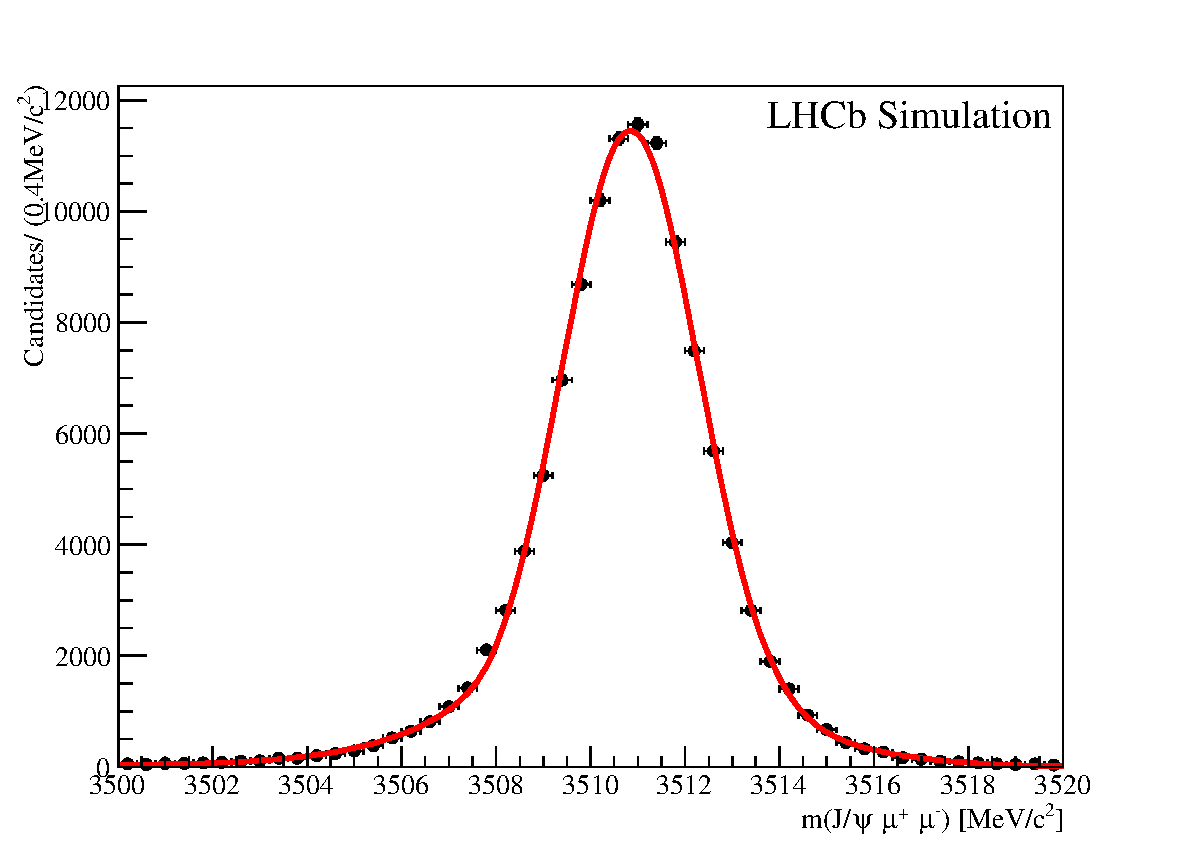
\includegraphics{figs/chic_1_GCB.pdf}}
%\vspace{-5mm}
\caption{\small  $J/\psi \mu^+ \mu^-$ invariant mass for the selected
  and truth matched $\chicone$ candidates in the simulation. }
\label{fig:gcb}
\end{center}
\end{figure}

To understand the relative importance of these contributions the
invariant mass is built using the Monte Carlo truth information together with  the
reconstructed momenta (slopes) of the
muons from the virtual photon and repeating the mass fit. The results
of this study are summarized in Table \ref{tab:rescontrib}. For this
decay mode, due to the low energy release, the most
important factor is the resolution on the track slopes. The contribution from the parameters of the mass constrained
particle, in this case the $J/\psi$, is small.
%
\begin{table}[htb!]
\caption{\small Contributions to the mass resolution for the $\chicone
  \rightarrow J/\psi  \mu^+ \mu^- $ decay mode. Reconstructed $p$
  the true slopes but reconstructed $p$ is used for the muon pair from
  the virtual photon. Reconstructed $tx,ty$ means the true $p$ but reconstructed $tx,ty$ is used for the muon pair from
  the virtual photon.  }
\begin{center}
\small
\begin{tabular}{l|c}
Condition & $\sigma [\mevcc]$   \\
\hline
Truth + Reconstructed $p$ & 0.9  \\
Truth + Reconstructed $tx,ty$ & 1.2\\
Truth + Reconstructed $p$ +Reconstructed $tx$ & 1.6 \\  
Fully reconstructed & 1.7 \\
\end{tabular}
\end{center}
\label{tab:rescontrib}
\end{table}

Furthermore, it can be seen from Fig. \ref{fig:sloperes} the application of the PV constraint improves the slope
resolution by a factor of two and
hence the mass resolution considerably \footnote{Qualitiatively this
  makes sense: adding the PV information provides a high precision
  measurement of the track position at its origin point and allowing
  to correct for any multiple scattering in the RF foil.}. This explains why the standard
release of  \textbf{RapidSim} which uses the unconstrained slope resolution
overestimates the mass resolution for these decays.
\begin{figure}[h!]
\centering
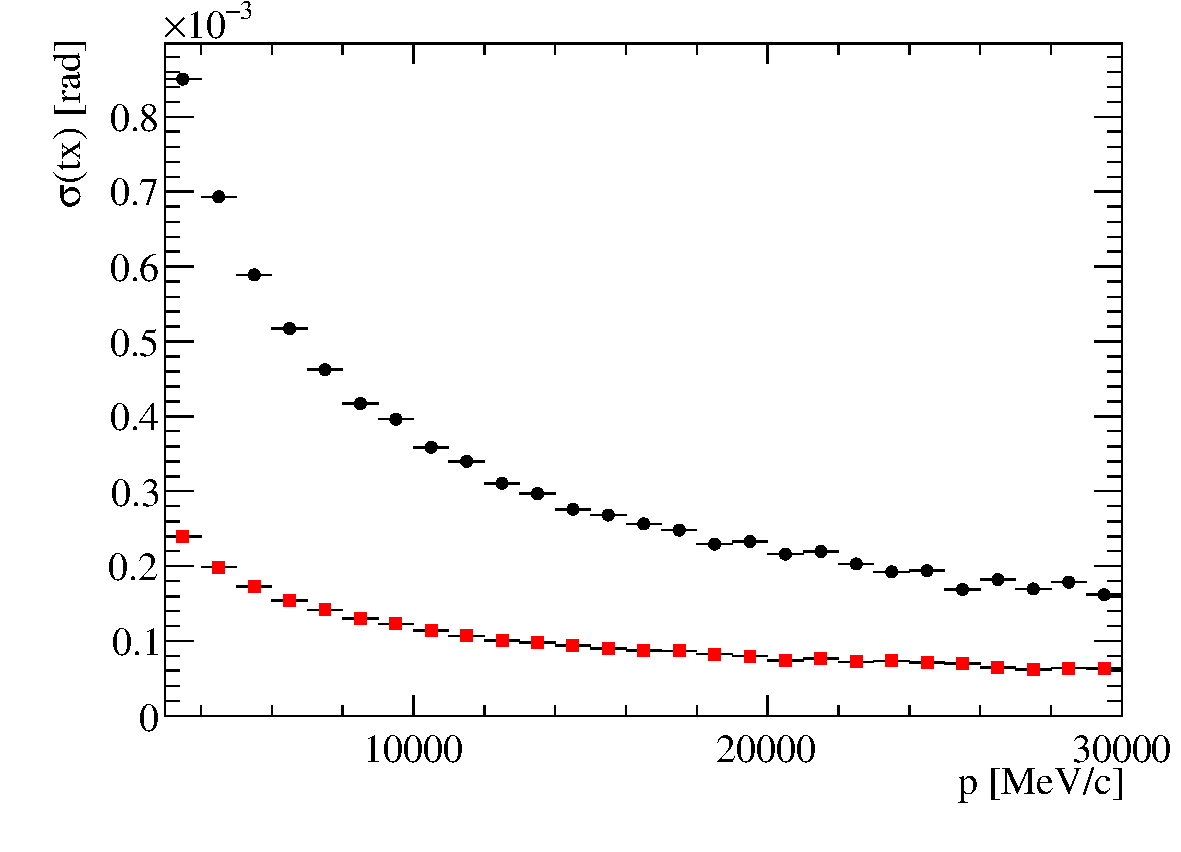
\includegraphics[width=0.48\textwidth]{figs/txres.pdf}
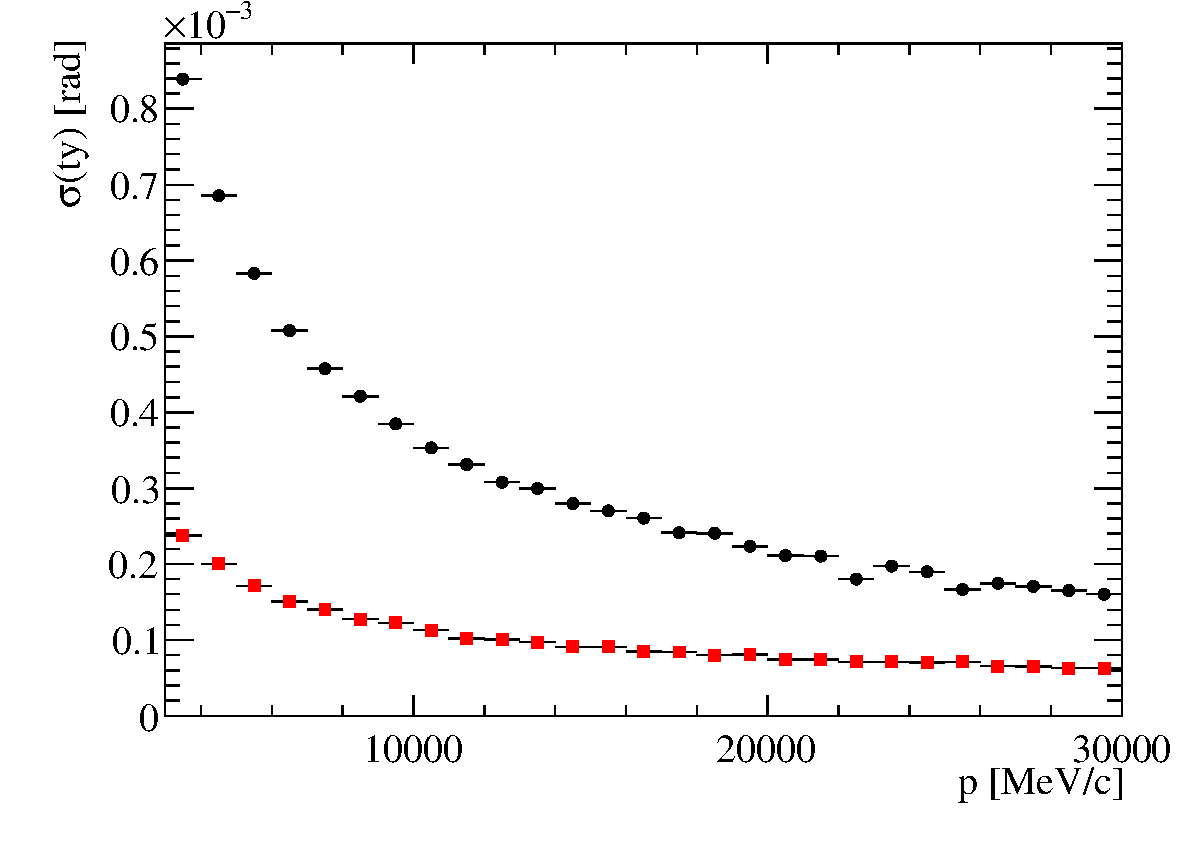
\includegraphics[width=0.48\textwidth]{figs/tyres.pdf}
\caption{(Left) Resolution on $tx$ versus $p$ before (black points) and after (red
  squares) the PV constraint is applied. (Right) Resolution on $ty$
  versus $p$ before (black points) and after (red
  squares) the PV constraint is applied for the muons from the virtual
  photon. In both cases the values are
  obtained by fitting a Gaussian to slices in $p$ to a 2-dimensional histogram.
   }
\label{fig:sloperes}
\end{figure}

To emulate the mass resolution the four-vectors of the muons and
$J/\psi$ are individually smeared, ignoring correlations. The parameterizations used for this
smearing are described in Section~\ref{sec:ep} - \ref{sec:res} and
takes into account the dependence of resolution on the particle kinematics. It will be
seen that this procedure reproduces the full simulation results well.

%\section{Parameterization of the magnet kick}
\label{sec:kick}
 %
As will be discussed in Section \ref{sec:ep} to model the momentum
resolution it is beneficial to use information on the track position after the magnet. \textbf{RapidSim}
has in place a single kick parameterization based upon the publicly
available studies described in
Ref.~\cite{VanTilburg:691686}. Based upon eye-balling this plot and taking
reasonable values for the track slopes before and after the magnet in
\textbf{RapidSim} a kick of $1.2 \gevc$ is applied at $z = 5.4 ~\textrm{m}$.  Since the referenced work
is rather old and the procedure to determine the kick parameters
rather coarse it was decided to redo this study. This leads to an
improved parameterization for use in \textbf{RapidSim}.

The magnet field parameterization is made using the  $\chicone \rightarrow J/\psi \mu^+ \mu^-$ and $\Upsilon(1S) \rightarrow
\mu^+ \mu^-$ simulation samples, selecting tracks from truth matched
candidates. To determine the effective magnetic
centre where the kick takes place the track state before and after the
magnet is needed. The track parameters before the magnet are easily
available from a \textbf{DecayTreeTuple}. A tool exists \footnote{TupleToolTrackPosition} to give
 the track position at given $z$. Storing the track $x$ and $y$ at $z
 = 9.2~\textrm{m} $ and $z
 = 10~\textrm{m}$ allows the track state after the magnet in a field
 free region to be estimated. From these two lines the intersection
 point at the magnet centre is easily calculated. This procedure is
 relatively crude but as will be seen gives a precision sufficient
 for these studies \footnote{It would be better to us MC truth both
   before and after the magnet. However, the latter information is not
 stored on the DST.}. Fig.~\ref{fig:zc} shows the
 distribution of the calculated magnet centre. The mode of this
 distribution ($z_c = 5.26 \textrm{m}$) is taken as the magnet centre
 \footnote{It is known that $z_c$ depends on the tracks kinematics but
   for the accuracy needed here a single value is
   considered sufficient. }.
\begin{figure}[htb!]
\begin{center}
\resizebox{4.0in}{!}{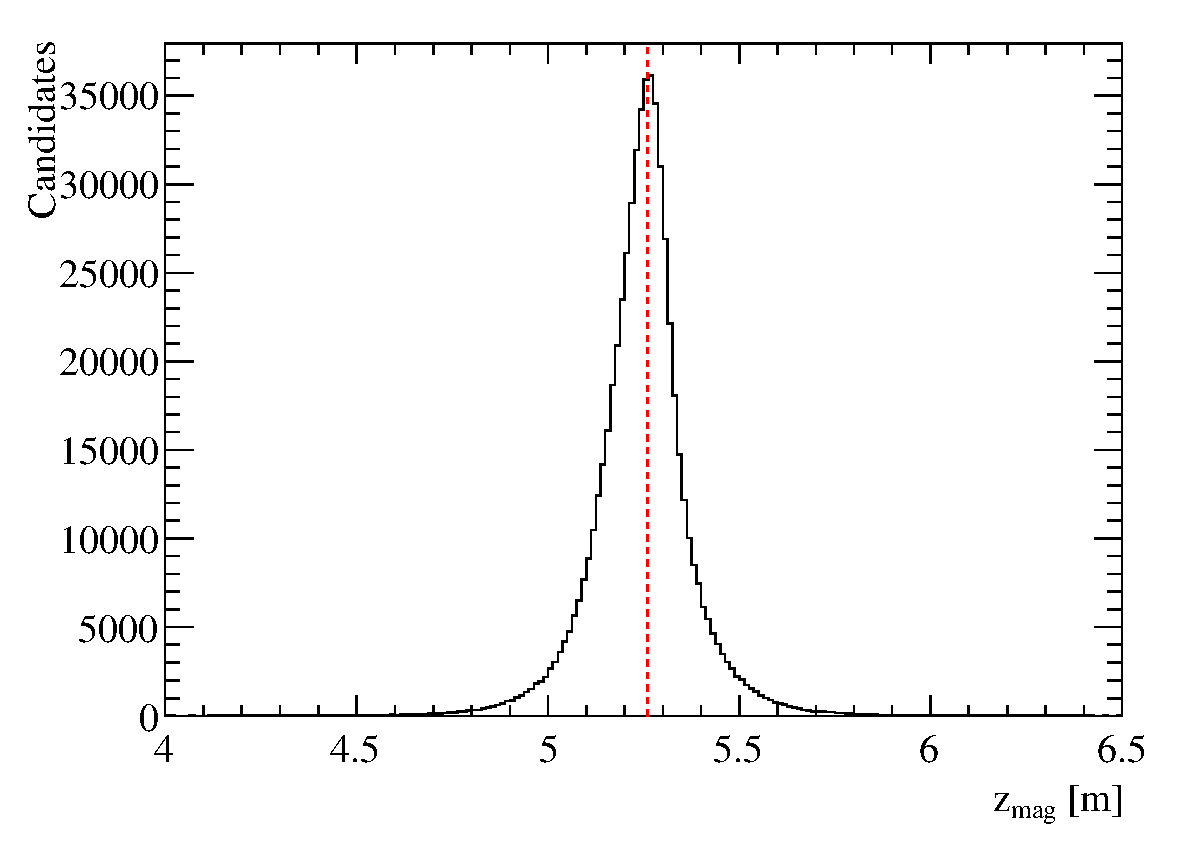
\includegraphics{figs/zc.pdf}}
\caption{\small Distribution of the estimated magnet centre calculated
  using tracks from the $\chicone$ and $\Upsilon$ samples. The
  dotted red line shows the mode of the distribution $z_c = 5.26~\textrm{m}$. }
\label{fig:zc}
\end{center}
\end{figure}

From the studies in  Ref.~\cite{VanTilburg:691686} is it known the
size of the kick of the magnet increases with $ty$. This can be seen
in Fig.~\ref{fig:by} where the $\pt$ kick of the magnet is plotted
versus $ty$. As in the previous study is found that this shape can be
modelled with a second-order polynomial.
\begin{figure}[htb!]
\begin{center}
\resizebox{4.0in}{!}{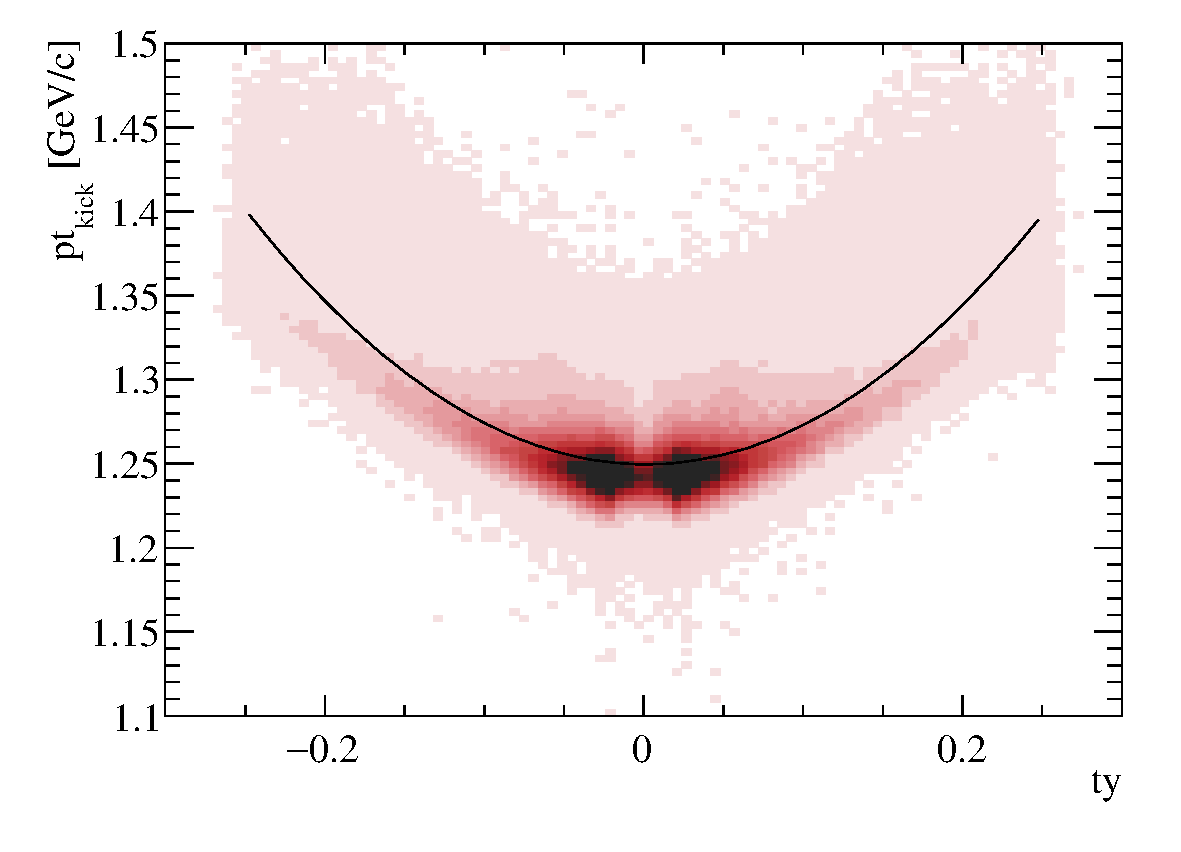
\includegraphics{figs/by.pdf}}
\caption{\small $\pt$ kick versus $ty$. A fit to a second order
  polynomial is superimposed. The coefficients of the polynomial are $1.25
  \gevc$, $-0.006~\gevc$ and $2.45~\gevc$. }
\label{fig:by}
\end{center}
\end{figure}

Fig.~\ref{fig:dx} shows the difference between the x-position
calculated by the track fit at $z = 9.2~\textrm{m}$ and the single-kick
parameterization above. The RMS of the distribution is $0.8 ~\textrm{cm}$
which is adequate for our needs. Performing the same exercise
in $y$ (where the only effect is multiple scattering) gives a precision of $0.5~\textrm{cm}$. This means that
the precision of the parameterization is around $0.6 \textrm{cm}$. 

An interesting question is the gain in precision compared to the
parameterization currently used in \textbf{RapidSim}. Using that the
RMS of the distribution is broadened to $1.5~\textrm{cm}$ and there is
a clear double peak structure reflecting the fact the parameterization
leads a to a bias of $1~\textrm{cm}$ for each charge (Fig.\ref{fig:dxsimple}). Clearly the new
parameterization is better though all things considered the old
parameterization was not so bad.
%
\begin{figure}[htb!]
\begin{center}
\resizebox{4.0in}{!}{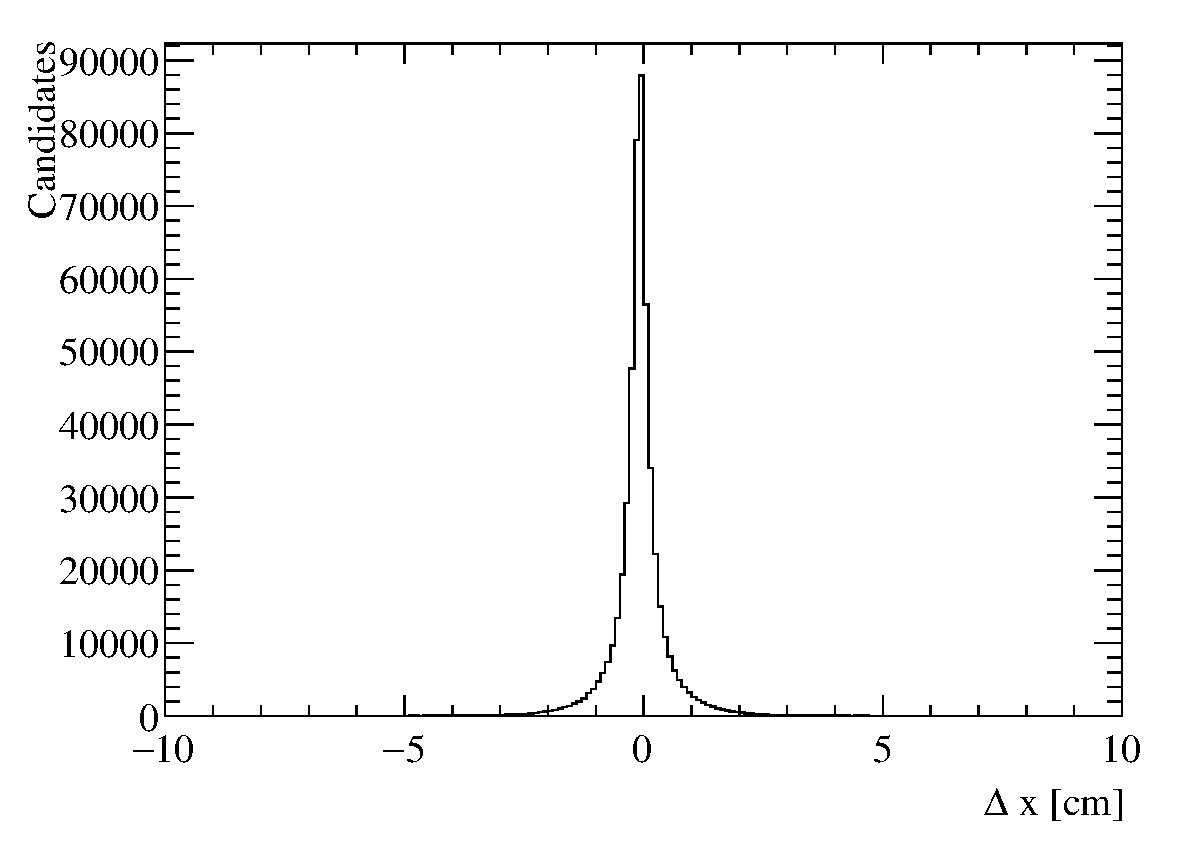
\includegraphics{figs/dx.pdf}}
\caption{\small Difference between the x-position
calculated by the track fit at $z = 9.2~\textrm{m}$ and the single-kick
parameterization.}
\label{fig:dx}
\end{center}
\end{figure}
%
\begin{figure}[htb!]
\begin{center}
\resizebox{4.0in}{!}{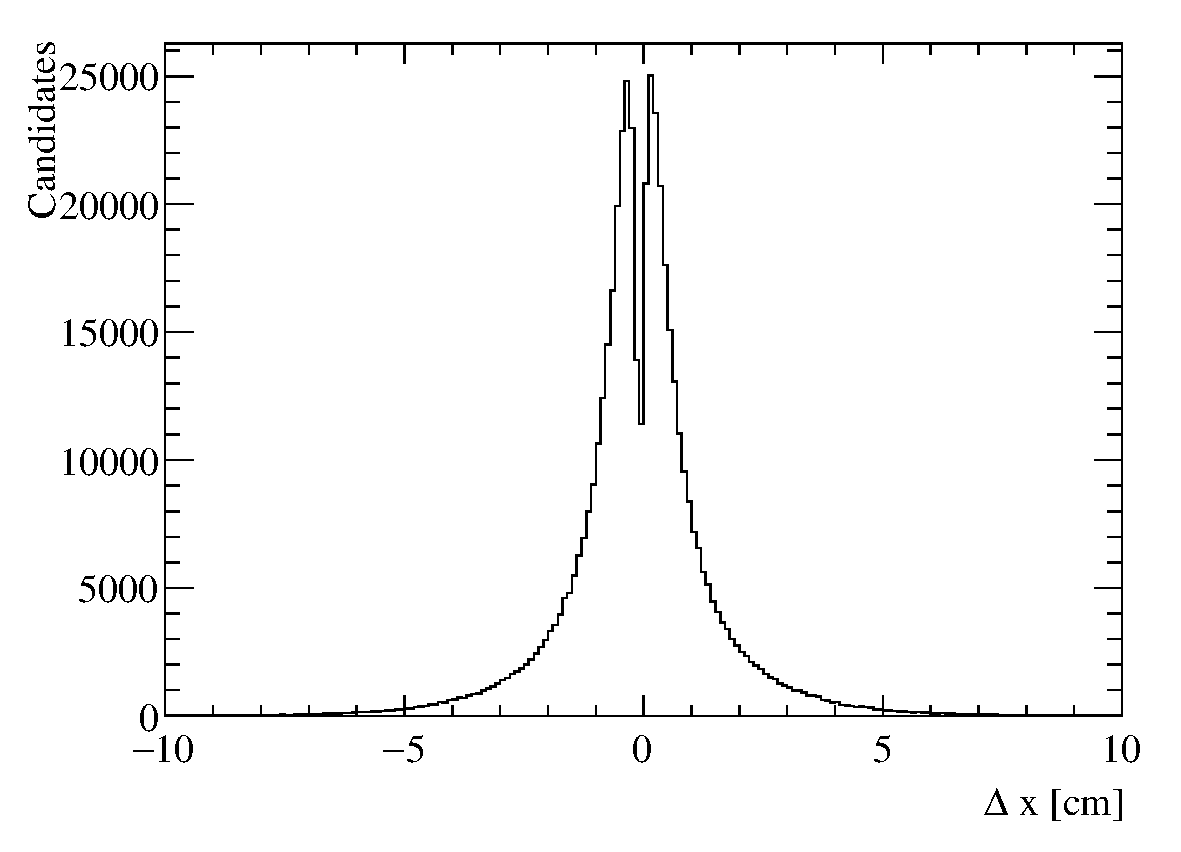
\includegraphics{figs/simple.pdf}}
\caption{\small Difference between the x-position
calculated by the track fit at $z = 9.2~\textrm{m}$ and the default single-kick
parameterization in \textbf{RapidSim}.}
\label{fig:dxsimple}
\end{center}
\end{figure}
%

\section{Momentum Resolution}
\label{sec:ep}
 %
To parameterize the smearing due to the momentum resolution the
estimate of the momentum uncertainty provided by the Kalman track fit
is used since it is known to be reliable at the level of $10 \%$ or better.  

%
The LHCb spectrometer is rather complex and consequently the momentum
resolution depends on individual track kinematics. This can be seen in
Fig.  \ref{fig:eppfit} where the calculated uncertainty on the momentum from the
track fit ($\sigma^{fit}_{p}$) divided by $p$ is plotted versus $p$ for tracks from the
$\chicone \rightarrow J/\psi \mu^+ \mu^-$ and $\Upsilon(1S) \rightarrow
\mu^+ \mu^-$ samples. Three regions with different performance have been marked with dashed lines:
\begin{description}
\item[IT] These tracks pass through
  the acceptance of the Inner Tracker and consequently benefit from
  its good hit resolution.
\item[OT] These tracks pass through the Outer Tracker which has worse
  hit resolution compared to the Inner Tracker.
\item[High $\eta$] The origin of the worse momentum resolution for this region
  has several causes. Tracks in this region lie at high $\eta$, close to
  the edge of the detector acceptance. They are likely to have no
  information in TT and relatively few VELO hits which worsens the
  resolution. It also seems at least some of these tracks are deflected
  by the magnetic field through the beam-pipe which signficantly worsens their
  momentum resolution since they traverse alot of material
  \footnote{The track sample used contains only muons which are only
    effected by multiple scattering and do not interact hadronically.}. 
\end{description}
%
\begin{figure}[htb!]
\begin{center}
\resizebox{5.0in}{!}{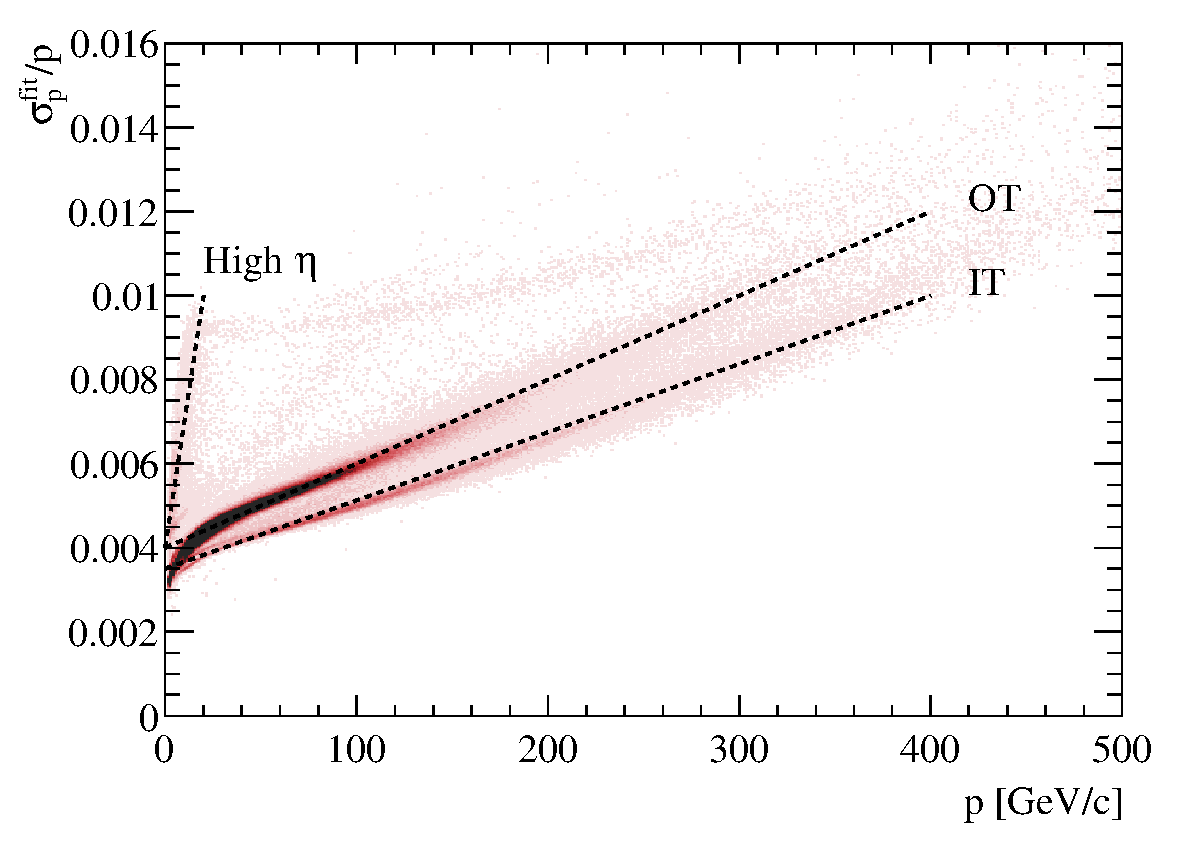
\includegraphics{figs/epp-fit.pdf}}
\caption{\small $\sigma^{fit}_{p}$ versus $p$ for the combined
  $\chicone$ and $\Upsilon$ track sample. }
\label{fig:eppfit}
\end{center}
\end{figure}

For use in a fast simulation these details need to be captured. 
This is a straightforward regression problem with the
input variables being the track kinematics and the target being the
value of $\sigma^{fit}_{P}$ estimated from the track fit. To do this a
Gradient Boosted Decision\footnote{Other methods, e.g. a neural
  network, gave similar results but were more CPU intensive.} tree from the TMVA package \cite{Hocker:2007ht} was
used with the following input variables:
\begin{description}
\item[$\mathbf{p}$] Momentum
\item[$\mathbf{tx}$] Slope in x-direction
\item[$\mathbf{ty}$] Slope in y-direction
\item[$\boldsymbol{\eta}$] pseudorapidity
\item[$\boldsymbol{\phi}$] azimuthal angle
\item[$\mathbf{\pt}$] Transverse momentum
\item[$\mathbf{q\times pol}$] Charge times magnet polarity
%\item[$\mathbf{x_T}$] x position at $9200$ cm 
%\item[$\mathbf{y_T}$] y position at $9200$ cm
\end{description}
The idea of giving both the $(p,tx,ty)$ and $(\pt,\eta,\phi)$
representation is that the detector has some structures (e.g detector
boxes) that are best captured by the first representation and some
(e.g. the 25 mrad cone of the beam-pipe) that are best captured by the
second. 

%The use of the information on the track position in the T-stations
%was found to more accurately capture the high $\eta$ structure in
%Fig. \ref{fig:eppfit}. To calculate $x_T$ and $y_T$ the parameterization
%given in Section~\ref{sec:kick} is used. 
For training the  $\chicone \rightarrow \jpsi \mu^+ \mu^-$ and $\Upsilon(1S) \rightarrow
\mu^+ \mu^-$ samples are used. This allows to cover the full momentum
range of the spectrometer from $3-500 \gevc$ meaning the applicability of this BDT is
wider than the scope of this study. The most highly ranked variables
were $p$, $\eta$ and $\pt$. The performance of the BDT
estimator is good as can be seen from Fig. \ref{fig:corel} and
\ref{fig:diff}. The relative accuracy of the method is $\sim 2.8 \%$
(RMS of Fig. \ref{fig:diff} (Right)) and
it captures the most features of the target distribution well. The
main discrepancy visual is that the long-tail in the high $\eta$ region is
not well reproduced. 
%
\begin{figure}[h!]
\centering
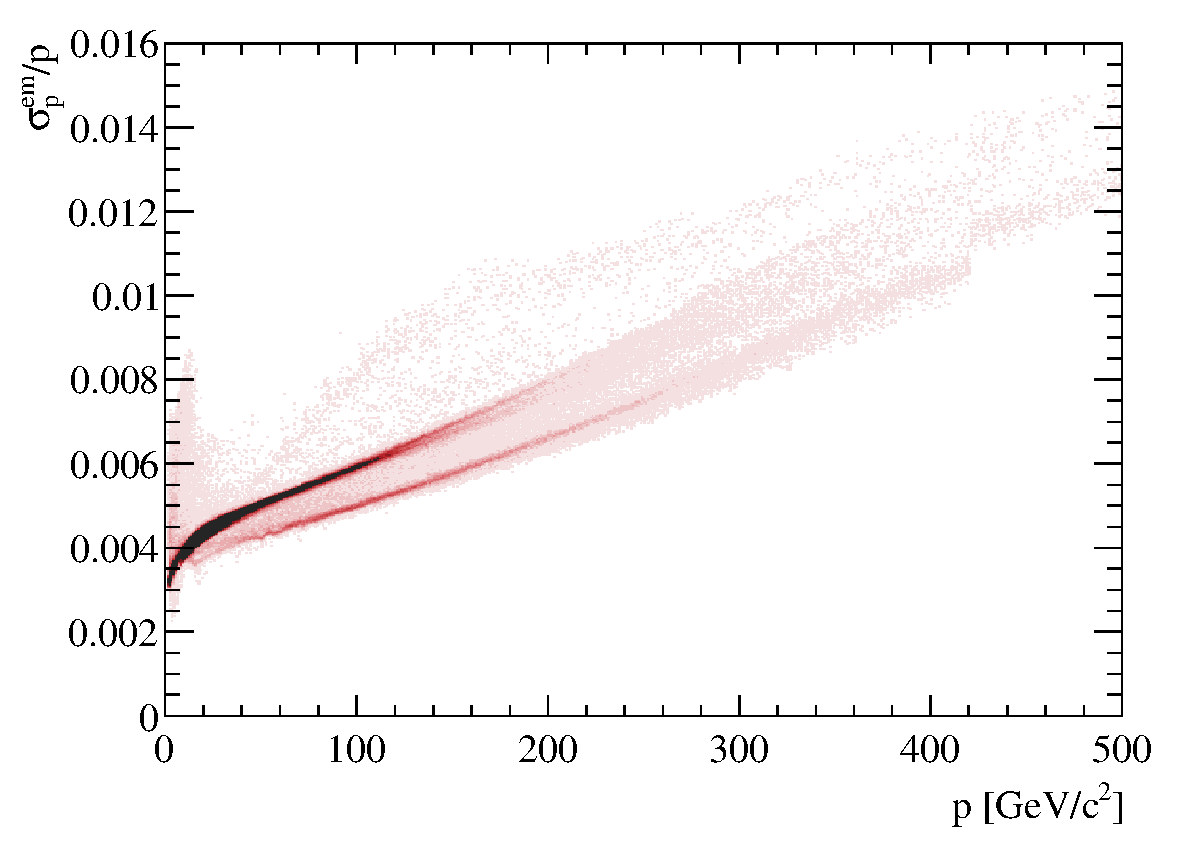
\includegraphics[width=0.48\textwidth]{figs/epp-em.pdf}
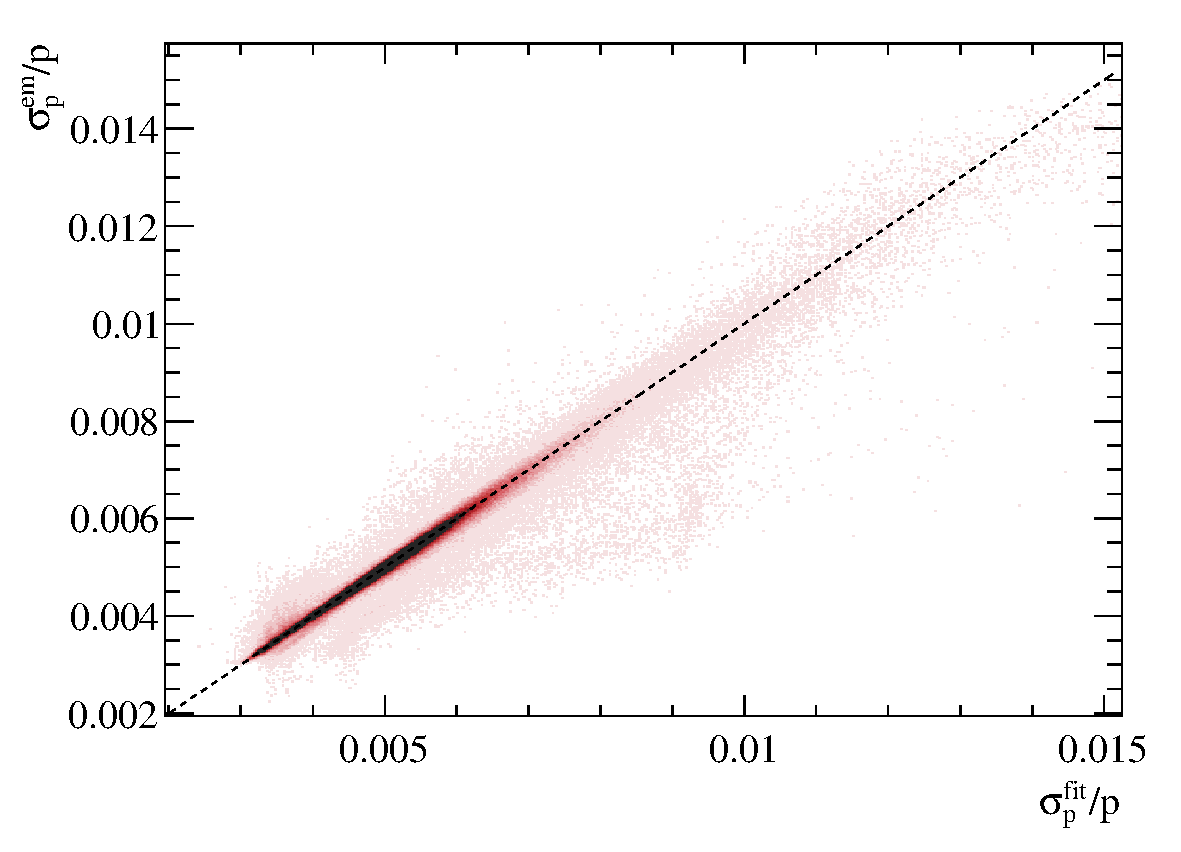
\includegraphics[width=0.48\textwidth]{figs/corelation.pdf}
\caption{(Left) $\sigma^{em}_{p}$ versus $p$ and (Right)
  $\sigma^{em}_{p}$  versus  $\sigma^{fit}_{p}$. The dotted line
  corresponds to perfect corelation. Both plots are made with the combined
  $\chicone$ and $\Upsilon$ sample.  }
\label{fig:corel}
\end{figure}
%
\begin{figure}[h!]
\centering
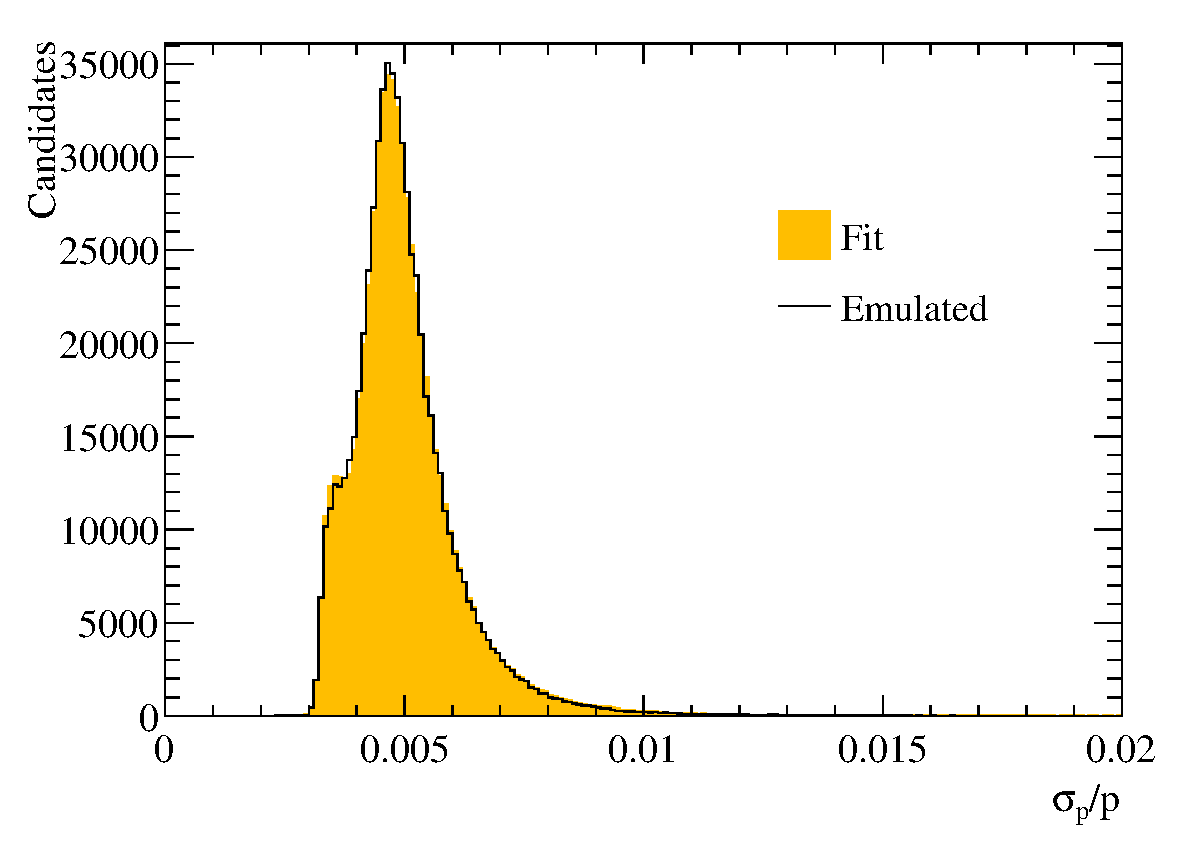
\includegraphics[width=0.48\textwidth]{figs/ep.pdf}
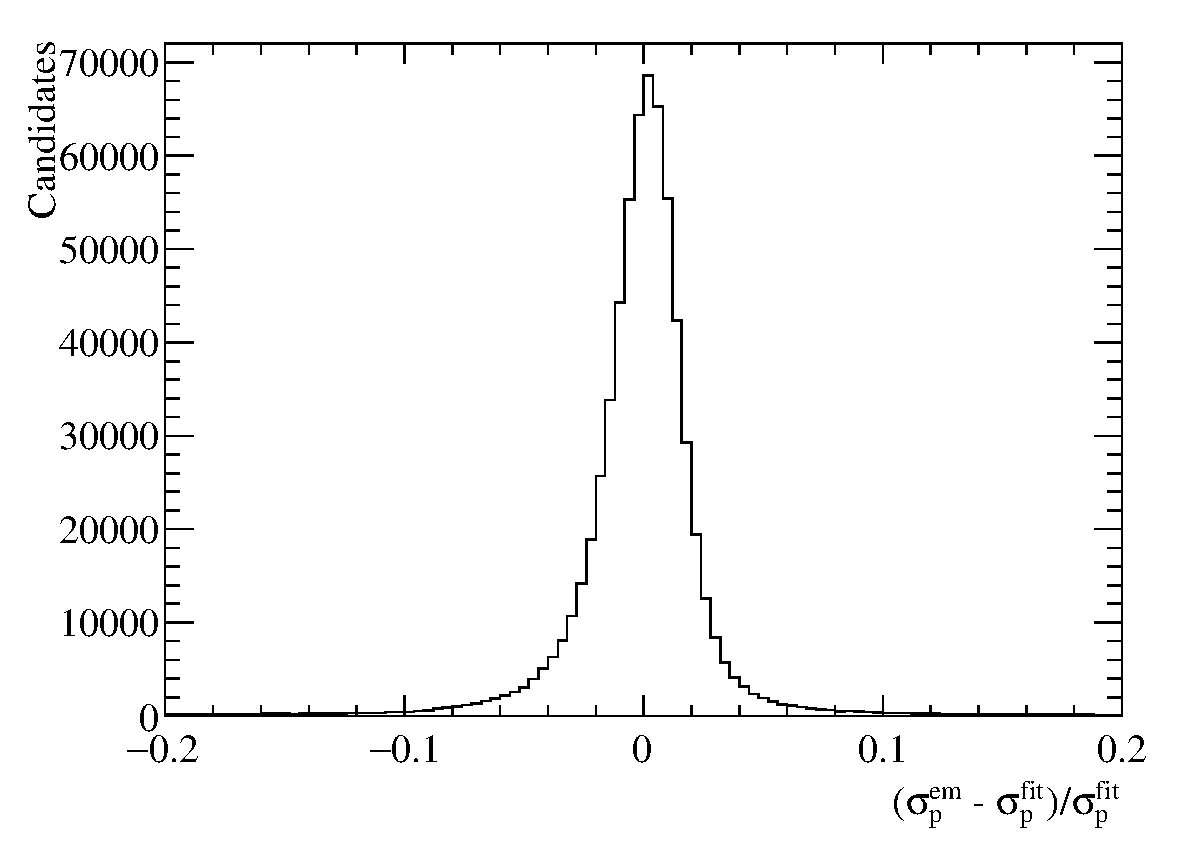
\includegraphics[width=0.48\textwidth]{figs/difference.pdf}
\caption{(Left) Distribution of $\sigma^{em}_{p}$ and
  $\sigma^{fit}_{p}$. The shape of this distribution reflects the
  input samples used for training. (Right) Distribution of the relative difference between $\sigma^{em}_{p}$ and
  $\sigma^{fit}_{p}$  }.
\label{fig:diff}
\end{figure}

The quality of this estimate can be judged from the pull, defined as 
\begin{equation*}
\frac{p_{rec} - p_{true}}{\sigma^{em}_{p}}.
\end{equation*}
Figure \ref{fig:ppull} shows the resulting pull distribution. The RMS of this
distribution is 1.2. The tails are expected and due to the fact that there are
non-Gaussian tails in the energy loss and multiple scattering
processes that are not captured by the Kalman filter. Fitting a double
Gaussian gives a central core with a width 0.93 and a wider Gaussian
with width 1.9. The fraction in the core is $92 \%$. It is easy to
incoporate these values into the emulator by using double Gaussian
smearing.  The pull distribution
also exhibits a small bias (0.09), probably due to the tail in the energy loss
distribution. This bias is ignored for the emulation \footnote{The
  momentum scale in the full simulation is known to need tuning. For
  the use case envisaged of $\chi_{b}$ Dalitz decays the momentum
  scale on data is readily cross-checked with other modes.}.
%
\begin{figure}[htb!]
\begin{center}
\resizebox{3.8in}{!}{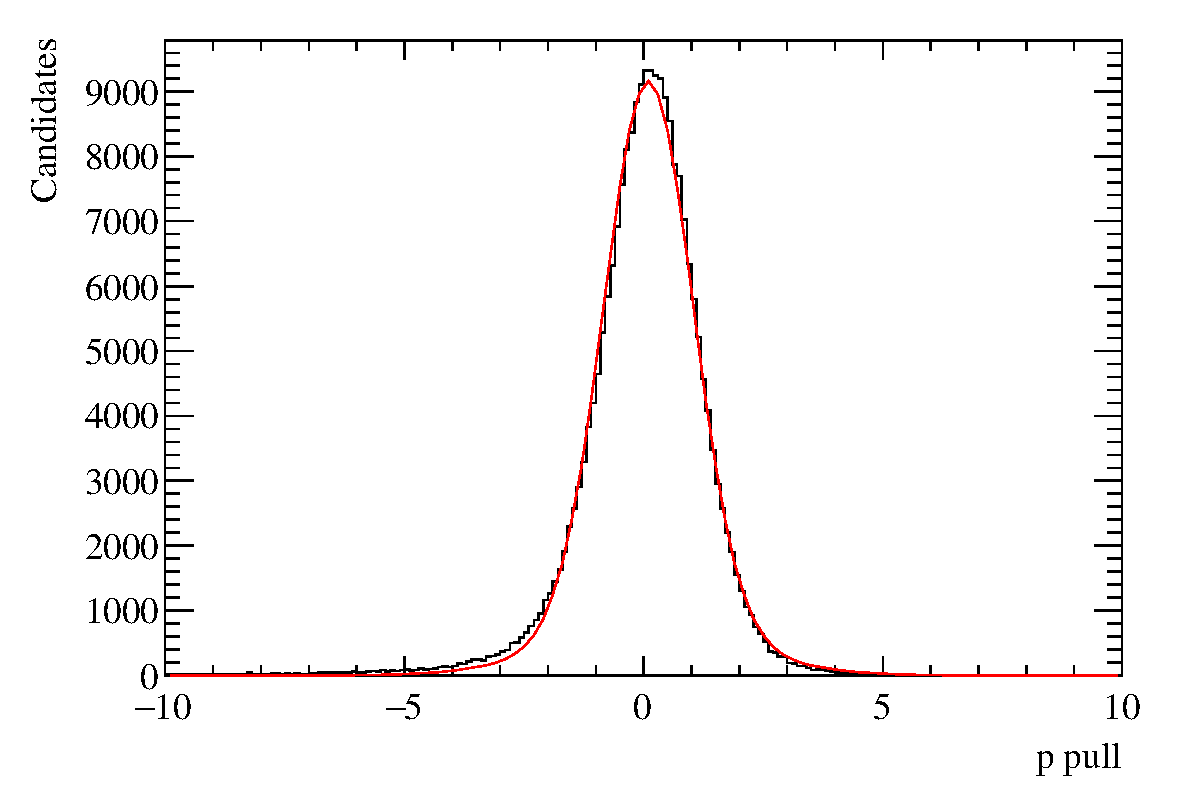
\includegraphics{figs/pullp.pdf}}
\caption{\small Momentum pull using the emulation. A fit to a double
  Gaussian function is superimposed.}
\label{fig:ppull}
\end{center}
\end{figure}


\section{Track slopes}
\label{sec:slopesmva}
%
An MVA approach was also used to parameterize the uncertainty on the
track slopes. Again the \textbf{BDTG} method from the \textbf{TMVA}
package was used. The input variables were $p$, $\eta$, $\pt$, $\phi$,
$tx$ and $ty$. The highest ranked variables are $p$, $\eta$ and $\phi$
in that order. For training the signal tracks from the virtual photon
$\chicone \rightarrow J/\psi \mu^+ \mu^-$ sample are used. Separate
BDTs are trained for the uncertainites in $tx$ and $ty$.

Figure \ref{fig:coreltx} (Figure \ref{fig:corelty}) shows the correlation between the track fit and emulated
value of uncertainty the relative differecne on $tx$ ($ty$). The
distributions of the fit and emulated values are shown in Fig. ~\ref{fig:etxty}. The fitted
and emulated values agree at the level of $10 \%$ with some
tail. Comparisons of the emulated and fit values of $p$, $\phi$ and
$\eta$ are given in Appendix~\ref{sec:slopeplots}. 
%
\begin{figure}[h!]
\centering
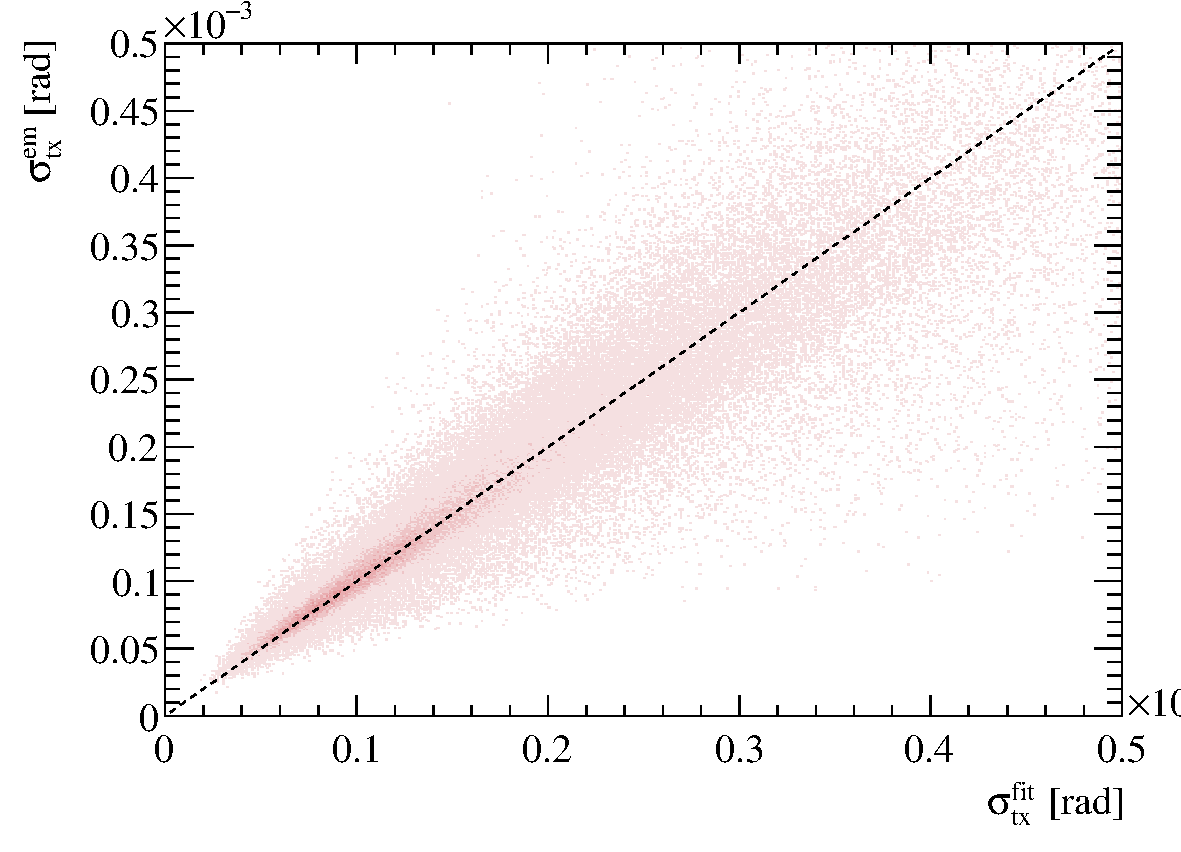
\includegraphics[width=0.48\textwidth]{figs/corelation-tx.pdf}
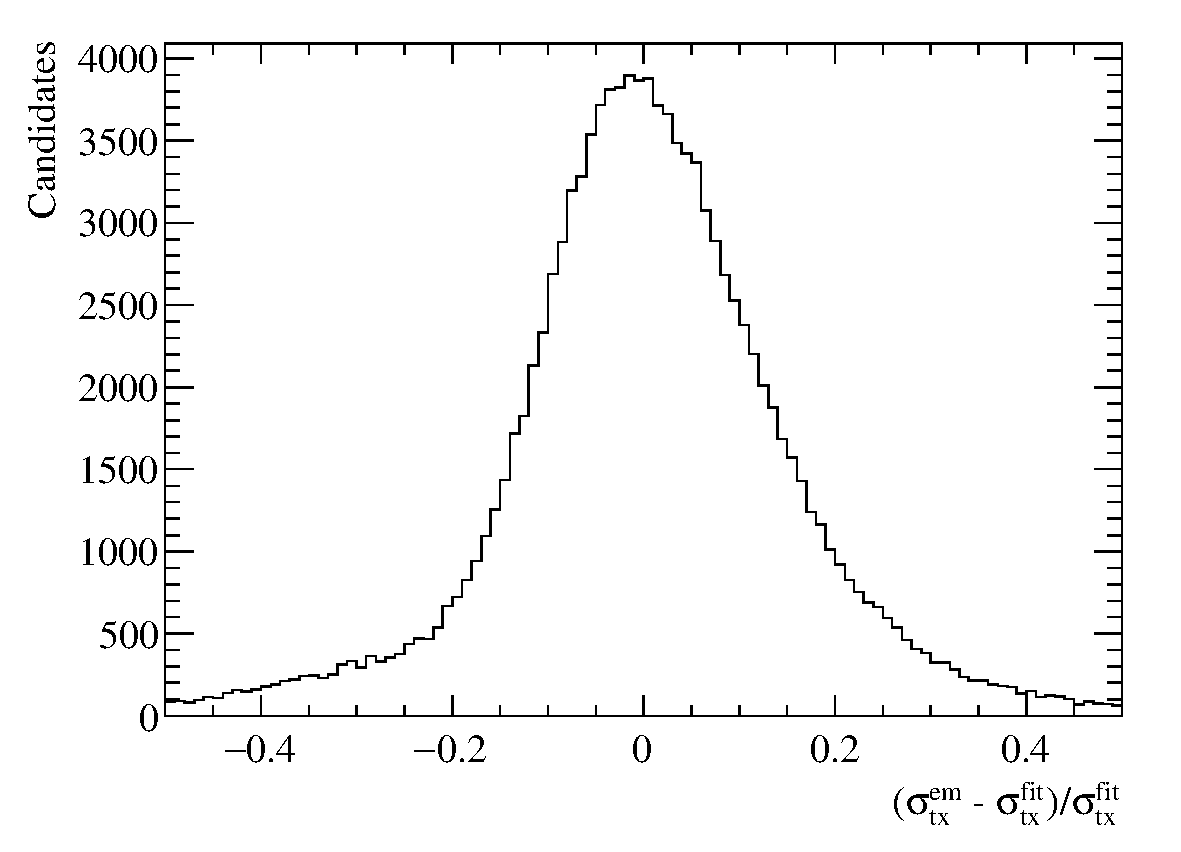
\includegraphics[width=0.48\textwidth]{figs/difference-tx.pdf}
\caption{(Left)  $\sigma^{em}_{tx}$  versus  $\sigma^{fit}_{tx}$. The dotted line
  corresponds to perfect corelation. (Right) Relative difference
  between $\sigma^{em}_{tx}$  and  $\sigma^{fit}_{tx}$.}
\label{fig:coreltx}
\end{figure}
%
%
\begin{figure}[h!]
\centering
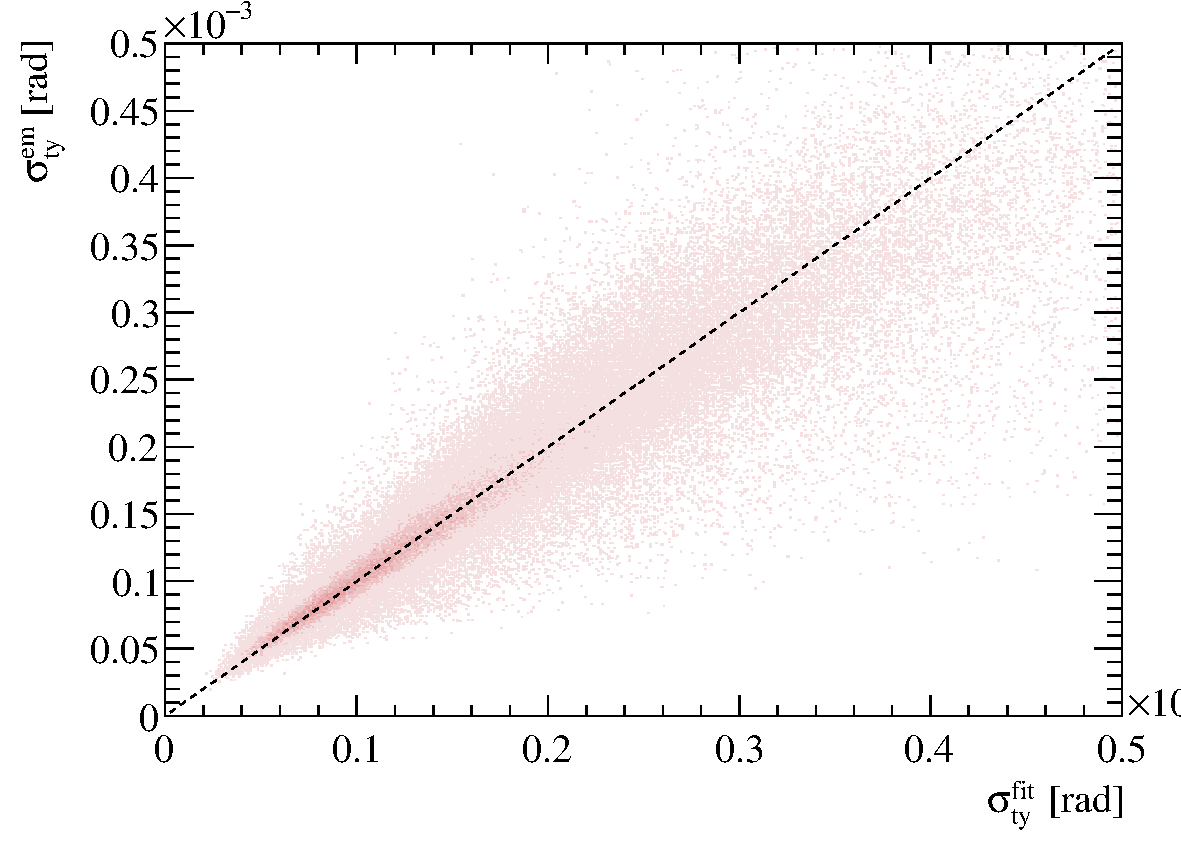
\includegraphics[width=0.48\textwidth]{figs/corelation-ty.pdf}
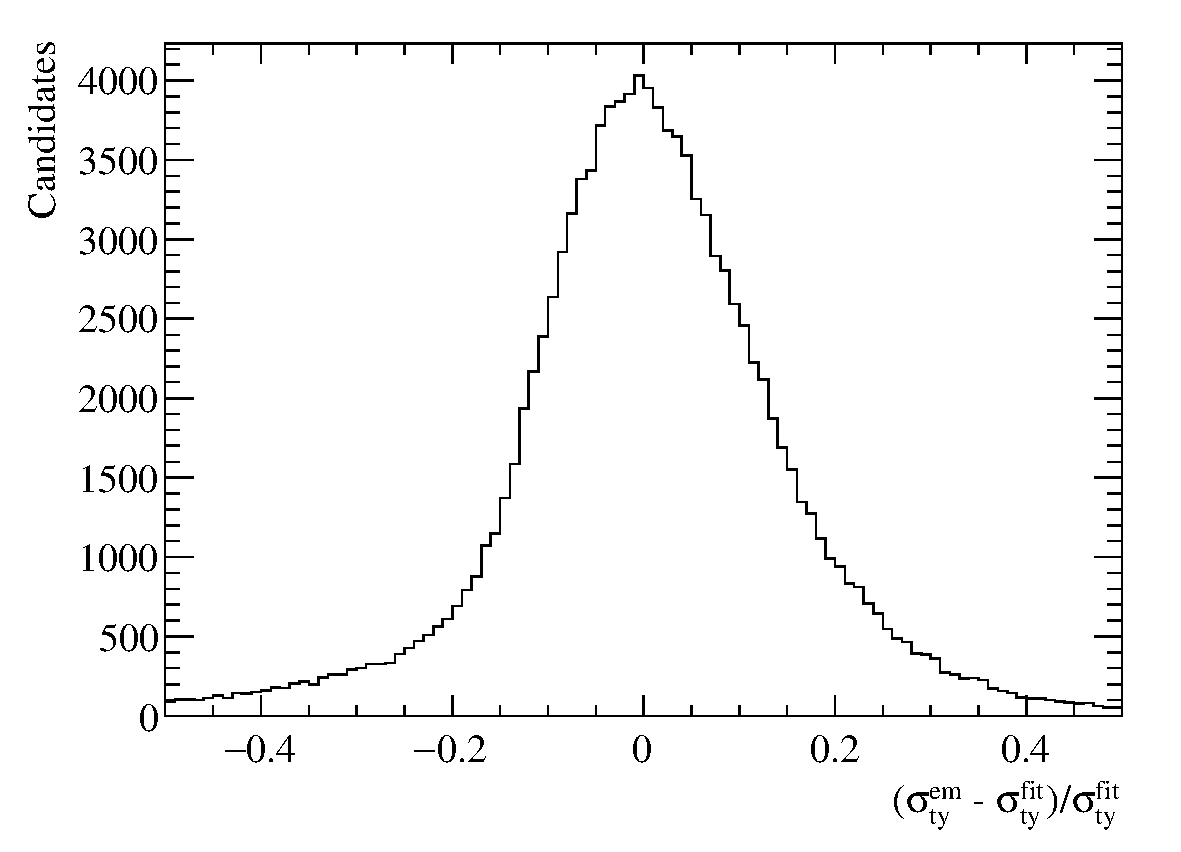
\includegraphics[width=0.48\textwidth]{figs/difference-ty.pdf}
\caption{(Left)  $\sigma^{em}_{ty}$  versus  $\sigma^{fit}_{ty}$. The dotted line
  corresponds to perfect corelation. (Right) Relative difference
  between $\sigma^{em}_{ty}$  and  $\sigma^{fit}_{ty}$.}
\label{fig:corelty}
\end{figure}
%
\begin{figure}[h!]
\centering
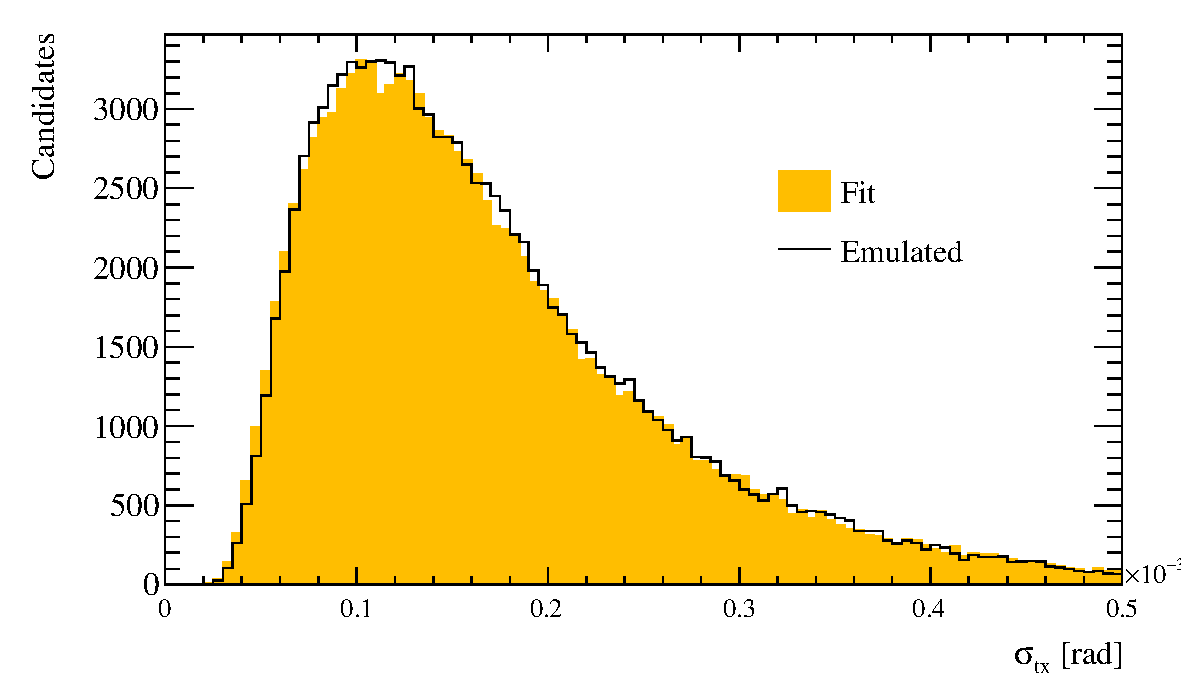
\includegraphics[width=0.48\textwidth]{figs/etx.pdf}
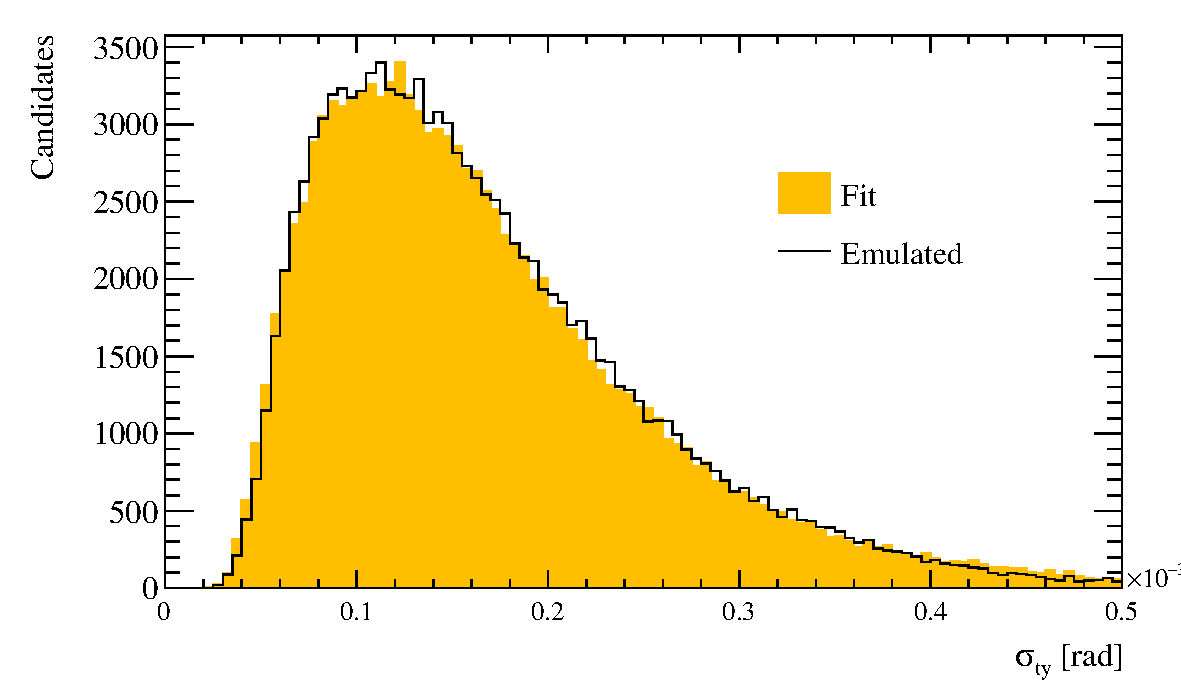
\includegraphics[width=0.48\textwidth]{figs/ety.pdf}
\caption{(Left)  Emulated and fit values of the uncertainty on $tx$
  and (Right) Emulated and fit values of the uncertainty on $ty$. }
\label{fig:etxty}
\end{figure}
%

%
The quality of the estimated uncertainties is judged from the
pulls. The RMS of this
distribution is 1.25. Fitting a double
Gaussian gives a central core with a width 0.91 and a wider Gaussian
with width 2. The fraction in the core is $90 \%$. It is easy to
incoporate these values into the emulator by using double Gaussian
smearing.  

An approach to emulating the uncertainties on $tx$ and $ty$ using a
parametric form was also developed but abandoned as it was found not
to work as well as the MVA approach. For completeness the results of
those studies are given in Appendix~\ref{sec:slopes}.

\section{Resonance resolution}
\label{sec:res}
% 
The final component of the mass resolution is due to the uncertainties
on the parameters of the $J/\psi$ resonance. This component is
relatively small ($0.6 \mevc$ for the $\chicone$ decay given the
numbers in Table \ref{tab:rescontrib}) due to the mass constraint applied in the kinematic
fit. A similar approach is adopted as for the track slopes. That is to
fit the difference between the true and reconstructed values of the
$J/\psi$ slopes and momentum in slices and parameterize the
result. For the slopes the form give in Equation \ref{eq:sloperes}, with $A_{res} = 2.9 \times 10^{-5}$ and $B_{ms} =
7.5 \mevc$, is found to fit well (Fig. \ref{fig:resty}).  
%
\begin{figure}[htb!]
%\vspace{-5mm}
\begin{center}
\resizebox{3.5in}{!}{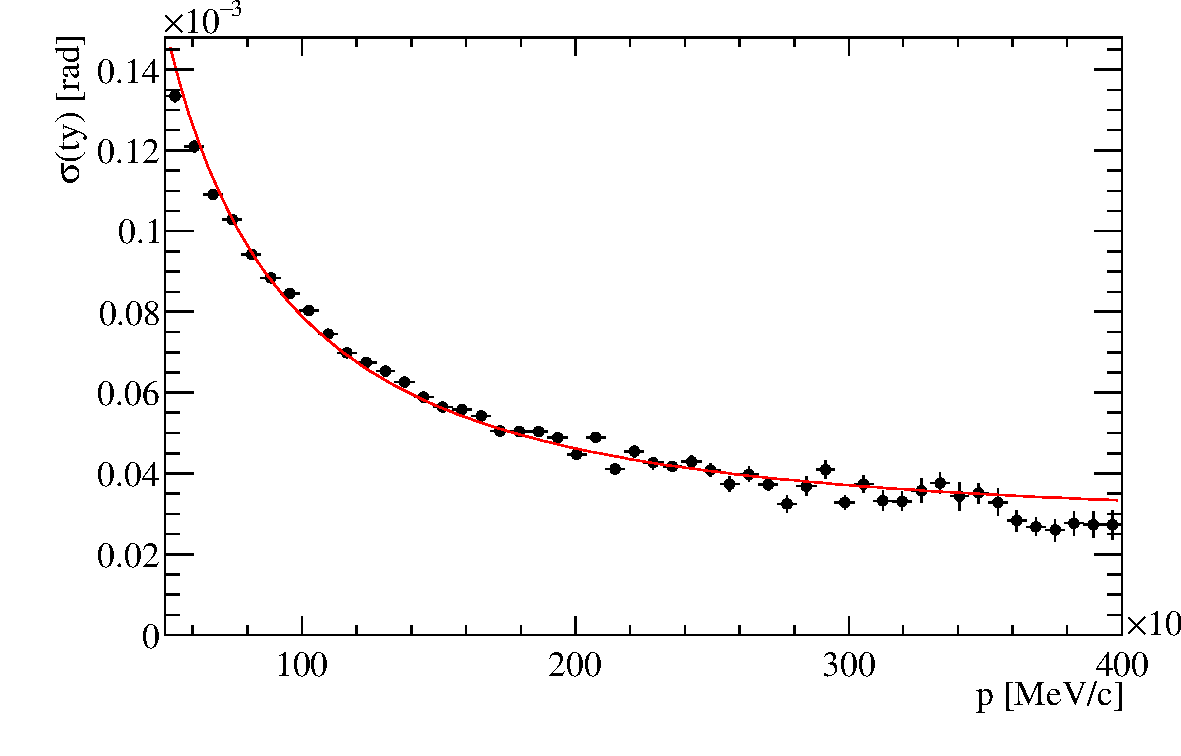
\includegraphics{figs/resty.pdf}}
%\vspace{-5mm}
\caption{\small Resolution on the $J/\psi$ slope in $ty$. A fit to the
  form discussed in the text is superimposed.} 
\label{fig:resty}
\end{center}
\end{figure}

For the uncertainty from the $J/\psi$ momentum no aesthetically pleasing
parameterization is found (Fig. \ref{fig:resp}) and the distribution is
modelled with a $4^{th}$ order polynomial.

\begin{figure}[htb!]
%\vspace{-5mm}
\begin{center}
\resizebox{3.5in}{!}{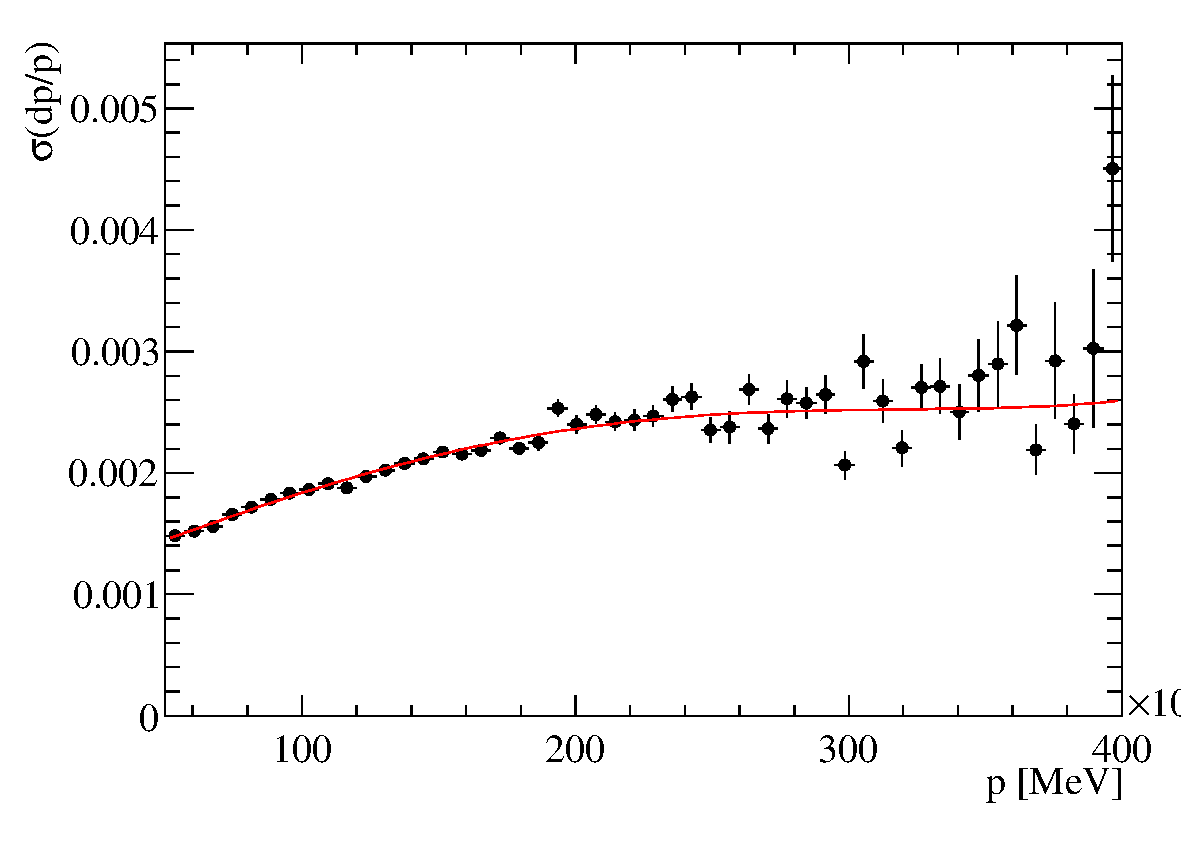
\includegraphics{figs/resp.pdf}}
%\vspace{-5mm}
\caption{\small Resolution on the $J/\psi$ momentum as function of
  momentum. A fit to a fourth order polynomial is superimposed. The
  polynomial parameters (with $p$ in $\mevc$) are $1 \times 10^{-3}, 7
\times 10^{-9}, 1 \times 10^{-14}, -1.2 \times 10^{-19}, 1.7 \times 10^{-25} $. }
\label{fig:resp}
\end{center}
\end{figure}


\section{Validation}
\label{sec:validation}
%
Figure ~\ref{fig:mplot} shows the $\Delta m= m^{fit}(\jpsi \mu^+ \mu^-)
- m^{em}(\jpsi \mu^+ \mu^-)$ distribution \footnote{Plotting $\Delta m$
  removes the effect of radiative corrections.   } for the $\chicone
\rightarrow J/\psi \mu^+ \mu^-$  decay mode obtained with the full
simulation and the emulator. It can be seen the agreement  is good
(allowing for a small shift). The emulator describes the core of the
distribution well but slightly underestimates the tail.
%
%
\begin{figure}[htb!]
\begin{center}
\resizebox{3.8in}{!}{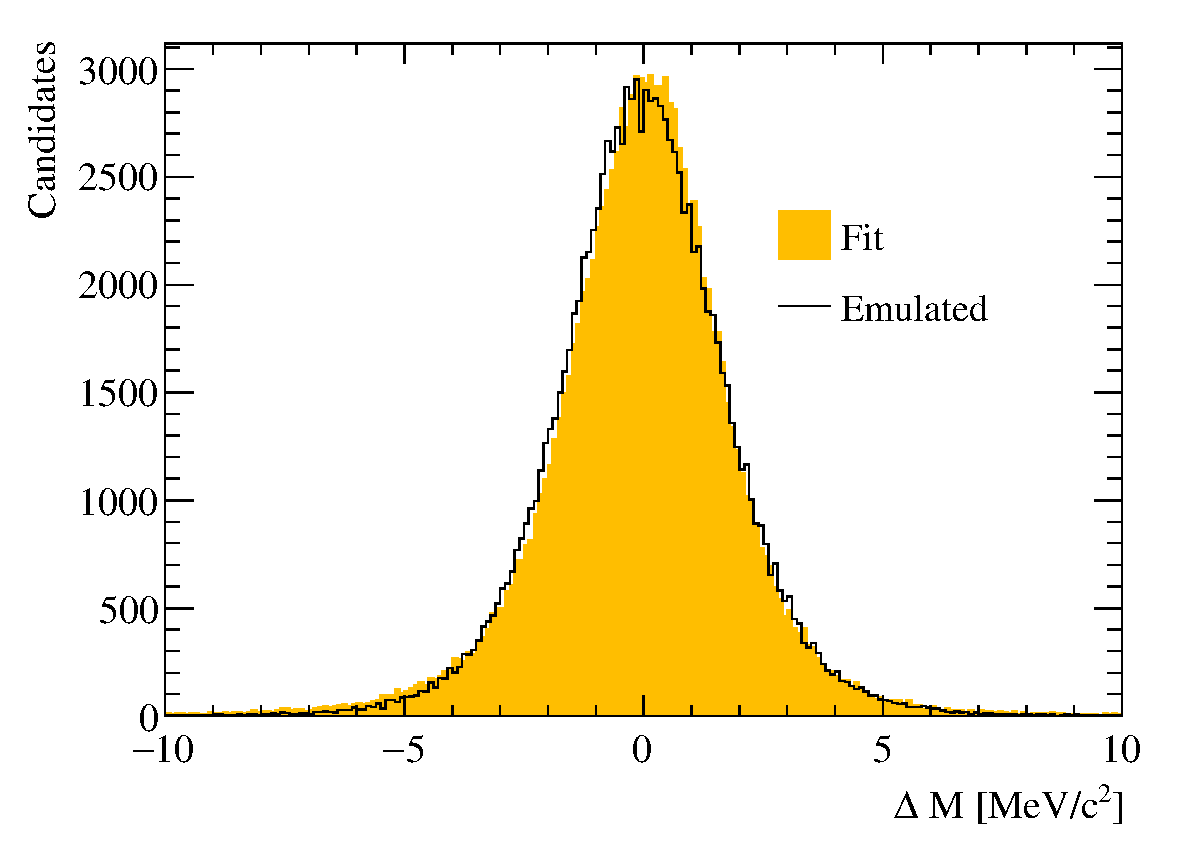
\includegraphics{figs/mplot.pdf}}
\caption{\small  Comparison of the mass resolution for the  $\chicone
\rightarrow J/\psi \mu^+ \mu^-$  decay mode with the full simulation
and the emulator. }
\label{fig:mplot}
\end{center}
\end{figure}

The quality of the emulator has been judged in two ways. First, for
the 
$\chicone \rightarrow J/\psi \mu^+ \mu^-$  decay mode the resolution
found with the full simulation and emulator using the fit model
described in Section~\ref{sec:chic} are compared as function
of the virtual photon momentum ($p_{pair}$), the candidate $\pt$ and
rapidity ($y$) in Figs.~\ref{fig:sigmappair} - \ref{fig:sigmay}. The
emulator correctly describes the trends seen with the full simulation
and the agreement is at the level of $5 \%$ or better apart from at high
$\chi_{c1}$ transverse momentum where the agreement is at the level of
$8 \%$. The disagreement at high $\pt$ is a common feature of all the
modes considered (Table \ref{tab:valid10}). This is an important
observation for the use case of using the emulator on other modes. 

%
\begin{figure}[htb!]
\begin{center}
\resizebox{3.8in}{!}{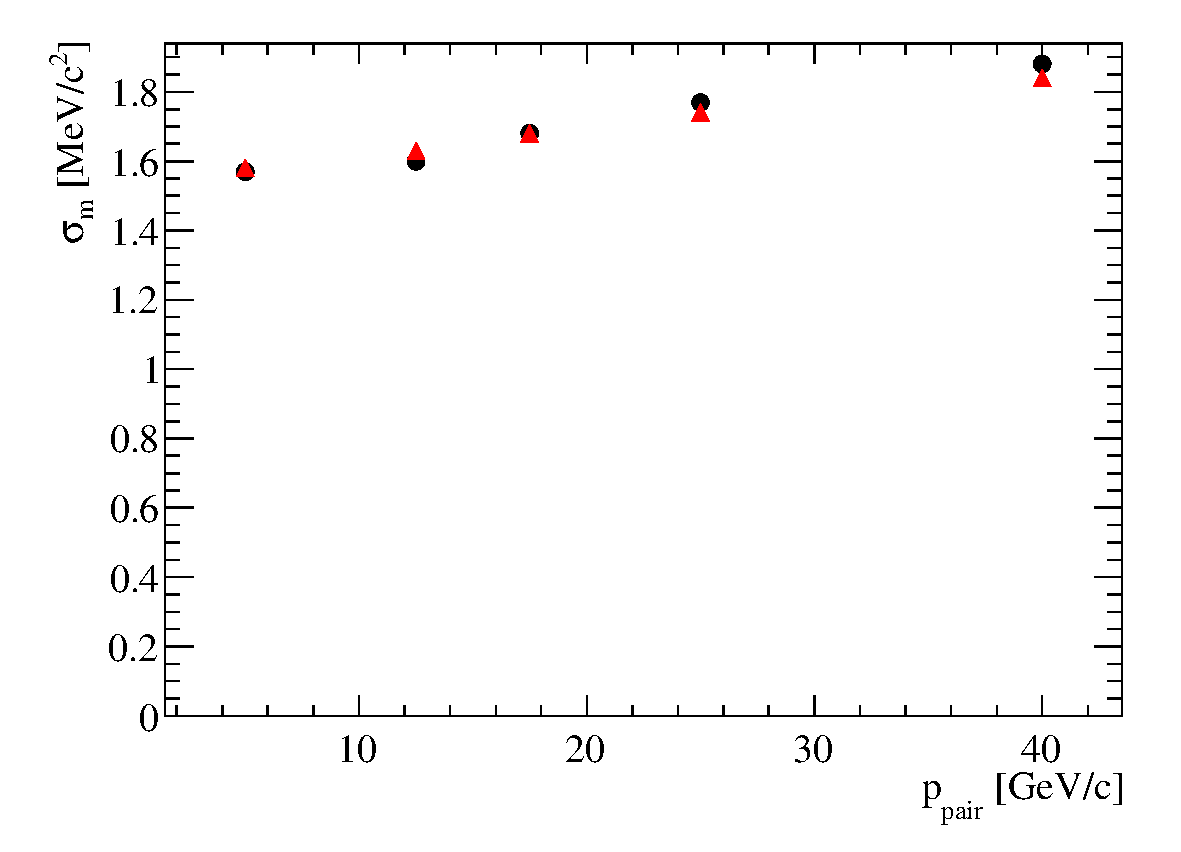
\includegraphics{figs/sigma_ppair.pdf}}
\caption{\small Mass resolution for the $\chicone \rightarrow J/\psi
  \mu^+ \mu^-$ decay sample versus $p_{pair}$. The black points are
  the results obtained with the full simulation, The red triangles are the results
  obtained with the emulator.  }
\label{fig:sigmappair}
\end{center}
\end{figure}
%
\begin{figure}[htb!]
\begin{center}
\resizebox{3.8in}{!}{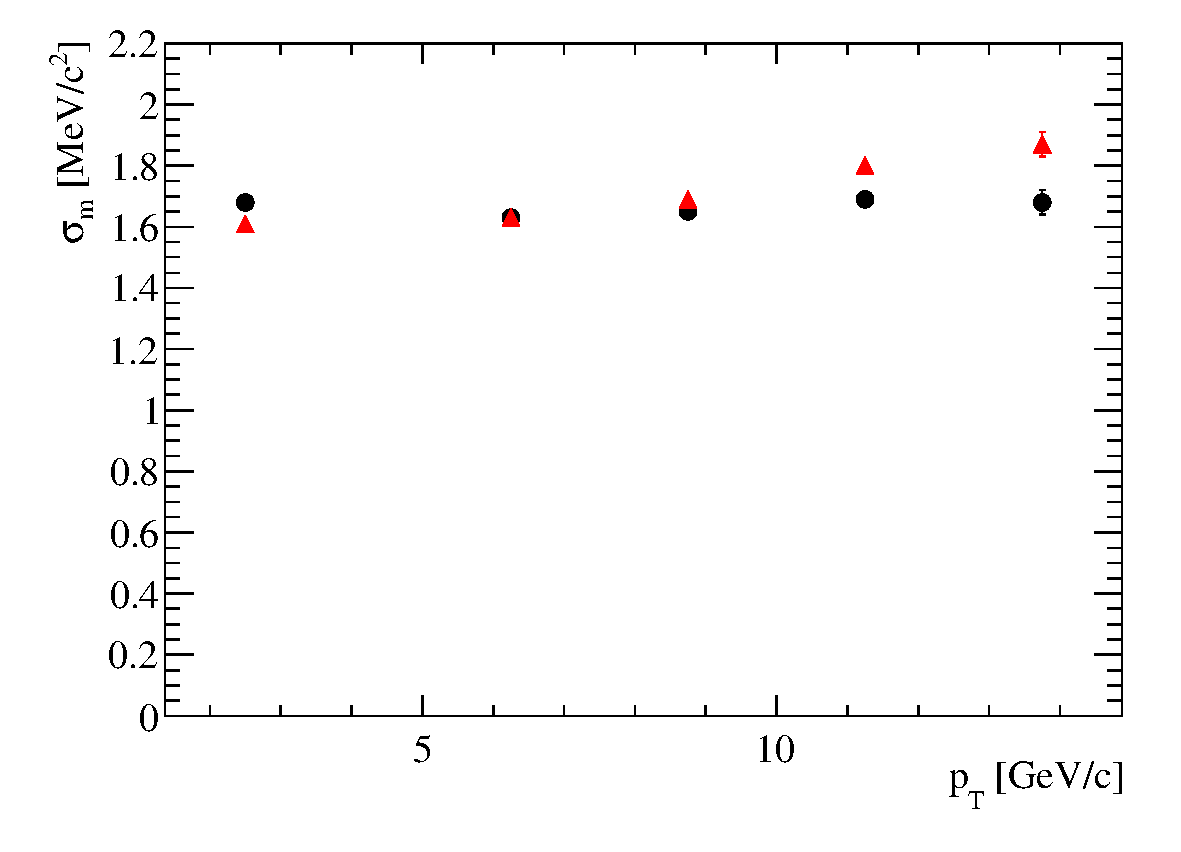
\includegraphics{figs/sigma_pt.pdf}}
\caption{\small Mass resolution for the $\chicone \rightarrow J/\psi
  \mu^+ \mu^-$ decay sample versus $\pt$.  The black points are
  the results obtained with the full simulation, The red triangles are the results
  obtained with the emulator. }
\label{fig:sigmapt}
\end{center}
\end{figure}
%
\begin{figure}[htb!]
\begin{center}
\resizebox{3.8in}{!}{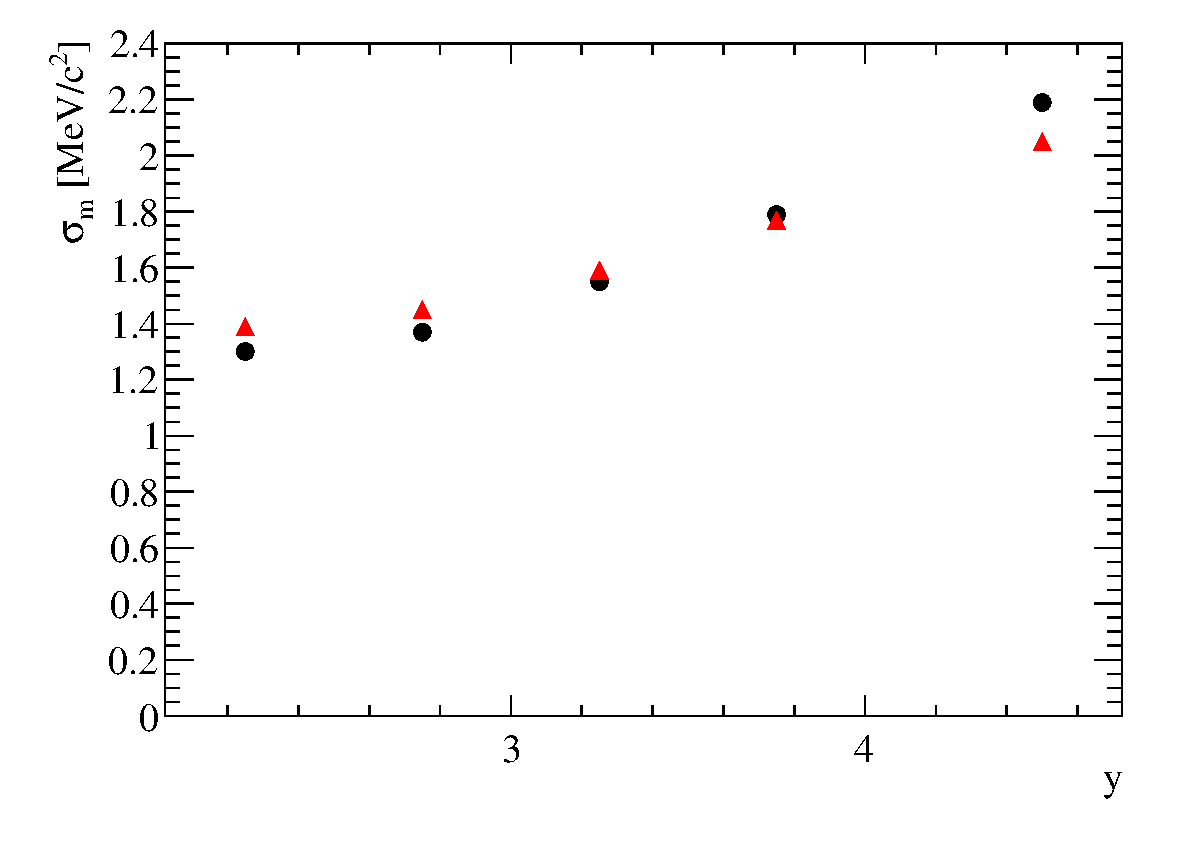
\includegraphics{figs/sigma_y.pdf}}
\caption{\small Mass resolution for the $\chicone \rightarrow J/\psi
  \mu^+ \mu^-$ decay sample versus $y$.  The black points are
  the results obtained with the full simulation, The red triangles are the results
  obtained with the emulator. }
\label{fig:sigmay}
\end{center}
\end{figure}

The second check is to compare the emulator and full simulation for
the modes $\psi(2S) \rightarrow J/\psi \pi^+ \pi^-$ and $X(3872)
\rightarrow J/\psi \pi^+ \pi^-$. The results are summarized in Table
\ref{tab:valid} and again indicate that the emulator reproduces the full
simulation at the level of $3 \%$ or better \footnote{The $\psi(2S)$
  sample is even at a different centre-of-mass energy making it a harsh test.}.

\begin{table}[htb!]
\caption{\small Comparison of the resolution found in the full
  simulation and with the emulator described in the text for several
  decay modes. }
\begin{center}
\small
\begin{tabular}{l|c|c|c|c}
Mode & Full MC Conditions & $\sigma^{fit}_m$ [$\mevcc$] &
                                                          $\sigma^{em}_m$
                                                          [$\mevcc$] &
  Ratio\\ \hline
$\chicone \rightarrow J/\psi \mu^+ \mu^-$  & 2016 & $1.66 \pm 0.01$ &
                                                                      $1.66
                                                                      \pm
                                                                      0.01$
                                                                     &
  1.0\\
$\chictwo \rightarrow J/\psi \mu^+ \mu^-$  & 2016 & $1.81 \pm 0.01$ &
                                                                      $1.83
                                                                      \pm
                                                                      0.01$
                                                                     &
  1.01\\
$\psi(2S) \rightarrow J/\psi \pi^+ \pi^-$  & 2011+12 & $2.13 \pm 0.01$
                                                        &  $2.10 \pm
                                                          0.01$ & 0.99
  \\
$X(3872) \rightarrow J/\psi \pi^+ \pi^-$  & 2016 &$2.62 \pm 0.01$ &
                                                                    $2.69
                                                                    \pm
                                                                    0.01$
                                                                     &
  1.03\\
\end{tabular}
\end{center}
\label{tab:valid}
\end{table} 



\begin{table}[htb!]
\caption{\small Comparison of the resolution found in the full
  simulation and with the emulator described in the text for several
  decay modes requring. The candidate is required to have $\pt > 10 \gevc$. }
\begin{center}
\small
\begin{tabular}{l|c|c|c|c}
Mode & Full MC Conditions & $\sigma^{fit}_m$ [$\mevcc$] &
                                                          $\sigma^{em}_m$
                                                          [$\mevcc$] &
  Ratio\\ \hline
$\chicone \rightarrow J/\psi \mu^+ \mu^-$  & 2016 & $1.70 \pm 0.02$ &
                                                                      $1.84
                                                                      \pm
                                                                      0.02$
                                                                     &
  1.08\\
$\chictwo \rightarrow J/\psi \mu^+ \mu^-$  & 2016 & $1.93 \pm 0.05$ &
                                                                      $2.13
                                                                      \pm
                                                                      0.05$
                                                                     &
  1.1\\
$\psi(2S) \rightarrow J/\psi \pi^+ \pi^-$  & 2011+12 & $2.26 \pm 0.03$
                                                        &  $2.38 \pm
                                                          0.03$ & 1.05
  \\
$X(3872) \rightarrow J/\psi \pi^+ \pi^-$  & 2016 &$2.75 \pm 0.02$ &
                                                                    $2.99
                                                                    \pm
                                                                    0.02$
                                                                     &
  1.08\\
\end{tabular}
\end{center}
\label{tab:valid10}
\end{table} 


\section{Data tuning}
\label{sec:data}
%
The emulator has been tuned to reproduce the full simulation. For the
$\chicone \rightarrow \jpsi \mu^+ \mu^-$ decay mode it is known that 
data and simulation agree within better than $10 \%$. 

 It is also known that the momentum resolution
in data is worse than simulation. This mainly effects the mass resolution for
modes with high energy release and is not very relevant for modes such
as $\chicone \rightarrow \jpsi \mu^+ \mu^-$. However, for completeness the
possibility to apply additional momentum smearing, derived from
comparisions between data and simulation using Run 2 data for the $B^+
\rightarrow J/\psi K^+$ data has been added to the emulator. Applying
it to the $\chicone \rightarrow \jpsi \mu^+ \mu^-$ decay mode it does not change
the mass resolution given by the emulator significantly.

\section{Conclusion}
\label{sec:conclusion}
%
In this note an emulator to estimate the mass resolution for the decay
$\chicone \rightarrow J/\psi \mu^+ \mu^-$ has been developed. The
emulator reproduces the resolution in the full simulation
 for this mode. Dividing data into regions of phase space
the agreement with the full simulation is generally found at the level
of a $5 \%$ or better . The worse level of agreement is at the $10 \%$ level
at high candidate $\pt$.  Tte model is flexible enough to
be used for similar topology modes where it reproduces the overall
resolution at the level of $3 \%$ or better. It is intended to use
this mode for studies of $\chi_b$ Dalitz decays. Though the work
desecribed here is adequate for that use-case various improvements
could be envisaged. First, more care could be taken in data-sample
selection to give a more uniform coverage of the phase space. Second,
the hyperparameters of the BDT have not been optimized beyond the
defaults suggested in TMVA. Finally, it would be better to train one
BDT rather than three which also takes into account the correlations
between the parameters. That would be possible in a framework such as
Tensorflow.

The regression model for the momentum resolution has wider
applicability and could be used directly in \textbf{RapidSim} or other
fast simulation packages. An insight gained from this study is the
importance of the resolution on the track slopes for modes with soft
tracks. This is greatly improved by application of a pointing constraint
to the PV in the decay tree fit.  This needs to considered when using
a fast simulation. To properly account for this requires either to
explicitly apply this constraint or to properly parameterize the
effect for different topologies.



\clearpage

\appendix

% Do not include this in any draft (just for information in the template)
%\section{Acknowledgements paragraph}

Include the following text in the Acknowledgements section in all paper
drafts. It is not needed for analysis notes or conference reports.

The text below are the acknowledgements as approved by the collaboration
board. Extending the acknowledgements to include individuals from outside the
collaboration who have contributed to the analysis should be approved by the
EB. The extra acknowledgements are normally placed before the standard 
acknowledgements, unless it matches better with the text of the standard 
acknowledgements to put them elsewhere. They should be included in the draft 
for the first circulation. Except in exceptional circumstances, to be approved by the
EB chair, authors of the paper should not be named in extended acknowledgements.

%\vspace{1cm}

\section*{Acknowledgements}
%
% These Acknowledgements valid from 14-Aug-2018
%
\noindent We express our gratitude to our colleagues in the CERN
accelerator departments for the excellent performance of the LHC. We
thank the technical and administrative staff at the LHCb
institutes.
We acknowledge support from CERN and from the national agencies:
CAPES, CNPq, FAPERJ and FINEP (Brazil); 
MOST and NSFC (China); 
CNRS/IN2P3 (France); 
BMBF, DFG and MPG (Germany); 
INFN (Italy); 
NWO (Netherlands); 
MNiSW and NCN (Poland); 
MEN/IFA (Romania); 
MSHE (Russia); 
MinECo (Spain); 
SNSF and SER (Switzerland); 
NASU (Ukraine); 
STFC (United Kingdom); 
NSF (USA).
We acknowledge the computing resources that are provided by CERN, IN2P3
(France), KIT and DESY (Germany), INFN (Italy), SURF (Netherlands),
PIC (Spain), GridPP (United Kingdom), RRCKI and Yandex
LLC (Russia), CSCS (Switzerland), IFIN-HH (Romania), CBPF (Brazil),
PL-GRID (Poland) and OSC (USA).
We are indebted to the communities behind the multiple open-source
software packages on which we depend.
Individual groups or members have received support from
AvH Foundation (Germany);
EPLANET, Marie Sk\l{}odowska-Curie Actions and ERC (European Union);
ANR, Labex P2IO and OCEVU, and R\'{e}gion Auvergne-Rh\^{o}ne-Alpes (France);
Key Research Program of Frontier Sciences of CAS, CAS PIFI, and the Thousand Talents Program (China);
RFBR, RSF and Yandex LLC (Russia);
GVA, XuntaGal and GENCAT (Spain);
the Royal Society
and the Leverhulme Trust (United Kingdom);
Laboratory Directed Research and Development program of LANL (USA).


% Comment this in for paper drafts; do not include this in analysis note and conference reports
%\section*{Acknowledgements}
%
% These Acknowledgements valid from 14-Aug-2018
%
\noindent We express our gratitude to our colleagues in the CERN
accelerator departments for the excellent performance of the LHC. We
thank the technical and administrative staff at the LHCb
institutes.
We acknowledge support from CERN and from the national agencies:
CAPES, CNPq, FAPERJ and FINEP (Brazil); 
MOST and NSFC (China); 
CNRS/IN2P3 (France); 
BMBF, DFG and MPG (Germany); 
INFN (Italy); 
NWO (Netherlands); 
MNiSW and NCN (Poland); 
MEN/IFA (Romania); 
MSHE (Russia); 
MinECo (Spain); 
SNSF and SER (Switzerland); 
NASU (Ukraine); 
STFC (United Kingdom); 
NSF (USA).
We acknowledge the computing resources that are provided by CERN, IN2P3
(France), KIT and DESY (Germany), INFN (Italy), SURF (Netherlands),
PIC (Spain), GridPP (United Kingdom), RRCKI and Yandex
LLC (Russia), CSCS (Switzerland), IFIN-HH (Romania), CBPF (Brazil),
PL-GRID (Poland) and OSC (USA).
We are indebted to the communities behind the multiple open-source
software packages on which we depend.
Individual groups or members have received support from
AvH Foundation (Germany);
EPLANET, Marie Sk\l{}odowska-Curie Actions and ERC (European Union);
ANR, Labex P2IO and OCEVU, and R\'{e}gion Auvergne-Rh\^{o}ne-Alpes (France);
Key Research Program of Frontier Sciences of CAS, CAS PIFI, and the Thousand Talents Program (China);
RFBR, RSF and Yandex LLC (Russia);
GVA, XuntaGal and GENCAT (Spain);
the Royal Society
and the Leverhulme Trust (United Kingdom);
Laboratory Directed Research and Development program of LANL (USA).


\section{Comparisions of fit and emulated uncertainties on the track slopes}
\label{sec:slopeplots}
%
\begin{figure}[h!]
\centering
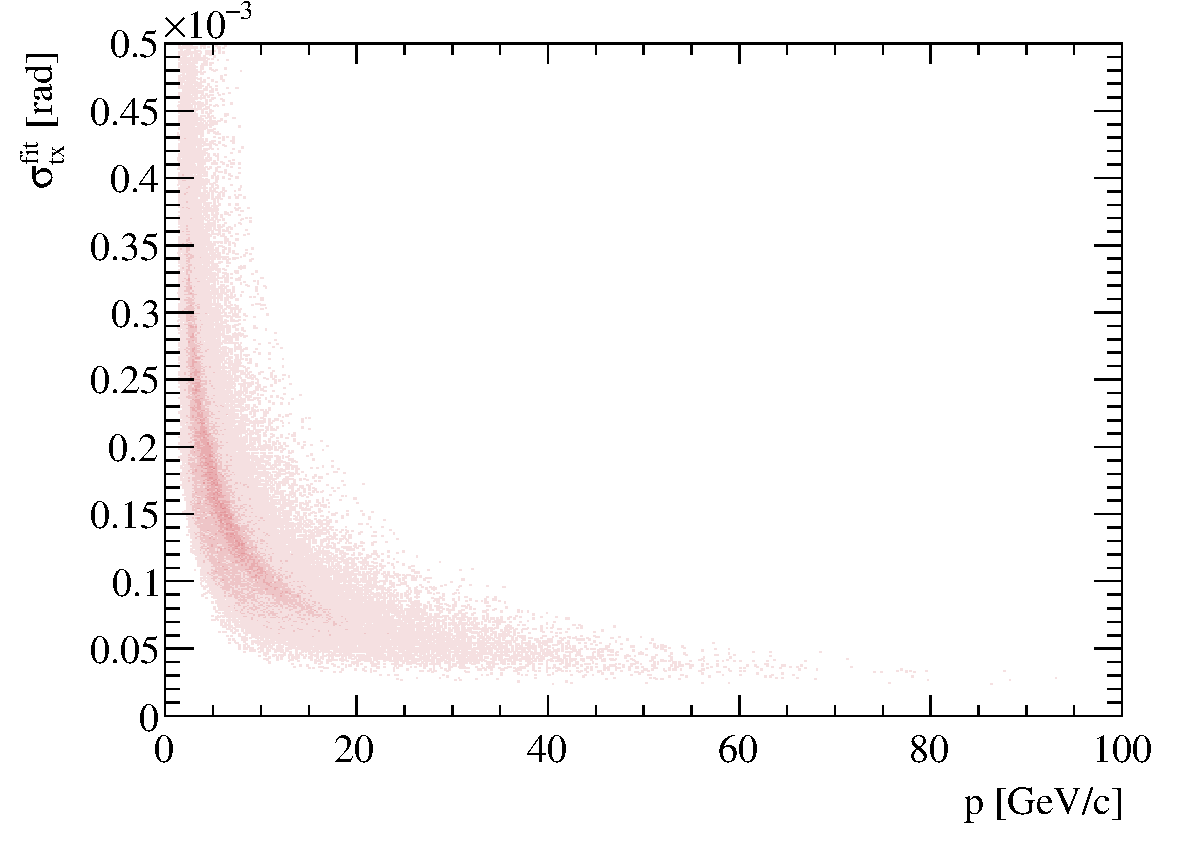
\includegraphics[width=0.48\textwidth]{figs/etx-fit.pdf}
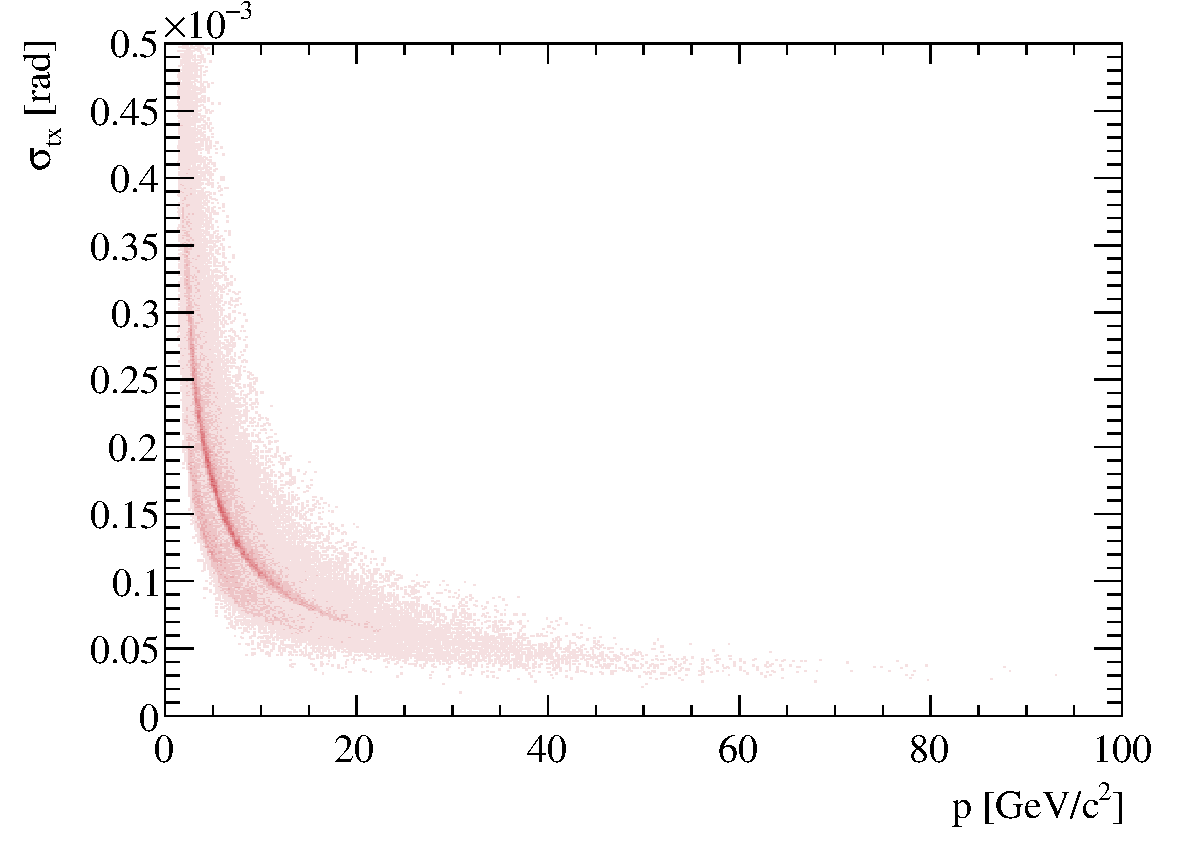
\includegraphics[width=0.48\textwidth]{figs/etx-em.pdf}
\caption{(Left) $\sigma^{fit}_{tx}$ versus $p$. (Right)
  $\sigma^{em}_{tx}$ versus $p$.}
\label{fig:emtxp}
\end{figure}
%
\begin{figure}[h!]
\centering
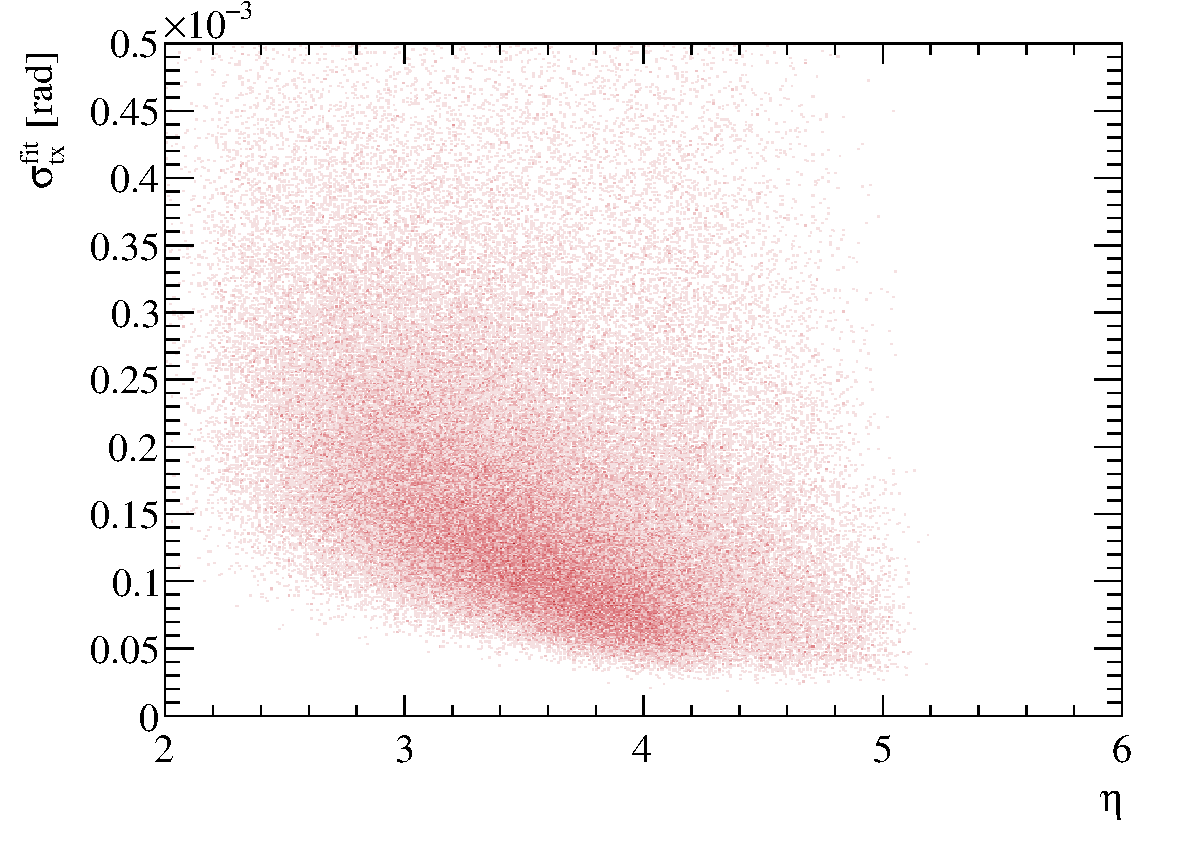
\includegraphics[width=0.48\textwidth]{figs/etx-eta-fit.pdf}
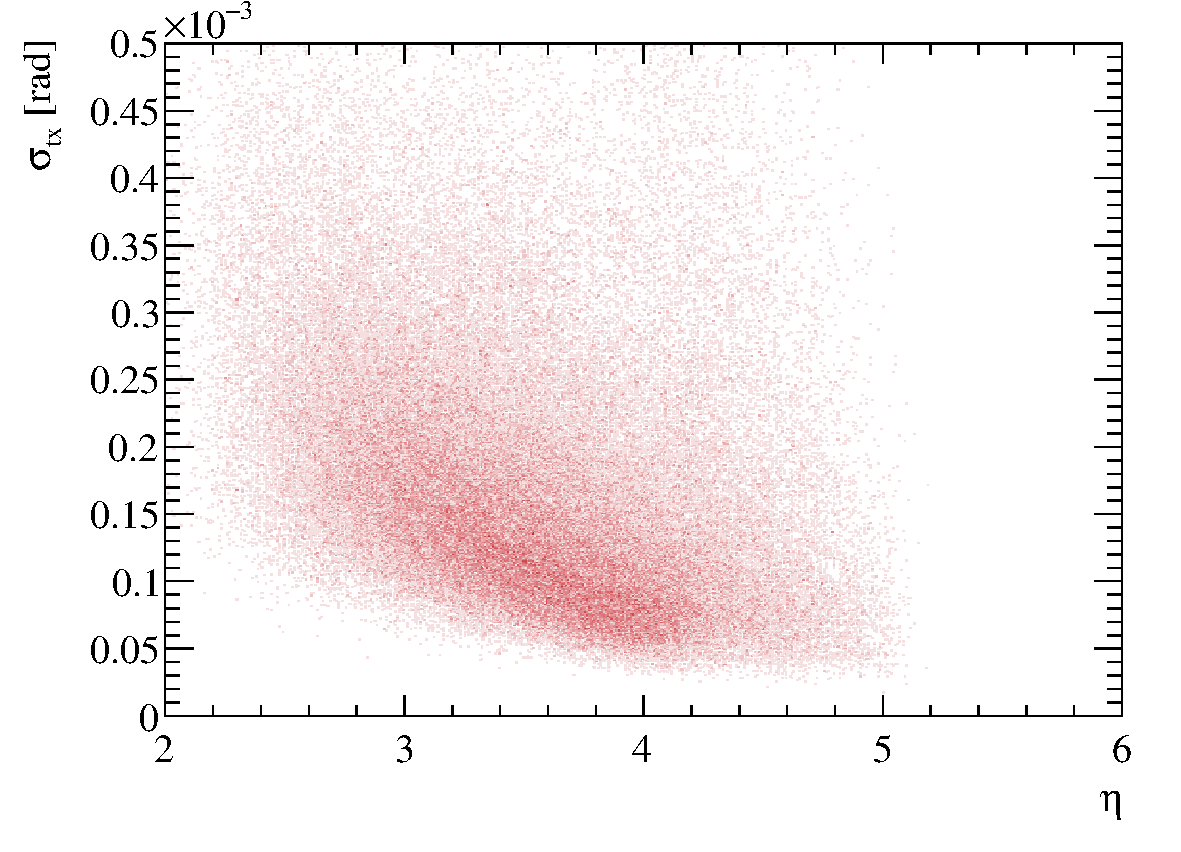
\includegraphics[width=0.48\textwidth]{figs/etx-eta-em.pdf}
\caption{(Left) $\sigma^{fit}_{tx}$ versus $\eta$. (Right)
  $\sigma^{em}_{tx}$ versus $\eta$.}
\label{fig:emtxeta}
\end{figure}
%
\begin{figure}[h!]
\centering
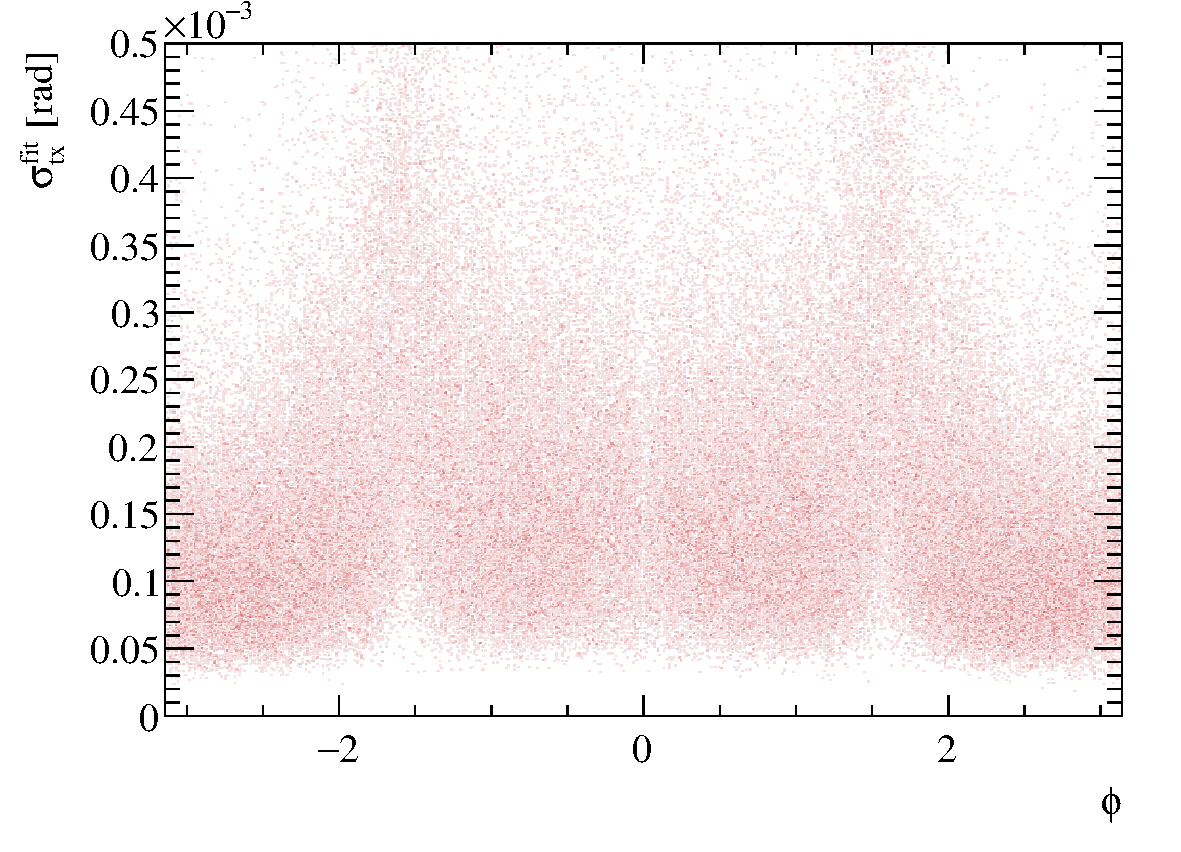
\includegraphics[width=0.48\textwidth]{figs/etx-phi-fit.pdf}
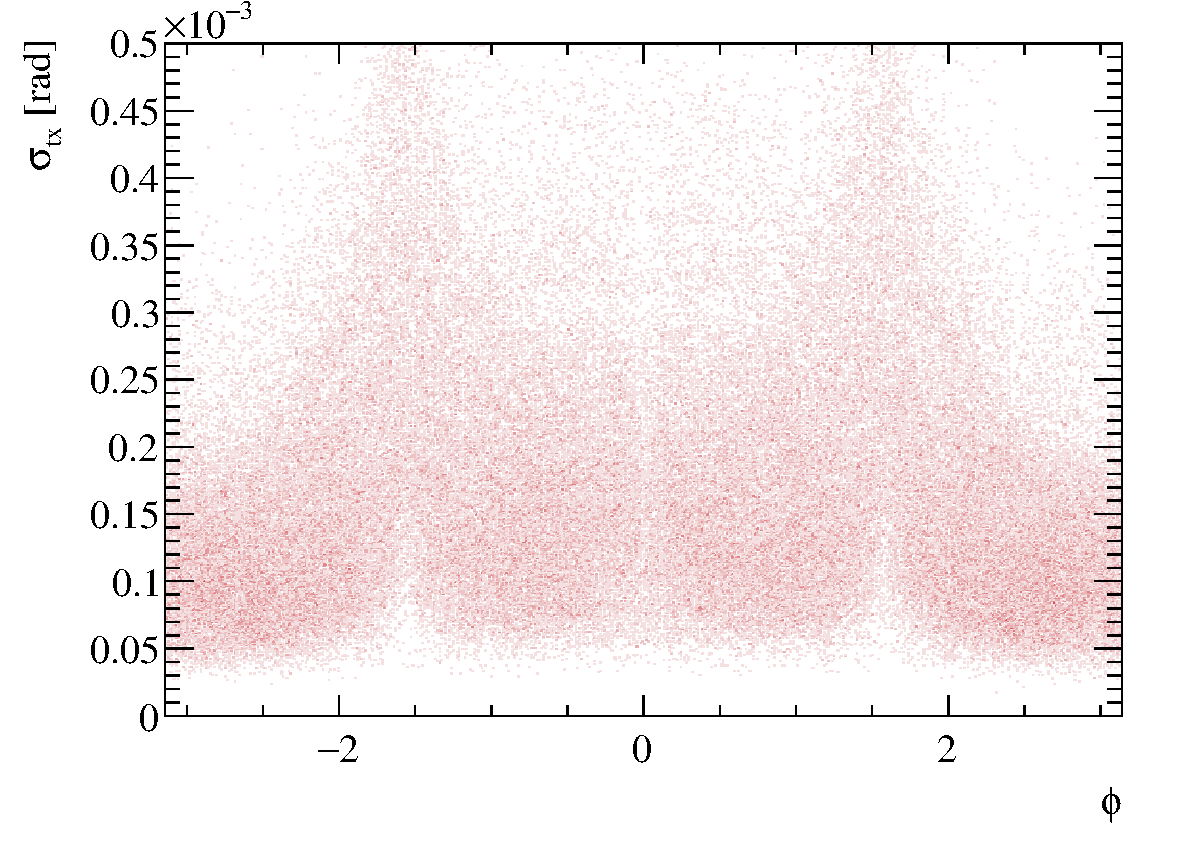
\includegraphics[width=0.48\textwidth]{figs/etx-phi-em.pdf}
\caption{(Left) $\sigma^{fit}_{tx}$ versus $\phi$. (Right)
  $\sigma^{em}_{tx}$ versus $\phi$.}
\label{fig:emtxphi}
\end{figure}
%

%
\begin{figure}[h!]
\centering
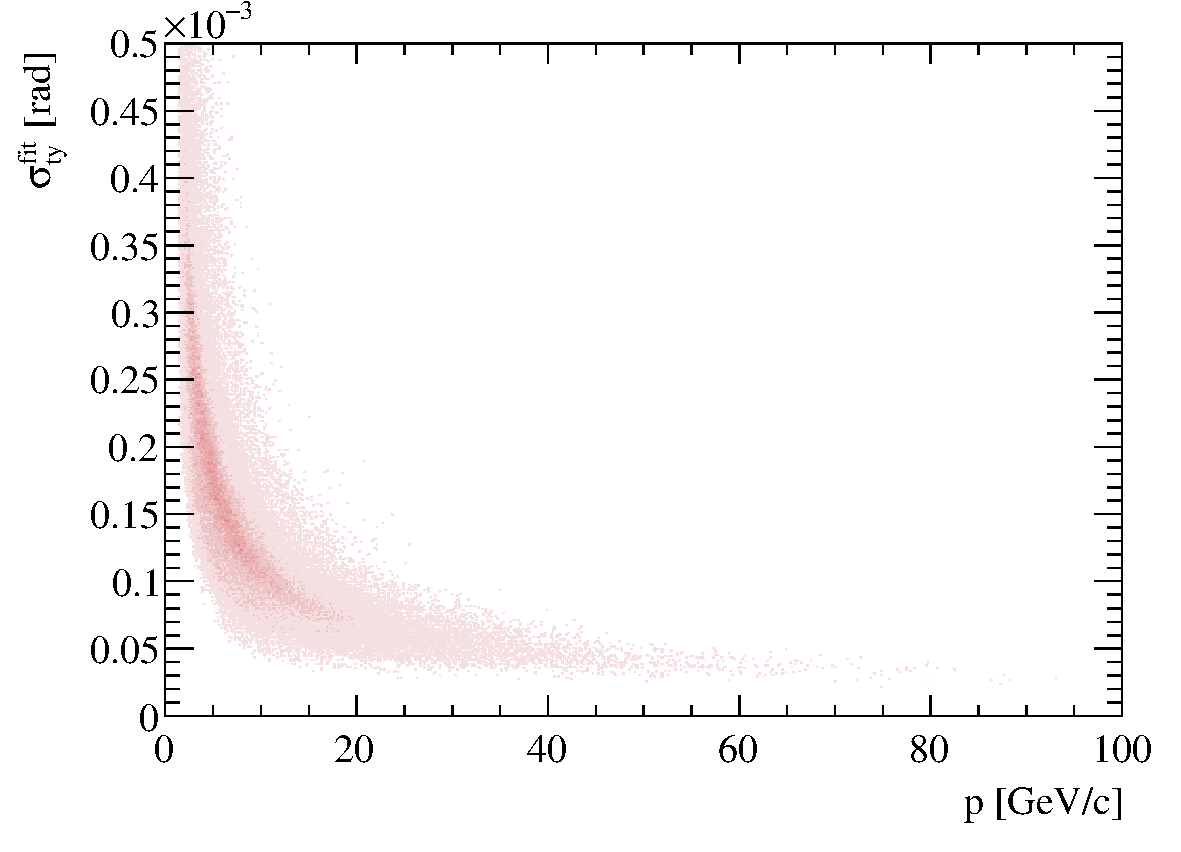
\includegraphics[width=0.48\textwidth]{figs/ety-fit.pdf}
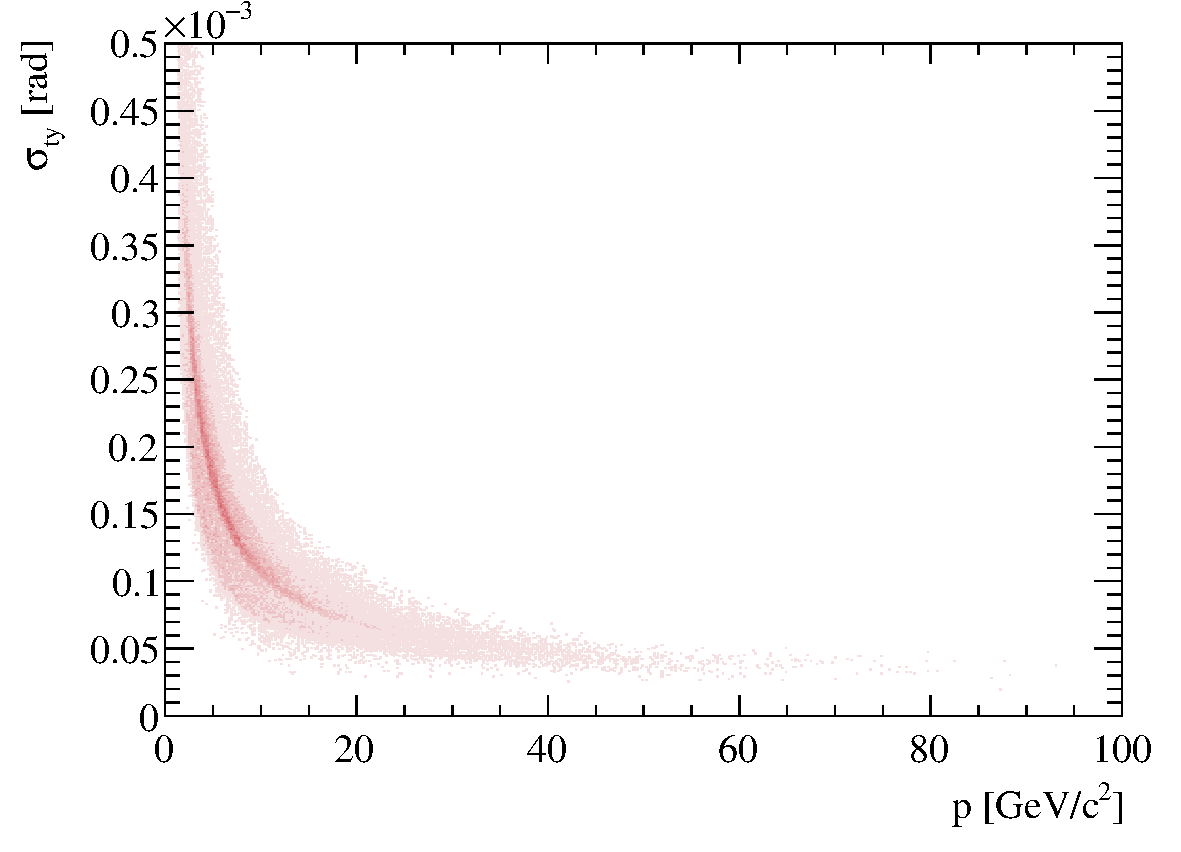
\includegraphics[width=0.48\textwidth]{figs/ety-em.pdf}
\caption{(Left) $\sigma^{fit}_{ty}$ versus $p$. (Right)
  $\sigma^{em}_{ty}$ versus $p$.}
\label{fig:emtyp}
\end{figure}
%
%
\begin{figure}[h!]
\centering
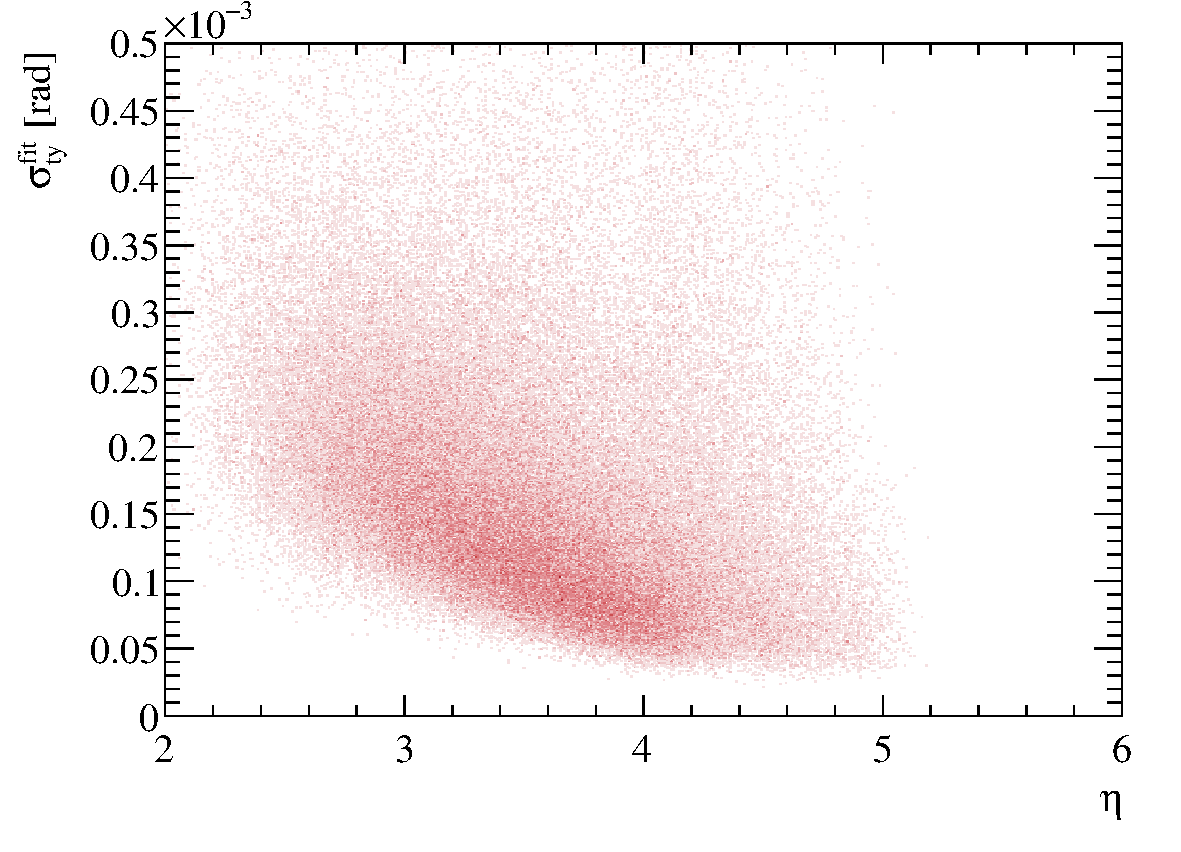
\includegraphics[width=0.48\textwidth]{figs/ety-eta-fit.pdf}
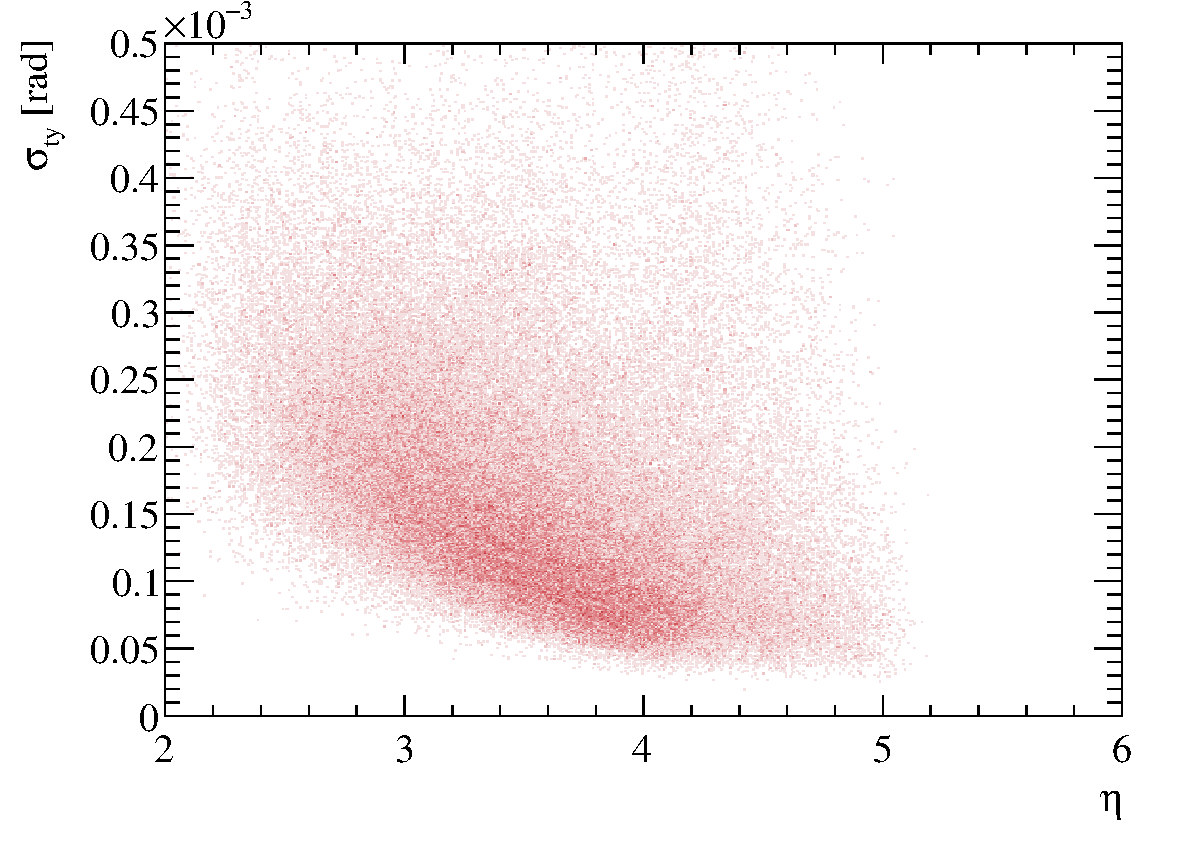
\includegraphics[width=0.48\textwidth]{figs/ety-eta-em.pdf}
\caption{(Left) $\sigma^{fit}_{ty}$ versus $\eta$. (Right)
  $\sigma^{em}_{ty}$ versus $\eta$.}
\label{fig:emtyeta}
\end{figure}
%
%
\begin{figure}[h!]
\centering
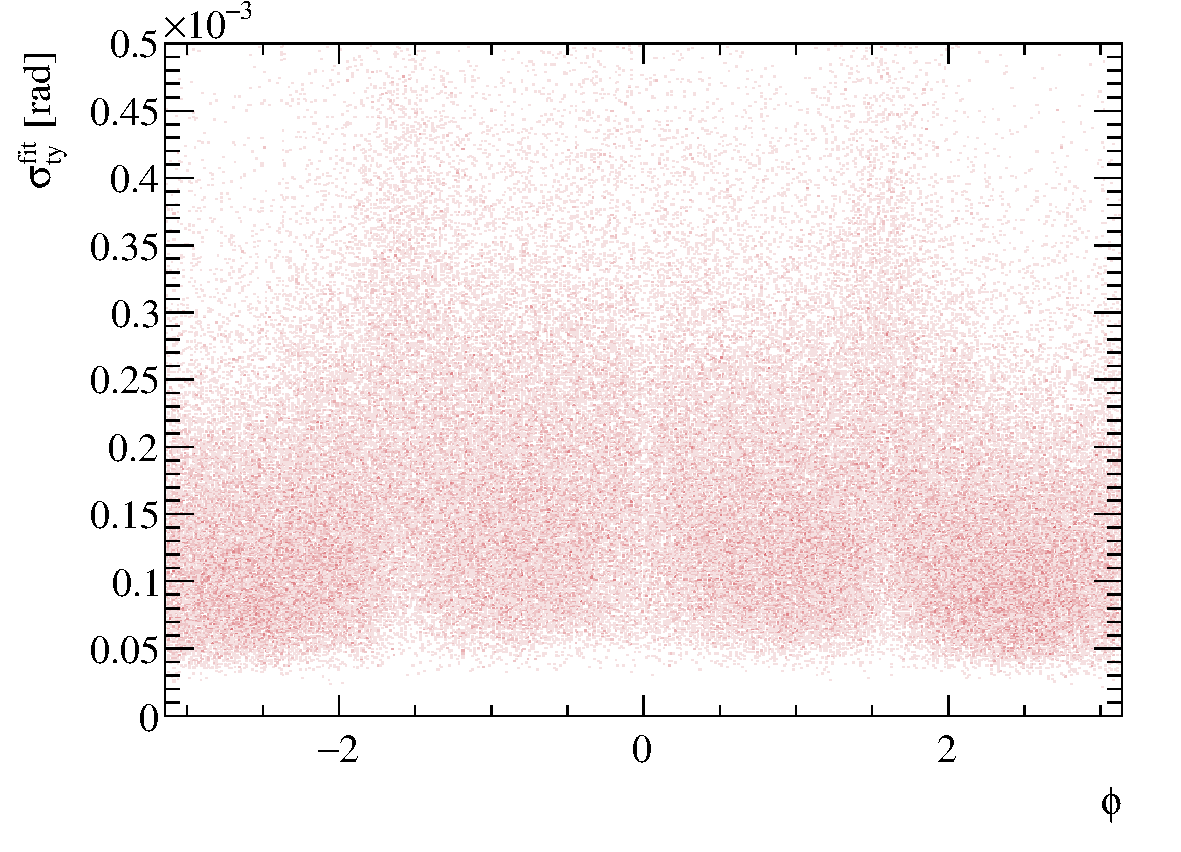
\includegraphics[width=0.48\textwidth]{figs/ety-phi-fit.pdf}
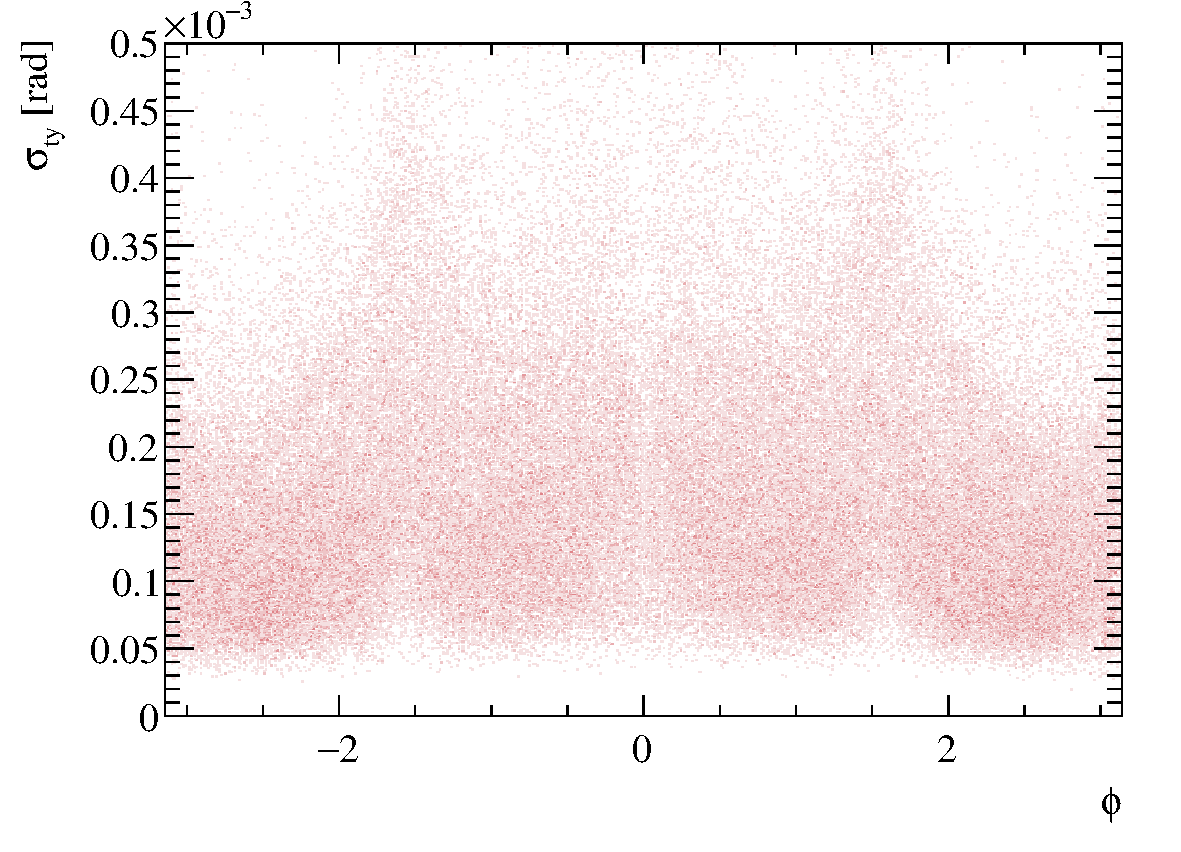
\includegraphics[width=0.48\textwidth]{figs/ety-phi-em.pdf}
\caption{(Left) $\sigma^{fit}_{ty}$ versus $\phi$. (Right)
  $\sigma^{em}_{ty}$ versus $\phi$.}
\label{fig:emtyphi}
\end{figure}
%


\clearpage

\section{Track slopes: Parametric approach}
\label{sec:slopes}
%
An alternative parametric approach was also developed to model the slopes. A gaussian
fit is made to the difference between the true and reconstructed
slopes in bins of momentum. A  fit of the form
\begin{equation}
\sigma(tx) = \sqrt{A_{res}^2 + \frac{B_{ms}^2}{p^2}}
\label{eq:sloperes}
\end{equation}
 is then made to the resulting distributions of the slopes in $x$ and
 $y$ versus momentum. As example this is shown for the $y$ slopes in  Fig. \ref{fig:sloperes}. In this form the first term accounts for
the effect of detector resolution and the second for multiple
scattering. The fit, shown in Fig. \ref{fig:slopefitty},  gives $A_{res} = 7 \times 10^{-5}$ and $B_{ms} =
0.9 \mevc$. This method is simple if not perfect, in particular the quality of
the Gaussian slice fits at low $p$ is poor ($\chi^2/ndof
\sim 6$). This reflects the importance of of other variables and also
the the non-Gaussian tails in the multiple scattering distribution. 
\begin{figure}[htb!]
\begin{center}
\resizebox{3.8in}{!}{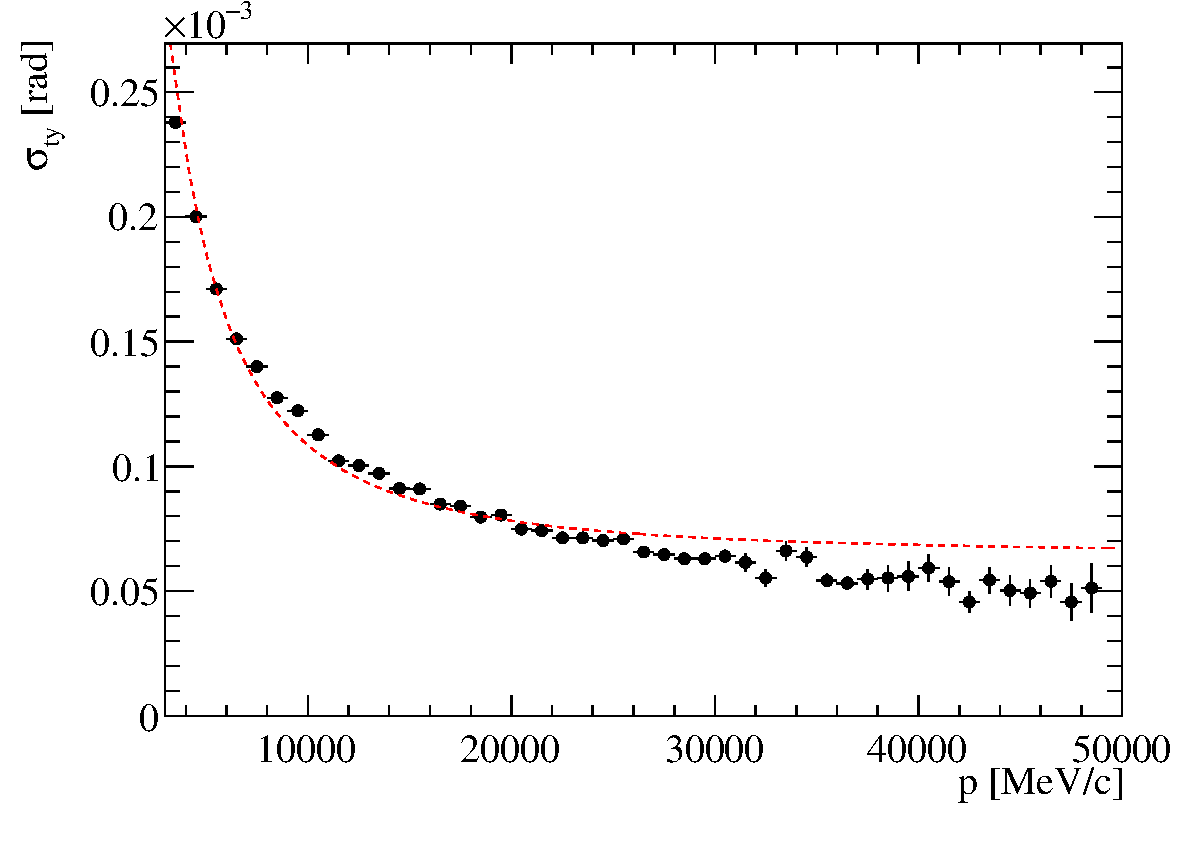
\includegraphics{figs/slopefit-ty.pdf}}
\caption{\small Track slope resolution in y versus momentum. A fit to the
  form given in Eq. \ref{eq:sloperes} is superimposed.}
\label{fig:slopefitty}
\end{center}
\end{figure}
%

As in the case of the track momentum uncertainty the pulls from this
approach are not one. The Gaussian core, which encompasses $84 \%$ of
the distribution,  has a width of 0.8  and the tail as width of 1.8.  

Other more complicated parameterizations two-dimensional binning and fitting schemes ($e.g.$ in $\pt$ and
$\eta$ bins ) were tried but found not
to improve the results significantly (whilst adding
complexity). Table~\ref{tab:valids} shows the comparision of the mass resolution
found using this approach and the full simulation for the decay modes
considered. The agreement compared to the MVA approach (Table \ref{tab:valid}) is
noticeably worse.  Hence, since this method gives worse results and is
more involved it was not considered further.

\begin{table}[htb!]
\caption{\small Comparison of the resolution found in the full
  simulation and with the emulator described in the text for several
  decay modes. }
\begin{center}
\small
\begin{tabular}{l|c|c|c|c}
Mode & Full MC Conditions & $\sigma^{fit}_m$ [$\mevcc$] &
                                                          $\sigma^{em}_m$
                                                          [$\mevcc$] &
  Ratio\\ \hline
$\chicone \rightarrow J/\psi \mu^+ \mu^-$  & 2016 & $1.66 \pm 0.01$ &
                                                                      $1.70
                                                                      \pm
                                                                      0.01$
                                                                     &
  1.02\\
$\chictwo \rightarrow J/\psi \mu^+ \mu^-$  & 2016 & $1.81 \pm 0.01$ &
                                                                      $1.87
                                                                      \pm
                                                                      0.01$
                                                                     &
  1.03\\
$\psi(2S) \rightarrow J/\psi \pi^+ \pi^-$  & 2011+12 & $2.13 \pm 0.01$
                                                        &  $2.18 \pm
                                                          0.01$ & 1.02
  \\
$X(3872) \rightarrow J/\psi \pi^+ \pi^-$  & 2016 &$2.62 \pm 0.01$ &
                                                                    $2.75
                                                                    \pm
                                                                    0.01$
                                                                     &
  1.05\\
\end{tabular}
\end{center}
\label{tab:valids}
\end{table} 


%% $Id: appendix.tex 124316 2018-10-30 11:59:39Z pkoppenb $
% ===============================================================================
% Purpose: appendix to the standard template: standard symbol alises from Ulrik
% Author: Tomasz Skwarnicki
% Created on: 2009-09-24
% ===============================================================================

%{\noindent\normalfont\bfseries\Large Appendices}
\section*{Appendices}

\appendix

\section{Standard References}
\label{sec:StandardReferences}
Below is a list of common references, as
well as a list of all \lhcb publications. 
As they are already in prepared bib files, they can be used as simply as
\texttt{\textbackslash cite\{Alves:2008zz\}} to get the \lhcb detector paper. 
The references are defined in the files \texttt{main.bib},  \texttt{LHCb-PAPER.bib},
\texttt{LHCb-CONF.bib}, \texttt{LHCb-DP.bib} \texttt{LHCb-TDR.bib} files, with obvious contents.
Each of these have their \texttt{LHCb-ZZZ-20XX-0YY} number as their cite code.
If you believe there is a problem with the formatting or
content of one of the entries, then get in contact with the Editorial
Board rather than just editing it in your local file,
since you are likely to need the latest version just before submitting the article.

%%%%%%%%%%%%%%%%%%%%%%%%%%%%%%%%%%
\newcommand{\showcite}[1]{\texttt{#1}~\cite{#1}}%
\newcommand{\revshowcite}[1]{\begin{minipage}{1cm}\cite{#1}\end{minipage}\texttt{#1}}%
%%%%%%%%%%%%%%%%%%%%%%%%%%%%%%%%%%
\begin{center}
  \begin{longtable}{ll}
\caption{\small Standard references.}\label{tab:Refs}
\endfirsthead
\multicolumn{2}{c}{ -- continued from previous page.}
\endhead
\endfoot
\endlastfoot
\hline
Description & \begin{minipage}{1cm}Ref.\end{minipage}\texttt{cite} code \\
\hline % physics resources
PDG 2018 & \revshowcite{PDG2018} \\
PDG 2016 & \revshowcite{PDG2016}  \\ % {PDG2016} \\
PDG 2014 & \revshowcite{PDG2014}  \\ % {PDG2014} \\
HFlav 2016 & \revshowcite{HFLAV16}  \\ % {HFLAV16} \\
HFlav (pre-2016)  & \revshowcite{Amhis:2014hma}  \\ % {Amhis:2014hma} \\
CKMfitter group & \revshowcite{CKMfitter2005}  \\ % {CKMfitter2005} \\
CKMfitter group & \revshowcite{CKMfitter2015}  \\ % {CKMfitter2015} \\
UTfit (Standard Model/CKM) & \revshowcite{UTfit-UT}  \\ % {UTfit-UT} \\
UTfit (New Physics) & \revshowcite{UTfit-NP}  \\ % {UTfit-NP} \\
\hline % simulation, LHCb
\lhcb simulation & \revshowcite{LHCb-PROC-2011-006}  \\ % {LHCb-PROC-2011-006} \\
\pythia & \revshowcite{Sjostrand:2006za, *Sjostrand:2007gs}  \\ % {Sjostrand:2006za, *Sjostrand:2007gs} \\
\lhcb \pythia tuning & \revshowcite{LHCb-PROC-2010-056}  \\ % {LHCb-PROC-2010-056} \\
\geant & \revshowcite{Allison:2006ve, *Agostinelli:2002hh}  \\ % {Allison:2006ve, *Agostinelli:2002hh} \\
\evtgen & \revshowcite{Lange:2001uf}   \\ % {Lange:2001uf} \\
\photos & \revshowcite{Golonka:2005pn}   \\ % {Golonka:2005pn} \\
RapidSim & \revshowcite{Cowan:2016tnm}  \\ % {Cowan:2016tnm} \\
\dirac & \revshowcite{Tsaregorodtsev:2010zz,*BelleDIRAC}  \\ % {Tsaregorodtsev:2010zz, *BelleDIRAC}  \\
SMOG & \revshowcite{FerroLuzzi:2005em}  \\ % {FerroLuzzi:2005em} \\
HLT2 topo & \revshowcite{BBDT}  \\ % {BBDT} \\
PIDCalib (for Run~1) & \revshowcite{LHCb-PUB-2016-021}  \\ % {LHCb-PUB-2016-021} \\
Ghost probability & \revshowcite{DeCian:2255039}  \\ % {DeCian:2255039}\\
DecayTreeFitter & \revshowcite{Hulsbergen:2005pu}  \\ % {Hulsbergen:2005pu} \\
\sPlot & \revshowcite{Pivk:2004ty}  \\ % {Pivk:2004ty} \\
sFit & \revshowcite{Xie:2009rka}  \\ % {Xie:2009rka} \\
Punzi's optimization & \revshowcite{Punzi:2003bu}  \\ % {Punzi:2003bu} \\
\hline % selection
BDT & \revshowcite{Breiman}  \\ % {Breiman} \\
BDT training & \revshowcite{AdaBoost}  \\ % {AdaBoost} \\
TMVA\footnote{Do not cite this instead of the actual reference for the MVA being used.}  & \revshowcite{Hocker:2007ht,*TMVA4}  \\ % {Hocker:2007ht,*TMVA4} \\
RooUnfold & \revshowcite{Adye:2011gm}  \\ % {Adye:2011gm} \\
Scikit & \revshowcite{Scikit}  \\ % {Scikit} \\
\textsc{Laura}$^{++}$ & \revshowcite{Back:2017zqt}  \\ % {Back:2017zqt} \\
\texttt{hep-ml} & \revshowcite{Rogozhnikov:2016bdp}  \\ % {Rogozhnikov:2016bdp} \\
\hline % Fits
Crystal Ball function\footnote{A valid alternative for most papers where the normalisation is not critical is to use the expression``Gaussian function with a low-mass power-law tail'' or ``Gaussian function with power-law tails''. In that case, no citation is needed} & \revshowcite{Skwarnicki:1986xj}  \\ % {Skwarnicki:1986xj} \\
Hypatia & \revshowcite{Santos:2013gra}  \\ % {Santos:2013gra}\\
Wilks' theorem & \revshowcite{Wilks:1938dza}  \\ % {Wilks:1938dza}\\
CL$_s$ method & \revshowcite{CLs}  \\ % {CLs} \\
Bootstrapping & \revshowcite{efron:1979}  \\ % {efron:1979} \\
Blatt--Weisskopf barrier & \revshowcite{Blatt:1952ije}  \\ % {Blatt:1952ije} \\
\hline % LHC
$f_s/f_d$ & \revshowcite{fsfd}  \\ % {fsfd} \\
LHC beam energy uncertainty  & \revshowcite{PhysRevAccelBeams.20.081003}  \\ % {PhysRevAccelBeams.20.081003}\\
EW Baryogenesis \& \CP &  \revshowcite{Huet:1994jb}  \\ % {Huet:1994jb} \\
Baryon asymmetry \& SM \CP &  \revshowcite{Gavela:1994dt}  \\ % {Gavela:1994dt} \\
Baryon asymmetry \& SM \CP &  \revshowcite{Gavela:1993ts}  \\ % {Gavela:1993ts} \\
\hline % standard physics papers
Lee, Weinberg, Zumino & \revshowcite{Lee:1967iu}  \\ % {Weinberg:1967} \\
Cabibbo, Kobayashi, Maskawa & \revshowcite{Cabibbo:1963yz,*Kobayashi:1973fv}  \\ % {Cabibbo:1963yz,*Kobayashi:1973fv} \\
Gell-Mann, Zweig & \revshowcite{GellMann:1964nj,*Zweig:352337}  \\ % {GellMann:1964nj,*Zweig:352337} \\
\end{longtable}
%  \end{tabular}
\end{center}

\begin{center}
\begin{longtable}{ll}
\caption{\small LHCb detector performance papers.}\label{tab:LHCb-DPs}
\endfirsthead
\multicolumn{2}{c}{ -- continued from previous page.}
\endhead
\endfoot
\endlastfoot
\hline
    \hline
    \texttt{LHCb-DP} number & Title \\
    \hline
    \showcite{LHCb-DP-2018-004} & 
    {\small ReDecay}\\
    \showcite{LHCb-DP-2018-003} & 
    {\small Radiation damage in TT}\\
    \showcite{LHCb-DP-2018-002} & %{LHCb-DP-2018-002} &
    {\small VeLo material map using SMOG}\\
    \showcite{LHCb-DP-2018-001} & %{LHCb-DP-2018-001} &
    {\small PIDCalib for Run 2 (use Ref.~\cite{LHCb-PUB-2016-021} for Run~1)} \\
    \showcite{LHCb-DP-2017-001} & %{LHCb-DP-2017-001}&
    {\small Performance of the Outer Tracker --- Run 2}\\
    \showcite{LHCb-DP-2016-003} & %{LHCb-DP-2016-003} &
    {\small HeRSCheL} \\
    \showcite{LHCb-PROC-2015-018} & %{LHCb-PROC-2015-018} &
    {\small Topological trigger reoptimization --- Run 2} \\
    \showcite{LHCb-PROC-2015-011} & %{LHCb-PROC-2015-011} &
    {\small Turbo and real-time alignment --- Run 2} \\
    \showcite{LHCb-DP-2016-001} & %{LHCb-DP-2016-001} &
    {\small TESLA project --- Run 2} \\
    \showcite{LHCb-DP-2014-002} & %{LHCb-DP-2014-002} &
    {\small LHCb detector performance} \\
    \showcite{LHCb-DP-2014-001} & %{LHCb-DP-2014-001} &
    {\small Performance of the LHCb Vertex Locator} \\
    \showcite{LHCb-DP-2013-004} & %{LHCb-DP-2013-004} &
    {\small Performance of the LHCb calorimeters} \\
    \showcite{LHCb-DP-2013-003} & %{LHCb-DP-2013-003} &
    {\small Performance of the LHCb Outer Tracker} \\
    \showcite{LHCb-DP-2013-002} & %{LHCb-DP-2013-002} &
    {\small Measurement of the track reconstruction efficiency at LHCb} \\
    \showcite{LHCb-DP-2013-001} & %{LHCb-DP-2013-001} &
    {\small Performance of the muon identification at LHCb} \\
    \showcite{LHCb-DP-2012-005} & %{LHCb-DP-2012-005} &
    {\small Radiation damage in the LHCb Vertex Locator} \\
    \showcite{LHCb-DP-2012-004} & %{LHCb-DP-2012-004} &
    {\small The \lhcb trigger and its performance in 2011} \\
    \showcite{LHCb-DP-2012-003} & %{LHCb-DP-2012-003} &
    {\small Performance of the \lhcb RICH detector at the LHC} \\
    \showcite{LHCb-DP-2012-002} & %{LHCb-DP-2012-002} &
    {\small Performance of the LHCb muon system} \\
    \showcite{LHCb-DP-2012-001} & %{LHCb-DP-2012-001} &
    {\small Radiation hardness of the LHCb Outer Tracker} \\
    \showcite{LHCb-DP-2011-002} & %{LHCb-DP-2011-002} &
    {\small Simulation of machine induced background \dots} \\
    \showcite{LHCb-DP-2011-001} & %{LHCb-DP-2011-001} &
    {\small Performance of the LHCb muon system with cosmic rays} \\
    \showcite{LHCb-DP-2010-001} & %{LHCb-DP-2010-001} &
    {\small First spatial alignment of the LHCb VELO \dots} \\
    \showcite{Alves:2008zz} & %{Alves:2008zz} &
    {\small \lhcb detector} \\
    \hline
  \end{longtable}
\end{center}

\begin{center}
\begin{longtable}{ll}
\caption{\small LHCb TDRs.}\label{tab:LHCb-TDRs}
\endfirsthead
\multicolumn{2}{c}{ -- continued from previous page.}
\endhead
\endfoot
\endlastfoot
    \hline
    \texttt{LHCb-TDR} number & Title \\
    \hline
    \showcite{LHCb-PII-Physics} & %{LHCb-PII-Physics} &
    {\small  Phase-II upgrade physics case} \\
    \showcite{LHCb-PII-EoI} & %{LHCb-PII-EoI} &
    {\small Expression of interest for Phase-II upgrade} \\
    \showcite{LHCb-TDR-017} & 
    {\small Upgrade software and computing} \\
    \showcite{LHCb-TDR-016} & %{LHCb-TDR-016} &
    {\small Trigger and online upgrade} \\
    \showcite{LHCb-TDR-015} & %{LHCb-TDR-015} &
    {\small Tracker upgrade} \\
    \showcite{LHCb-TDR-014} & %{LHCb-TDR-014} &
    {\small PID upgrade} \\
    \showcite{LHCb-TDR-013} & %{LHCb-TDR-013} &
    {\small VELO upgrade} \\
    \showcite{LHCb-TDR-012} & %{LHCb-TDR-012} &
    {\small Framework TDR for the upgrade} \\
    \showcite{LHCb-TDR-011} & %{LHCb-TDR-011} &
    {\small Computing} \\
    \showcite{LHCb-TDR-010} & %{LHCb-TDR-010} &
    {\small Trigger} \\
    \showcite{LHCb-TDR-009} & %{LHCb-TDR-009} &
    {\small Reoptimized detector} \\
    \showcite{LHCb-TDR-008} & %{LHCb-TDR-008} &
    {\small Inner Tracker} \\
    \showcite{LHCb-TDR-007} & %{LHCb-TDR-007} &
    {\small Online, DAQ, ECS} \\
    \showcite{LHCb-TDR-006} & %{LHCb-TDR-006} &
    {\small Outer Tracker} \\
    \showcite{LHCb-TDR-005} & %{LHCb-TDR-005} &
    {\small VELO} \\
    \showcite{LHCb-TDR-004} & %{LHCb-TDR-004} &
    {\small Muon system} \\
    \showcite{LHCb-TDR-003} & %{LHCb-TDR-003} &
    {\small RICH} \\
    \showcite{LHCb-TDR-002} & %{LHCb-TDR-002} &
    {\small Calorimeters} \\
    \showcite{LHCb-TDR-001} & %{LHCb-TDR-001} &
    {\small Magnet} \\
    \hline
  \end{longtable}
\end{center}

\begin{center}
%  \begin{tabular}{l|l}
\begin{longtable}{lll}
\caption{\small
  LHCb-PAPERs (which have their identifier as their cite code).  
  DNE: Does not exist.
}
\label{tab:LHCb-PAPERs}
\endfirsthead
\multicolumn{3}{c}{ -- continued from previous page.}
\endhead
\endfoot
\endlastfoot
\showcite{LHCb-PAPER-2018-049} \\
\showcite{LHCb-PAPER-2018-048}  &
\showcite{LHCb-PAPER-2018-047}  &
\showcite{LHCb-PAPER-2018-046} \\
\showcite{LHCb-PAPER-2018-045}  &
\showcite{LHCb-PAPER-2018-044}  &
\showcite{LHCb-PAPER-2018-043} \\
\showcite{LHCb-PAPER-2018-042}  &
\showcite{LHCb-PAPER-2018-041}  &
\showcite{LHCb-PAPER-2018-040} \\
\showcite{LHCb-PAPER-2018-039}  &
\showcite{LHCb-PAPER-2018-038}  &
\showcite{LHCb-PAPER-2018-037} \\
\showcite{LHCb-PAPER-2018-036}  &
\showcite{LHCb-PAPER-2018-035}  &
\showcite{LHCb-PAPER-2018-034} \\
\showcite{LHCb-PAPER-2018-033}  &
\showcite{LHCb-PAPER-2018-032}  &
\showcite{LHCb-PAPER-2018-031} \\
\showcite{LHCb-PAPER-2018-030}  &
\showcite{LHCb-PAPER-2018-029}  &
\showcite{LHCb-PAPER-2018-028} \\
\showcite{LHCb-PAPER-2018-027}  &
\showcite{LHCb-PAPER-2018-026}  &
\showcite{LHCb-PAPER-2018-025} \\
\showcite{LHCb-PAPER-2018-024}  &
\showcite{LHCb-PAPER-2018-023}  &
\showcite{LHCb-PAPER-2018-022} \\
\showcite{LHCb-PAPER-2018-021}  &
\showcite{LHCb-PAPER-2018-020}  &
\showcite{LHCb-PAPER-2018-019} \\
\showcite{LHCb-PAPER-2018-018}  &
\showcite{LHCb-PAPER-2018-017}  &
\showcite{LHCb-PAPER-2018-016} \\
\showcite{LHCb-PAPER-2018-015}  &
\showcite{LHCb-PAPER-2018-014}  &
\showcite{LHCb-PAPER-2018-013} \\
\showcite{LHCb-PAPER-2018-012}  &
\showcite{LHCb-PAPER-2018-011}  &
\showcite{LHCb-PAPER-2018-010} \\
\showcite{LHCb-PAPER-2018-009}  &
\showcite{LHCb-PAPER-2018-008}  &
\showcite{LHCb-PAPER-2018-007} \\
\showcite{LHCb-PAPER-2018-006}  &
\showcite{LHCb-PAPER-2018-005}  &
\showcite{LHCb-PAPER-2018-004} \\
\showcite{LHCb-PAPER-2018-003}  &
\showcite{LHCb-PAPER-2018-002}  &
\showcite{LHCb-PAPER-2018-001} \\
\hline &
\showcite{LHCb-PAPER-2017-050}  &
\showcite{LHCb-PAPER-2017-049} \\
\showcite{LHCb-PAPER-2017-048}  &
\showcite{LHCb-PAPER-2017-047}  &
\showcite{LHCb-PAPER-2017-046} \\
\showcite{LHCb-PAPER-2017-045}  &
\showcite{LHCb-PAPER-2017-044}  &
\showcite{LHCb-PAPER-2017-043} \\
\showcite{LHCb-PAPER-2017-042}  &
\showcite{LHCb-PAPER-2017-041}  &
\showcite{LHCb-PAPER-2017-040} \\
\showcite{LHCb-PAPER-2017-039}  &
\showcite{LHCb-PAPER-2017-038}  &
\showcite{LHCb-PAPER-2017-037} \\
\showcite{LHCb-PAPER-2017-036}  &
\showcite{LHCb-PAPER-2017-035}  &
\showcite{LHCb-PAPER-2017-034} \\
\showcite{LHCb-PAPER-2017-033}  &
\showcite{LHCb-PAPER-2017-032}  &
\showcite{LHCb-PAPER-2017-031} \\
\showcite{LHCb-PAPER-2017-030}  &
\showcite{LHCb-PAPER-2017-029}  &
\showcite{LHCb-PAPER-2017-028} \\
\showcite{LHCb-PAPER-2017-027}  &
\showcite{LHCb-PAPER-2017-026}  &
\showcite{LHCb-PAPER-2017-025} \\
\showcite{LHCb-PAPER-2017-024}  &
\showcite{LHCb-PAPER-2017-023}  &
\showcite{LHCb-PAPER-2017-022} \\
\showcite{LHCb-PAPER-2017-021}  &
\showcite{LHCb-PAPER-2017-020}  &
\showcite{LHCb-PAPER-2017-019} \\
\showcite{LHCb-PAPER-2017-018}  &
\showcite{LHCb-PAPER-2017-017}  &
\showcite{LHCb-PAPER-2017-016} \\
\showcite{LHCb-PAPER-2017-015}  &
\showcite{LHCb-PAPER-2017-014}  &
\showcite{LHCb-PAPER-2017-013} \\
\showcite{LHCb-PAPER-2017-012}  &
\showcite{LHCb-PAPER-2017-011}  &
\showcite{LHCb-PAPER-2017-010} \\
\showcite{LHCb-PAPER-2017-009}  &
\showcite{LHCb-PAPER-2017-008}  &
\showcite{LHCb-PAPER-2017-007} \\
\showcite{LHCb-PAPER-2017-006}  &
\showcite{LHCb-PAPER-2017-005}  &
\showcite{LHCb-PAPER-2017-004} \\
\showcite{LHCb-PAPER-2017-003}  &
\showcite{LHCb-PAPER-2017-002}  &
\showcite{LHCb-PAPER-2017-001} \\
\hline &
\showcite{LHCb-PAPER-2016-065}  & 
\showcite{LHCb-PAPER-2016-064} \\ 
\showcite{LHCb-PAPER-2016-063}  &
\showcite{LHCb-PAPER-2016-062}  & 
\showcite{LHCb-PAPER-2016-061} \\
\showcite{LHCb-PAPER-2016-060}  & 
\showcite{LHCb-PAPER-2016-059}  &
\showcite{LHCb-PAPER-2016-058} \\ 
\showcite{LHCb-PAPER-2016-057}  &
\showcite{LHCb-PAPER-2016-056}  & 
\showcite{LHCb-PAPER-2016-055} \\
\showcite{LHCb-PAPER-2016-054}  & 
\showcite{LHCb-PAPER-2016-053}  &
\showcite{LHCb-PAPER-2016-052} \\ 
\showcite{LHCb-PAPER-2016-051}  &
\showcite{LHCb-PAPER-2016-050}  & 
\showcite{LHCb-PAPER-2016-049} \\
\showcite{LHCb-PAPER-2016-048}  & 
\showcite{LHCb-PAPER-2016-047}  &
\showcite{LHCb-PAPER-2016-046} \\ 
\showcite{LHCb-PAPER-2016-045}  &
\showcite{LHCb-PAPER-2016-044}  & 
\showcite{LHCb-PAPER-2016-043} \\
\showcite{LHCb-PAPER-2016-042}  & 
\showcite{LHCb-PAPER-2016-041}  &
\showcite{LHCb-PAPER-2016-040} \\ 
\showcite{LHCb-PAPER-2016-039}  &
\showcite{LHCb-PAPER-2016-038}  & 
\showcite{LHCb-PAPER-2016-037} \\
\showcite{LHCb-PAPER-2016-036}  & 
\showcite{LHCb-PAPER-2016-035}  &
\showcite{LHCb-PAPER-2016-034} \\ 
\showcite{LHCb-PAPER-2016-033}  &
\showcite{LHCb-PAPER-2016-032}  & 
\showcite{LHCb-PAPER-2016-031} \\
\showcite{LHCb-PAPER-2016-030}  & 
\showcite{LHCb-PAPER-2016-029}  &
\showcite{LHCb-PAPER-2016-028} \\ 
\showcite{LHCb-PAPER-2016-027}  &
\showcite{LHCb-PAPER-2016-026}  &
\showcite{LHCb-PAPER-2016-025} \\
\showcite{LHCb-PAPER-2016-024}  &
\showcite{LHCb-PAPER-2016-023}  &
\showcite{LHCb-PAPER-2016-022} \\
\showcite{LHCb-PAPER-2016-021}  &
\showcite{LHCb-PAPER-2016-020}  &
\showcite{LHCb-PAPER-2016-019} \\
\showcite{LHCb-PAPER-2016-018}  &
\showcite{LHCb-PAPER-2016-017}  &
\showcite{LHCb-PAPER-2016-016} \\
\showcite{LHCb-PAPER-2016-015}  &
\showcite{LHCb-PAPER-2016-014}  &
\showcite{LHCb-PAPER-2016-013} \\
\showcite{LHCb-PAPER-2016-012}  &
\showcite{LHCb-PAPER-2016-011}  &
\showcite{LHCb-PAPER-2016-010} \\
\showcite{LHCb-PAPER-2016-009}  &
\showcite{LHCb-PAPER-2016-008}  &
\showcite{LHCb-PAPER-2016-007} \\
\showcite{LHCb-PAPER-2016-006}  &
\showcite{LHCb-PAPER-2016-005}  &
\showcite{LHCb-PAPER-2016-004} \\
\showcite{LHCb-PAPER-2016-003}  &
\showcite{LHCb-PAPER-2016-002}  &
\showcite{LHCb-PAPER-2016-001} \\
\hline
\showcite{LHCb-PAPER-2015-060}  &
\showcite{LHCb-PAPER-2015-059}  &
\showcite{LHCb-PAPER-2015-058} \\
\showcite{LHCb-PAPER-2015-057}  &
\showcite{LHCb-PAPER-2015-056}  &
\showcite{LHCb-PAPER-2015-055} \\
\showcite{LHCb-PAPER-2015-054}  &
\showcite{LHCb-PAPER-2015-053}  &
\showcite{LHCb-PAPER-2015-052} \\
\showcite{LHCb-PAPER-2015-051}  &
\showcite{LHCb-PAPER-2015-050}  &
\showcite{LHCb-PAPER-2015-049} \\
\showcite{LHCb-PAPER-2015-048}  &
\showcite{LHCb-PAPER-2015-047}  &
\showcite{LHCb-PAPER-2015-046} \\
\showcite{LHCb-PAPER-2015-045}  &
\showcite{LHCb-PAPER-2015-044}  &
\showcite{LHCb-PAPER-2015-043} \\
\showcite{LHCb-PAPER-2015-042}  &
\showcite{LHCb-PAPER-2015-041}  &
\showcite{LHCb-PAPER-2015-040} \\
\showcite{LHCb-PAPER-2015-039}  &
\showcite{LHCb-PAPER-2015-038}  &
\showcite{LHCb-PAPER-2015-037} \\
\showcite{LHCb-PAPER-2015-036}  &
\showcite{LHCb-PAPER-2015-035}  &
\showcite{LHCb-PAPER-2015-034} \\
\showcite{LHCb-PAPER-2015-033}  &
\showcite{LHCb-PAPER-2015-032}  &
\showcite{LHCb-PAPER-2015-031} \\
\showcite{LHCb-PAPER-2015-030}  &
\showcite{LHCb-PAPER-2015-029}  &
\showcite{LHCb-PAPER-2015-028} \\
\showcite{LHCb-PAPER-2015-027}  &
\showcite{LHCb-PAPER-2015-026}  &
\showcite{LHCb-PAPER-2015-025} \\
\showcite{LHCb-PAPER-2015-024}  &
\showcite{LHCb-PAPER-2015-023}  &
\showcite{LHCb-PAPER-2015-022} \\
\showcite{LHCb-PAPER-2015-021}  &
\showcite{LHCb-PAPER-2015-020}  &
\showcite{LHCb-PAPER-2015-019} \\
\showcite{LHCb-PAPER-2015-018}  &
\showcite{LHCb-PAPER-2015-017}  &
\showcite{LHCb-PAPER-2015-016} \\
\showcite{LHCb-PAPER-2015-015}  &
\showcite{LHCb-PAPER-2015-014}  &
\showcite{LHCb-PAPER-2015-013} \\
\showcite{LHCb-PAPER-2015-012}  &
\showcite{LHCb-PAPER-2015-011}  &
\showcite{LHCb-PAPER-2015-010} \\
\showcite{LHCb-PAPER-2015-009}  &
\showcite{LHCb-PAPER-2015-008}  &
\showcite{LHCb-PAPER-2015-007} \\
\showcite{LHCb-PAPER-2015-006}  &
\showcite{LHCb-PAPER-2015-005}  &
\showcite{LHCb-PAPER-2015-004} \\
\showcite{LHCb-PAPER-2015-003}  &
\showcite{LHCb-PAPER-2015-002}  &
\showcite{LHCb-PAPER-2015-001} \\
\hline & & 
\showcite{LHCb-PAPER-2014-070} \\
\showcite{LHCb-PAPER-2014-069}  &
\showcite{LHCb-PAPER-2014-068}  &
\showcite{LHCb-PAPER-2014-067} \\
\showcite{LHCb-PAPER-2014-066}  &
\showcite{LHCb-PAPER-2014-065}  &
\showcite{LHCb-PAPER-2014-064} \\
\showcite{LHCb-PAPER-2014-063}  &
\showcite{LHCb-PAPER-2014-062}  &
\showcite{LHCb-PAPER-2014-061} \\
\showcite{LHCb-PAPER-2014-060}  &
\showcite{LHCb-PAPER-2014-059}  &
\showcite{LHCb-PAPER-2014-058} \\
\showcite{LHCb-PAPER-2014-057}  &
\showcite{LHCb-PAPER-2014-056}  &
\showcite{LHCb-PAPER-2014-055} \\
\showcite{LHCb-PAPER-2014-054}  &
\showcite{LHCb-PAPER-2014-053}  &
\showcite{LHCb-PAPER-2014-052} \\
\showcite{LHCb-PAPER-2014-051}  &
\showcite{LHCb-PAPER-2014-050}  &
\showcite{LHCb-PAPER-2014-049} \\
\showcite{LHCb-PAPER-2014-048}  &
\showcite{LHCb-PAPER-2014-047}  &
\showcite{LHCb-PAPER-2014-046} \\
\showcite{LHCb-PAPER-2014-045}  &
\showcite{LHCb-PAPER-2014-044}  &
\showcite{LHCb-PAPER-2014-043} \\
\showcite{LHCb-PAPER-2014-042}  &
\showcite{LHCb-PAPER-2014-041}  &
\showcite{LHCb-PAPER-2014-040} \\
\showcite{LHCb-PAPER-2014-039}  &
\showcite{LHCb-PAPER-2014-038}  &
\showcite{LHCb-PAPER-2014-037} \\
\showcite{LHCb-PAPER-2014-036}  &
\showcite{LHCb-PAPER-2014-035}  &
\showcite{LHCb-PAPER-2014-034} \\
\showcite{LHCb-PAPER-2014-033}  &
\showcite{LHCb-PAPER-2014-032}  &
\showcite{LHCb-PAPER-2014-031} \\
\showcite{LHCb-PAPER-2014-030}  &
\showcite{LHCb-PAPER-2014-029}  &
\showcite{LHCb-PAPER-2014-028} \\
\showcite{LHCb-PAPER-2014-027}  &
\showcite{LHCb-PAPER-2014-026}  &
\showcite{LHCb-PAPER-2014-025} \\
\showcite{LHCb-PAPER-2014-024}  &
\showcite{LHCb-PAPER-2014-023}  &
\showcite{LHCb-PAPER-2014-022} \\
\showcite{LHCb-PAPER-2014-021}  &
\showcite{LHCb-PAPER-2014-020}  &
\showcite{LHCb-PAPER-2014-019} \\
\showcite{LHCb-PAPER-2014-018}  &
\showcite{LHCb-PAPER-2014-017}  &
\showcite{LHCb-PAPER-2014-016} \\
\showcite{LHCb-PAPER-2014-015}  &
\showcite{LHCb-PAPER-2014-014}  &
\showcite{LHCb-PAPER-2014-013} \\
\showcite{LHCb-PAPER-2014-012}  &
\showcite{LHCb-PAPER-2014-011}  &
\showcite{LHCb-PAPER-2014-010} \\
\showcite{LHCb-PAPER-2014-009}  &
\showcite{LHCb-PAPER-2014-008}  &
\showcite{LHCb-PAPER-2014-007} \\
\showcite{LHCb-PAPER-2014-006}  &
\showcite{LHCb-PAPER-2014-005}  &
\showcite{LHCb-PAPER-2014-004} \\
\showcite{LHCb-PAPER-2014-003}  &
\showcite{LHCb-PAPER-2014-002}  &
\showcite{LHCb-PAPER-2014-001} \\
\hline & & 
\showcite{LHCb-PAPER-2013-070} \\
\showcite{LHCb-PAPER-2013-069}  &
\showcite{LHCb-PAPER-2013-068}  &
\showcite{LHCb-PAPER-2013-067} \\
\showcite{LHCb-PAPER-2013-066}  &
\showcite{LHCb-PAPER-2013-065}  &
\showcite{LHCb-PAPER-2013-064} \\
\showcite{LHCb-PAPER-2013-063}  &
\showcite{LHCb-PAPER-2013-062}  &
\showcite{LHCb-PAPER-2013-061} \\
\showcite{LHCb-PAPER-2013-060}  &
\showcite{LHCb-PAPER-2013-059}  &
\showcite{LHCb-PAPER-2013-058} \\
\showcite{LHCb-PAPER-2013-057}  &
\showcite{LHCb-PAPER-2013-056}  &
\showcite{LHCb-PAPER-2013-055} \\
\showcite{LHCb-PAPER-2013-054}  &
\showcite{LHCb-PAPER-2013-053}  &
\showcite{LHCb-PAPER-2013-052} \\
\showcite{LHCb-PAPER-2013-051}  &
\showcite{LHCb-PAPER-2013-050}  &
\showcite{LHCb-PAPER-2013-049} \\
\showcite{LHCb-PAPER-2013-048}  &
\showcite{LHCb-PAPER-2013-047}  &
\showcite{LHCb-PAPER-2013-046} \\
\showcite{LHCb-PAPER-2013-045}  &
\showcite{LHCb-PAPER-2013-044}  &
\showcite{LHCb-PAPER-2013-043} \\
\showcite{LHCb-PAPER-2013-042}  &
\showcite{LHCb-PAPER-2013-041}  &
\showcite{LHCb-PAPER-2013-040} \\
\showcite{LHCb-PAPER-2013-039}  &
\showcite{LHCb-PAPER-2013-038}  &
\showcite{LHCb-PAPER-2013-037} \\
\showcite{LHCb-PAPER-2013-036}  &
\showcite{LHCb-PAPER-2013-035}  &
\showcite{LHCb-PAPER-2013-034} \\
\showcite{LHCb-PAPER-2013-033}  &
\showcite{LHCb-PAPER-2013-032}  &
\showcite{LHCb-PAPER-2013-031} \\
\showcite{LHCb-PAPER-2013-030}  &
\showcite{LHCb-PAPER-2013-029}  &
\showcite{LHCb-PAPER-2013-028} \\
\showcite{LHCb-PAPER-2013-027}  &
\showcite{LHCb-PAPER-2013-026}  &
\showcite{LHCb-PAPER-2013-025} \\
\showcite{LHCb-PAPER-2013-024}  &
\showcite{LHCb-PAPER-2013-023}  &
\showcite{LHCb-PAPER-2013-022} \\
\showcite{LHCb-PAPER-2013-021}  &
\showcite{LHCb-PAPER-2013-020}  &
\showcite{LHCb-PAPER-2013-019} \\
\showcite{LHCb-PAPER-2013-018}  &
\showcite{LHCb-PAPER-2013-017}  &
\showcite{LHCb-PAPER-2013-016} \\
\showcite{LHCb-PAPER-2013-015}  &
\showcite{LHCb-PAPER-2013-014}  &
\showcite{LHCb-PAPER-2013-013} \\
\showcite{LHCb-PAPER-2013-012}  &
\showcite{LHCb-PAPER-2013-011}  &
\showcite{LHCb-PAPER-2013-010} \\
\showcite{LHCb-PAPER-2013-009}  &
\showcite{LHCb-PAPER-2013-008}  &
\showcite{LHCb-PAPER-2013-007} \\
\showcite{LHCb-PAPER-2013-006}  &
\showcite{LHCb-PAPER-2013-005}  &
\showcite{LHCb-PAPER-2013-004} \\
\showcite{LHCb-PAPER-2013-003}  &
\showcite{LHCb-PAPER-2013-002}  &
\showcite{LHCb-PAPER-2013-001} \\
\hline
\showcite{LHCb-PAPER-2012-057}  &
\showcite{LHCb-PAPER-2012-056}  & 
\showcite{LHCb-PAPER-2012-055} \\
\showcite{LHCb-PAPER-2012-054}  & 
\showcite{LHCb-PAPER-2012-053}  &
\showcite{LHCb-PAPER-2012-052} \\ 
\showcite{LHCb-PAPER-2012-051}  &
\showcite{LHCb-PAPER-2012-050}  & 
\showcite{LHCb-PAPER-2012-049} \\
\showcite{LHCb-PAPER-2012-048}  & 
\showcite{LHCb-PAPER-2012-047}  &
\showcite{LHCb-PAPER-2012-046} \\ 
\showcite{LHCb-PAPER-2012-045}  &
\showcite{LHCb-PAPER-2012-044}  & 
\showcite{LHCb-PAPER-2012-043} \\
\showcite{LHCb-PAPER-2012-042}  & 
\showcite{LHCb-PAPER-2012-041}  &
\showcite{LHCb-PAPER-2012-040} \\ 
\showcite{LHCb-PAPER-2012-039}  &
\showcite{LHCb-PAPER-2012-038}  & 
\showcite{LHCb-PAPER-2012-037} \\
\showcite{LHCb-PAPER-2012-036}  & 
\showcite{LHCb-PAPER-2012-035}  &
\showcite{LHCb-PAPER-2012-034} \\ 
\showcite{LHCb-PAPER-2012-033}  &
\showcite{LHCb-PAPER-2012-032}  & 
\showcite{LHCb-PAPER-2012-031} \\
\showcite{LHCb-PAPER-2012-030}  & 
\showcite{LHCb-PAPER-2012-029}  &
\showcite{LHCb-PAPER-2012-028} \\ 
\showcite{LHCb-PAPER-2012-027}  &
\showcite{LHCb-PAPER-2012-026}  & 
\showcite{LHCb-PAPER-2012-025} \\
\showcite{LHCb-PAPER-2012-024}  & 
\showcite{LHCb-PAPER-2012-023}  &
\showcite{LHCb-PAPER-2012-022} \\ 
\showcite{LHCb-PAPER-2012-021}  &
\showcite{LHCb-PAPER-2012-020}  & 
\showcite{LHCb-PAPER-2012-019} \\
\showcite{LHCb-PAPER-2012-018}  & 
\showcite{LHCb-PAPER-2012-017}  &
\showcite{LHCb-PAPER-2012-016} \\ 
\showcite{LHCb-PAPER-2012-015}  &
\showcite{LHCb-PAPER-2012-014}  & 
\showcite{LHCb-PAPER-2012-013} \\
\showcite{LHCb-PAPER-2012-012}  & 
\showcite{LHCb-PAPER-2012-011}  &
\showcite{LHCb-PAPER-2012-010} \\ 
\showcite{LHCb-PAPER-2012-009}  &
\showcite{LHCb-PAPER-2012-008}  & 
\showcite{LHCb-PAPER-2012-007} \\
\showcite{LHCb-PAPER-2012-006}  & 
\showcite{LHCb-PAPER-2012-005}  &
\showcite{LHCb-PAPER-2012-004} \\ 
\showcite{LHCb-PAPER-2012-003}  &
\showcite{LHCb-PAPER-2012-002}  & 
\showcite{LHCb-PAPER-2012-001} \\
\hline &
\showcite{LHCb-PAPER-2011-045}  & 
\showcite{LHCb-PAPER-2011-044} \\
\showcite{LHCb-PAPER-2011-043}  & 
\showcite{LHCb-PAPER-2011-042}  &
\showcite{LHCb-PAPER-2011-041} \\ 
\showcite{LHCb-PAPER-2011-040}  &
\showcite{LHCb-PAPER-2011-038}  &
\showcite{LHCb-PAPER-2011-037} \\
\showcite{LHCb-PAPER-2011-036}  &
\showcite{LHCb-PAPER-2011-035}  &
\showcite{LHCb-PAPER-2011-034} \\
\showcite{LHCb-PAPER-2011-033}  &
\showcite{LHCb-PAPER-2011-032}  & 
\showcite{LHCb-PAPER-2011-031} \\
\showcite{LHCb-PAPER-2011-030}  &
\showcite{LHCb-PAPER-2011-029}  &
\showcite{LHCb-PAPER-2011-028} \\
\showcite{LHCb-PAPER-2011-027}  &
\showcite{LHCb-PAPER-2011-026}  &
\showcite{LHCb-PAPER-2011-025} \\
\showcite{LHCb-PAPER-2011-024}  &
\showcite{LHCb-PAPER-2011-023}  &
\showcite{LHCb-PAPER-2011-022} \\
\showcite{LHCb-PAPER-2011-021}  &
\showcite{LHCb-PAPER-2011-020}  &
\showcite{LHCb-PAPER-2011-019} \\
\showcite{LHCb-PAPER-2011-018}  &
\showcite{LHCb-PAPER-2011-017}  &
\showcite{LHCb-PAPER-2011-016} \\
\showcite{LHCb-PAPER-2011-015}  &
\showcite{LHCb-PAPER-2011-014}  &
\showcite{LHCb-PAPER-2011-013} \\
\showcite{LHCb-PAPER-2011-012}  &
\showcite{LHCb-PAPER-2011-011}  &
\showcite{LHCb-PAPER-2011-010} \\
\showcite{LHCb-PAPER-2011-009}  &
\showcite{LHCb-PAPER-2011-008}  &
\showcite{LHCb-PAPER-2011-007} \\
\showcite{LHCb-PAPER-2011-006}  &
\showcite{LHCb-PAPER-2011-005}  &
\showcite{LHCb-PAPER-2011-004} \\
\showcite{LHCb-PAPER-2011-003}  &
\showcite{LHCb-PAPER-2011-002}  &
\showcite{LHCb-PAPER-2011-001} \\
\hline &
\showcite{LHCb-PAPER-2010-002}  &
\showcite{LHCb-PAPER-2010-001} \\
\hline
%  \end{tabular}
\end{longtable}
\end{center}

\begin{center}
%  \begin{tabular}{l|l}
\begin{longtable}{lll}
\caption{\small
  LHCb-CONFs (which have their identifier as their cite code).
  Most CONF notes have been superseded by a paper and are thus retired.
  This is indicated in the bibtex entry. Do not cite retired CONF notes.
   DNE: Does not exist.
}
\label{tab:LHCb-CONFs}
\endfirsthead
\multicolumn{3}{c}{ -- continued from previous page.}
\endhead
\endfoot
\endlastfoot
\hline
\showcite{LHCb-CONF-2018-006}  &
\showcite{LHCb-CONF-2018-005}  &
\showcite{LHCb-CONF-2018-004}  \\
\showcite{LHCb-CONF-2018-003}  &
\showcite{LHCb-CONF-2018-002}\footnote{If you cite 
the gamma combination, always also cite the latest gamma paper as
\texttt{\textbackslash{}cite\{LHCb-PAPER-2013-020,*LHCb-CONF-2018-002\}}
(unless you cite LHCb-PAPER-2013-020 separately too).}  &
\showcite{LHCb-CONF-2018-001}  \\
\hline &
\showcite{LHCb-CONF-2017-005}  &
\showcite{LHCb-CONF-2017-004}  \\
\showcite{LHCb-CONF-2017-003}  &
\showcite{LHCb-CONF-2017-002}  &
\showcite{LHCb-CONF-2017-001}  \\
\hline &
\showcite{LHCb-CONF-2016-018}  &
\showcite{LHCb-CONF-2016-016}  \\
\showcite{LHCb-CONF-2016-015}  &
\showcite{LHCb-CONF-2016-014}  &
\showcite{LHCb-CONF-2016-013}  \\
\showcite{LHCb-CONF-2016-012}  &
\showcite{LHCb-CONF-2016-011}  &
\showcite{LHCb-CONF-2016-010}  \\
\showcite{LHCb-CONF-2016-009}  &
\showcite{LHCb-CONF-2016-008}  &
\showcite{LHCb-CONF-2016-007}  \\
\showcite{LHCb-CONF-2016-006}  &
\showcite{LHCb-CONF-2016-005}  &
\showcite{LHCb-CONF-2016-004}  \\
\showcite{LHCb-CONF-2016-003}  &
\showcite{LHCb-CONF-2016-002}  &
\showcite{LHCb-CONF-2016-001}  \\
\hline & 
\showcite{LHCb-CONF-2015-005}  &
\showcite{LHCb-CONF-2015-004}  \\
\showcite{LHCb-CONF-2015-003}  &
\showcite{LHCb-CONF-2015-002}  &
\showcite{LHCb-CONF-2015-001}  \\
\hline & & 
\showcite{LHCb-CONF-2014-004}  \\
\showcite{LHCb-CONF-2014-003}  &
\showcite{LHCb-CONF-2014-002}  &
\showcite{LHCb-CONF-2014-001}  \\
\hline & &
\showcite{LHCb-CONF-2013-013}  \\
\showcite{LHCb-CONF-2013-012}  &
\showcite{LHCb-CONF-2013-011}  &
\showcite{LHCb-CONF-2013-010}  \\
\showcite{LHCb-CONF-2013-009}  &
\showcite{LHCb-CONF-2013-008}  &
\showcite{LHCb-CONF-2013-007}  \\
\showcite{LHCb-CONF-2013-006}  &
\showcite{LHCb-CONF-2013-005}  &
\showcite{LHCb-CONF-2013-004}  \\
\showcite{LHCb-CONF-2013-003}  &
\showcite{LHCb-CONF-2013-002}  &
\showcite{LHCb-CONF-2013-001}  \\
\hline & & 
\showcite{LHCb-CONF-2012-034}  \\ 
\showcite{LHCb-CONF-2012-033}  &
\showcite{LHCb-CONF-2012-032}  & 
\showcite{LHCb-CONF-2012-031}  \\
\showcite{LHCb-CONF-2012-030}  & 
\showcite{LHCb-CONF-2012-029}  &
\showcite{LHCb-CONF-2012-028}  \\ 
\showcite{LHCb-CONF-2012-027}  &
\showcite{LHCb-CONF-2012-026}  & 
\showcite{LHCb-CONF-2012-025}  \\
\showcite{LHCb-CONF-2012-024}  & 
\showcite{LHCb-CONF-2012-023}  &
\showcite{LHCb-CONF-2012-022}  \\ 
\showcite{LHCb-CONF-2012-021}  &
\showcite{LHCb-CONF-2012-020}  & 
\showcite{LHCb-CONF-2012-019}  \\
\showcite{LHCb-CONF-2012-018}  & 
\showcite{LHCb-CONF-2012-017}  &
\showcite{LHCb-CONF-2012-016}  \\ 
\showcite{LHCb-CONF-2012-015}  &
\showcite{LHCb-CONF-2012-014}  & 
\showcite{LHCb-CONF-2012-013}  \\
\showcite{LHCb-CONF-2012-012}  & 
\showcite{LHCb-CONF-2012-011}  &
\showcite{LHCb-CONF-2012-010}  \\ 
\showcite{LHCb-CONF-2012-009}  &
\showcite{LHCb-CONF-2012-008}  & 
\showcite{LHCb-CONF-2012-007}  \\
\showcite{LHCb-CONF-2012-006}  & 
\showcite{LHCb-CONF-2012-005}  &
\showcite{LHCb-CONF-2012-004}  \\ 
\showcite{LHCb-CONF-2012-003}  &
\showcite{LHCb-CONF-2012-002}  & 
\showcite{LHCb-CONF-2012-001}  \\
\hline & 
\showcite{LHCb-CONF-2011-062}  &
\showcite{LHCb-CONF-2011-061}  \\ 
\showcite{LHCb-CONF-2011-060}  &
\showcite{LHCb-CONF-2011-059}  &
\showcite{LHCb-CONF-2011-058}  \\ 
\showcite{LHCb-CONF-2011-057}  &
\showcite{LHCb-CONF-2011-056}  & 
\showcite{LHCb-CONF-2011-055}  \\ 
\showcite{LHCb-CONF-2011-054}  &
\showcite{LHCb-CONF-2011-053}  & 
\showcite{LHCb-CONF-2011-052}  \\
\showcite{LHCb-CONF-2011-051}  & 
\showcite{LHCb-CONF-2011-050}  &
\showcite{LHCb-CONF-2011-049}  \\
\showcite{LHCb-CONF-2011-048}  & 
\showcite{LHCb-CONF-2011-047}  &
\showcite{LHCb-CONF-2011-046}  \\ 
\showcite{LHCb-CONF-2011-045}  & 
\showcite{LHCb-CONF-2011-044}  &
\showcite{LHCb-CONF-2011-043}  \\ 
\showcite{LHCb-CONF-2011-042}  &
\showcite{LHCb-CONF-2011-041}  & 
\showcite{LHCb-CONF-2011-040}  \\
\showcite{LHCb-CONF-2011-039}  &
\showcite{LHCb-CONF-2011-038}  &
\showcite{LHCb-CONF-2011-037}  \\
\showcite{LHCb-CONF-2011-036}  &
\showcite{LHCb-CONF-2011-035}  &
\showcite{LHCb-CONF-2011-034}  \\
\showcite{LHCb-CONF-2011-033}  &
\texttt{LHCb-CONF-2011-032} DNE & 
\showcite{LHCb-CONF-2011-031}  \\
\showcite{LHCb-CONF-2011-030}  &
\showcite{LHCb-CONF-2011-029}  &
\showcite{LHCb-CONF-2011-028}  \\
\showcite{LHCb-CONF-2011-027}  &
\showcite{LHCb-CONF-2011-026}  &
\showcite{LHCb-CONF-2011-025}  \\
\showcite{LHCb-CONF-2011-024}  &
\showcite{LHCb-CONF-2011-023}  &
\showcite{LHCb-CONF-2011-022}  \\
\showcite{LHCb-CONF-2011-021}  &
\showcite{LHCb-CONF-2011-020}  &
\showcite{LHCb-CONF-2011-019}  \\
\showcite{LHCb-CONF-2011-018}  &
\showcite{LHCb-CONF-2011-017}  &
\showcite{LHCb-CONF-2011-016}  \\
\showcite{LHCb-CONF-2011-015}  &
\showcite{LHCb-CONF-2011-014}  &
\showcite{LHCb-CONF-2011-013}  \\
\showcite{LHCb-CONF-2011-012}  &
\showcite{LHCb-CONF-2011-011}  &
\showcite{LHCb-CONF-2011-010}  \\
\showcite{LHCb-CONF-2011-009}  &
\showcite{LHCb-CONF-2011-008}  &
\showcite{LHCb-CONF-2011-007}  \\
\showcite{LHCb-CONF-2011-006}  &
\showcite{LHCb-CONF-2011-005}  &
\showcite{LHCb-CONF-2011-004}  \\
\showcite{LHCb-CONF-2011-003}  &
\showcite{LHCb-CONF-2011-002}  &
\showcite{LHCb-CONF-2011-001}  \\
\hline & &
\showcite{LHCb-CONF-2010-014}  \\
\showcite{LHCb-CONF-2010-013}  &
\showcite{LHCb-CONF-2010-012}  &
\showcite{LHCb-CONF-2010-011}  \\
\showcite{LHCb-CONF-2010-010}  &
\showcite{LHCb-CONF-2010-009}  &
\showcite{LHCb-CONF-2010-008}  \\
\multicolumn{3}{c}{Earlier documents in {\tt LHCb-CONF} series are actually proceedings.} \\
\hline
%  \end{tabular}
\end{longtable}
\end{center}

\section{Standard symbols}

As explained in Sect.~\ref{sec:typography} this appendix contains standard
typesetting of symbols, particle names, units etc.\ in \lhcb
documents. 

In the file \texttt{lhcb-symbols-def.tex}, which is included, a
large number of symbols is defined. While they can lead to quicker
typing, the main reason is to ensure a uniform notation within a
document and between different \lhcb documents. If a symbol
like \texttt{\textbackslash CP} to typeset \CP violation is available
for a unit, particle name, process or whatever, it should be used.  If
you do not agree with the notation you should ask to get the
definition in \texttt{lhcb-symbols-def.tex} changed rather than just
ignoring it.

All the main particles have been given symbols. The \B mesons are thus
named \Bp, \Bd, \Bs, and \Bc. There is no need to go into math mode to
use particle names, thus saving the typing of many \$ signs. By
default particle names are typeset in italic type to agree with the
PDG preference. To get roman particle
names you can just change 
\texttt{\textbackslash setboolean\{uprightparticles\}\{false\}}
to \texttt{true} at the top of this template.

There is a large number of units typeset that ensures the correct use
of fonts, capitals and spacing. As an example we have
$\mBs=5366.3\pm0.6\mevcc$. Note that \mum is typeset with an upright
$\upmu$, even if the particle names have slanted Greek letters.

A set of useful symbols are defined for working groups. More of these
symbols can be included later. As an example in the Rare Decay group
we have several different analyses looking for a measurement of
\Cpeff7 and \Opep7.

% This is an automatically generated appendix to template.tex. 
% When included it will show all the symbols defined in lhcb-symbols-def.tex.
%
% To regenerate with the latest definitions run the script python listsymbols.py

\section{List of all symbols}
\label{sec:listofsymbols}
\subsection{Experiments}
\begin{tabular*}{\linewidth}{@{\extracolsep{\fill}}l@{\extracolsep{0.5cm}}l@{\extracolsep{\fill}}l@{\extracolsep{0.5cm}}l@{\extracolsep{\fill}}l@{\extracolsep{0.5cm}}l}
\texttt{\textbackslash lhcb} & \lhcb & \texttt{\textbackslash atlas} & \atlas & \texttt{\textbackslash cms} & \cms \\
\texttt{\textbackslash alice} & \alice & \texttt{\textbackslash babar} & \babar & \texttt{\textbackslash belle} & \belle \\
\texttt{\textbackslash belletwo} & \belletwo & \texttt{\textbackslash besiii} & \besiii & \texttt{\textbackslash cleo} & \cleo \\
\texttt{\textbackslash cdf} & \cdf & \texttt{\textbackslash dzero} & \dzero & \texttt{\textbackslash aleph} & \aleph \\
\texttt{\textbackslash delphi} & \delphi & \texttt{\textbackslash opal} & \opal & \texttt{\textbackslash lthree} & \lthree \\
\texttt{\textbackslash sld} & \sld & \texttt{\textbackslash cern} & \cern & \texttt{\textbackslash lhc} & \lhc \\
\texttt{\textbackslash lep} & \lep & \texttt{\textbackslash tevatron} & \tevatron & \texttt{\textbackslash bfactories} & \bfactories \\
\texttt{\textbackslash bfactory} & \bfactory & \texttt{\textbackslash upgradeone} & \upgradeone & \texttt{\textbackslash upgradetwo} & \upgradetwo \\
\end{tabular*}

\subsubsection{LHCb sub-detectors and sub-systems}
\begin{tabular*}{\linewidth}{@{\extracolsep{\fill}}l@{\extracolsep{0.5cm}}l@{\extracolsep{\fill}}l@{\extracolsep{0.5cm}}l@{\extracolsep{\fill}}l@{\extracolsep{0.5cm}}l}
\texttt{\textbackslash velo} & \velo & \texttt{\textbackslash rich} & \rich & \texttt{\textbackslash richone} & \richone \\
\texttt{\textbackslash richtwo} & \richtwo & \texttt{\textbackslash ttracker} & \ttracker & \texttt{\textbackslash intr} & \intr \\
\texttt{\textbackslash st} & \st & \texttt{\textbackslash ot} & \ot & \texttt{\textbackslash herschel} & \herschel \\
\texttt{\textbackslash spd} & \spd & \texttt{\textbackslash presh} & \presh & \texttt{\textbackslash ecal} & \ecal \\
\texttt{\textbackslash hcal} & \hcal & \texttt{\textbackslash MagUp} & \MagUp & \texttt{\textbackslash MagDown} & \MagDown \\
\texttt{\textbackslash ode} & \ode & \texttt{\textbackslash daq} & \daq & \texttt{\textbackslash tfc} & \tfc \\
\texttt{\textbackslash ecs} & \ecs & \texttt{\textbackslash lone} & \lone & \texttt{\textbackslash hlt} & \hlt \\
\texttt{\textbackslash hltone} & \hltone & \texttt{\textbackslash hlttwo} & \hlttwo &  \\
\end{tabular*}

\subsection{Particles}
\subsubsection{Leptons}
\begin{tabular*}{\linewidth}{@{\extracolsep{\fill}}l@{\extracolsep{0.5cm}}l@{\extracolsep{\fill}}l@{\extracolsep{0.5cm}}l@{\extracolsep{\fill}}l@{\extracolsep{0.5cm}}l}
\texttt{\textbackslash electron} & \electron & \texttt{\textbackslash en} & \en & \texttt{\textbackslash ep} & \ep \\
\texttt{\textbackslash epm} & \epm & \texttt{\textbackslash emp} & \emp & \texttt{\textbackslash epem} & \epem \\
\texttt{\textbackslash muon} & \muon & \texttt{\textbackslash mup} & \mup & \texttt{\textbackslash mun} & \mun \\
\texttt{\textbackslash mupm} & \mupm & \texttt{\textbackslash mump} & \mump & \texttt{\textbackslash mumu} & \mumu \\
\texttt{\textbackslash tauon} & \tauon & \texttt{\textbackslash taup} & \taup & \texttt{\textbackslash taum} & \taum \\
\texttt{\textbackslash taupm} & \taupm & \texttt{\textbackslash taump} & \taump & \texttt{\textbackslash tautau} & \tautau \\
\texttt{\textbackslash lepton} & \lepton & \texttt{\textbackslash ellm} & \ellm & \texttt{\textbackslash ellp} & \ellp \\
\texttt{\textbackslash ellell} & \ellell & \texttt{\textbackslash neu} & \neu & \texttt{\textbackslash neub} & \neub \\
\texttt{\textbackslash neue} & \neue & \texttt{\textbackslash neueb} & \neueb & \texttt{\textbackslash neum} & \neum \\
\texttt{\textbackslash neumb} & \neumb & \texttt{\textbackslash neut} & \neut & \texttt{\textbackslash neutb} & \neutb \\
\texttt{\textbackslash neul} & \neul & \texttt{\textbackslash neulb} & \neulb &  \\
\end{tabular*}

\subsubsection{Gauge bosons and scalars}
\begin{tabular*}{\linewidth}{@{\extracolsep{\fill}}l@{\extracolsep{0.5cm}}l@{\extracolsep{\fill}}l@{\extracolsep{0.5cm}}l@{\extracolsep{\fill}}l@{\extracolsep{0.5cm}}l}
\texttt{\textbackslash g} & \g & \texttt{\textbackslash H} & \H & \texttt{\textbackslash Hp} & \Hp \\
\texttt{\textbackslash Hm} & \Hm & \texttt{\textbackslash Hpm} & \Hpm & \texttt{\textbackslash W} & \W \\
\texttt{\textbackslash Wp} & \Wp & \texttt{\textbackslash Wm} & \Wm & \texttt{\textbackslash Wpm} & \Wpm \\
\texttt{\textbackslash Z} & \Z &  \\
\end{tabular*}

\subsubsection{Quarks}
\begin{tabular*}{\linewidth}{@{\extracolsep{\fill}}l@{\extracolsep{0.5cm}}l@{\extracolsep{\fill}}l@{\extracolsep{0.5cm}}l@{\extracolsep{\fill}}l@{\extracolsep{0.5cm}}l}
\texttt{\textbackslash quark} & \quark & \texttt{\textbackslash quarkbar} & \quarkbar & \texttt{\textbackslash qqbar} & \qqbar \\
\texttt{\textbackslash uquark} & \uquark & \texttt{\textbackslash uquarkbar} & \uquarkbar & \texttt{\textbackslash uubar} & \uubar \\
\texttt{\textbackslash dquark} & \dquark & \texttt{\textbackslash dquarkbar} & \dquarkbar & \texttt{\textbackslash ddbar} & \ddbar \\
\texttt{\textbackslash squark} & \squark & \texttt{\textbackslash squarkbar} & \squarkbar & \texttt{\textbackslash ssbar} & \ssbar \\
\texttt{\textbackslash cquark} & \cquark & \texttt{\textbackslash cquarkbar} & \cquarkbar & \texttt{\textbackslash ccbar} & \ccbar \\
\texttt{\textbackslash bquark} & \bquark & \texttt{\textbackslash bquarkbar} & \bquarkbar & \texttt{\textbackslash bbbar} & \bbbar \\
\texttt{\textbackslash tquark} & \tquark & \texttt{\textbackslash tquarkbar} & \tquarkbar & \texttt{\textbackslash ttbar} & \ttbar \\
\end{tabular*}

\subsubsection{Light mesons}
\begin{tabular*}{\linewidth}{@{\extracolsep{\fill}}l@{\extracolsep{0.5cm}}l@{\extracolsep{\fill}}l@{\extracolsep{0.5cm}}l@{\extracolsep{\fill}}l@{\extracolsep{0.5cm}}l}
\texttt{\textbackslash hadron} & \hadron & \texttt{\textbackslash pion} & \pion & \texttt{\textbackslash piz} & \piz \\
\texttt{\textbackslash pip} & \pip & \texttt{\textbackslash pim} & \pim & \texttt{\textbackslash pipm} & \pipm \\
\texttt{\textbackslash pimp} & \pimp & \texttt{\textbackslash rhomeson} & \rhomeson & \texttt{\textbackslash rhoz} & \rhoz \\
\texttt{\textbackslash rhop} & \rhop & \texttt{\textbackslash rhom} & \rhom & \texttt{\textbackslash rhopm} & \rhopm \\
\texttt{\textbackslash rhomp} & \rhomp & \texttt{\textbackslash kaon} & \kaon & \texttt{\textbackslash Kb} & \Kb \\
\texttt{\textbackslash KorKbar} & \KorKbar & \texttt{\textbackslash Kz} & \Kz & \texttt{\textbackslash Kzb} & \Kzb \\
\texttt{\textbackslash Kp} & \Kp & \texttt{\textbackslash Km} & \Km & \texttt{\textbackslash Kpm} & \Kpm \\
\texttt{\textbackslash Kmp} & \Kmp & \texttt{\textbackslash KS} & \KS & \texttt{\textbackslash KL} & \KL \\
\texttt{\textbackslash Kstarz} & \Kstarz & \texttt{\textbackslash Kstarzb} & \Kstarzb & \texttt{\textbackslash Kstar} & \Kstar \\
\texttt{\textbackslash Kstarb} & \Kstarb & \texttt{\textbackslash Kstarp} & \Kstarp & \texttt{\textbackslash Kstarm} & \Kstarm \\
\texttt{\textbackslash Kstarpm} & \Kstarpm & \texttt{\textbackslash Kstarmp} & \Kstarmp & \texttt{\textbackslash KorKbarz} & \KorKbarz \\
\texttt{\textbackslash etaz} & \etaz & \texttt{\textbackslash etapr} & \etapr & \texttt{\textbackslash phiz} & \phiz \\
\texttt{\textbackslash omegaz} & \omegaz &  \\
\end{tabular*}

\subsubsection{Charmed mesons}
\begin{tabular*}{\linewidth}{@{\extracolsep{\fill}}l@{\extracolsep{0.5cm}}l@{\extracolsep{\fill}}l@{\extracolsep{0.5cm}}l@{\extracolsep{\fill}}l@{\extracolsep{0.5cm}}l}
\texttt{\textbackslash D} & \D & \texttt{\textbackslash Db} & \Db & \texttt{\textbackslash DorDbar} & \DorDbar \\
\texttt{\textbackslash Dz} & \Dz & \texttt{\textbackslash Dzb} & \Dzb & \texttt{\textbackslash Dp} & \Dp \\
\texttt{\textbackslash Dm} & \Dm & \texttt{\textbackslash Dpm} & \Dpm & \texttt{\textbackslash Dmp} & \Dmp \\
\texttt{\textbackslash Dstar} & \Dstar & \texttt{\textbackslash Dstarb} & \Dstarb & \texttt{\textbackslash Dstarz} & \Dstarz \\
\texttt{\textbackslash Dstarzb} & \Dstarzb & \texttt{\textbackslash theDstarz} & \theDstarz & \texttt{\textbackslash theDstarzb} & \theDstarzb \\
\texttt{\textbackslash Dstarp} & \Dstarp & \texttt{\textbackslash Dstarm} & \Dstarm & \texttt{\textbackslash Dstarpm} & \Dstarpm \\
\texttt{\textbackslash Dstarmp} & \Dstarmp & \texttt{\textbackslash theDstarp} & \theDstarp & \texttt{\textbackslash theDstarm} & \theDstarm \\
\texttt{\textbackslash theDstarpm} & \theDstarpm & \texttt{\textbackslash theDstarmp} & \theDstarmp & \texttt{\textbackslash Ds} & \Ds \\
\texttt{\textbackslash Dsp} & \Dsp & \texttt{\textbackslash Dsm} & \Dsm & \texttt{\textbackslash Dspm} & \Dspm \\
\texttt{\textbackslash Dsmp} & \Dsmp & \texttt{\textbackslash Dss} & \Dss & \texttt{\textbackslash Dssp} & \Dssp \\
\texttt{\textbackslash Dssm} & \Dssm & \texttt{\textbackslash Dsspm} & \Dsspm & \texttt{\textbackslash Dssmp} & \Dssmp \\
\end{tabular*}

\subsubsection{Beauty mesons}
\begin{tabular*}{\linewidth}{@{\extracolsep{\fill}}l@{\extracolsep{0.5cm}}l@{\extracolsep{\fill}}l@{\extracolsep{0.5cm}}l@{\extracolsep{\fill}}l@{\extracolsep{0.5cm}}l}
\texttt{\textbackslash B} & \B & \texttt{\textbackslash Bbar} & \Bbar & \texttt{\textbackslash Bb} & \Bb \\
\texttt{\textbackslash BorBbar} & \BorBbar & \texttt{\textbackslash Bz} & \Bz & \texttt{\textbackslash Bzb} & \Bzb \\
\texttt{\textbackslash Bu} & \Bu & \texttt{\textbackslash Bub} & \Bub & \texttt{\textbackslash Bp} & \Bp \\
\texttt{\textbackslash Bm} & \Bm & \texttt{\textbackslash Bpm} & \Bpm & \texttt{\textbackslash Bmp} & \Bmp \\
\texttt{\textbackslash Bd} & \Bd & \texttt{\textbackslash Bs} & \Bs & \texttt{\textbackslash Bsb} & \Bsb \\
\texttt{\textbackslash BdorBs} & \BdorBs & \texttt{\textbackslash Bdb} & \Bdb & \texttt{\textbackslash Bc} & \Bc \\
\texttt{\textbackslash Bcp} & \Bcp & \texttt{\textbackslash Bcm} & \Bcm & \texttt{\textbackslash Bcpm} & \Bcpm \\
\texttt{\textbackslash Bds} & \Bds & \texttt{\textbackslash Bdsb} & \Bdsb &  \\
\end{tabular*}

\subsubsection{Onia}
\begin{tabular*}{\linewidth}{@{\extracolsep{\fill}}l@{\extracolsep{0.5cm}}l@{\extracolsep{\fill}}l@{\extracolsep{0.5cm}}l@{\extracolsep{\fill}}l@{\extracolsep{0.5cm}}l}
\texttt{\textbackslash jpsi} & \jpsi & \texttt{\textbackslash psitwos} & \psitwos & \texttt{\textbackslash psiprpr} & \psiprpr \\
\texttt{\textbackslash etac} & \etac & \texttt{\textbackslash chic} & \chic & \texttt{\textbackslash chiczero} & \chiczero \\
\texttt{\textbackslash chicone} & \chicone & \texttt{\textbackslash chictwo} & \chictwo & \texttt{\textbackslash chicJ} & \chicJ \\
\texttt{\textbackslash Upsilonres} & \Upsilonres & \texttt{\textbackslash OneS} & \OneS & \texttt{\textbackslash TwoS} & \TwoS \\
\texttt{\textbackslash ThreeS} & \ThreeS & \texttt{\textbackslash FourS} & \FourS & \texttt{\textbackslash FiveS} & \FiveS \\
\texttt{\textbackslash chib} & \chib & \texttt{\textbackslash chibzero} & \chibzero & \texttt{\textbackslash chibone} & \chibone \\
\texttt{\textbackslash chibtwo} & \chibtwo & \texttt{\textbackslash chibJ} & \chibJ &  \\
\end{tabular*}

\subsubsection{Light Baryons}
\begin{tabular*}{\linewidth}{@{\extracolsep{\fill}}l@{\extracolsep{0.5cm}}l@{\extracolsep{\fill}}l@{\extracolsep{0.5cm}}l@{\extracolsep{\fill}}l@{\extracolsep{0.5cm}}l}
\texttt{\textbackslash proton} & \proton & \texttt{\textbackslash antiproton} & \antiproton & \texttt{\textbackslash neutron} & \neutron \\
\texttt{\textbackslash antineutron} & \antineutron & \texttt{\textbackslash Deltares} & \Deltares & \texttt{\textbackslash Deltaresbar} & \Deltaresbar \\
\texttt{\textbackslash Lz} & \Lz & \texttt{\textbackslash Lbar} & \Lbar & \texttt{\textbackslash LorLbar} & \LorLbar \\
\texttt{\textbackslash Lambdares} & \Lambdares & \texttt{\textbackslash Lambdaresbar} & \Lambdaresbar & \texttt{\textbackslash Sigmares} & \Sigmares \\
\texttt{\textbackslash Sigmaz} & \Sigmaz & \texttt{\textbackslash Sigmap} & \Sigmap & \texttt{\textbackslash Sigmam} & \Sigmam \\
\texttt{\textbackslash Sigmaresbar} & \Sigmaresbar & \texttt{\textbackslash Sigmabarz} & \Sigmabarz & \texttt{\textbackslash Sigmabarp} & \Sigmabarp \\
\texttt{\textbackslash Sigmabarm} & \Sigmabarm & \texttt{\textbackslash Xires} & \Xires & \texttt{\textbackslash Xiresz} & \Xiresz \\
\texttt{\textbackslash Xiresm} & \Xiresm & \texttt{\textbackslash Xiresbar} & \Xiresbar & \texttt{\textbackslash Xiresbarz} & \Xiresbarz \\
\texttt{\textbackslash Xiresbarp} & \Xiresbarp & \texttt{\textbackslash Omegares} & \Omegares & \texttt{\textbackslash Omegaresbar} & \Omegaresbar \\
\texttt{\textbackslash Omegam} & \Omegam & \texttt{\textbackslash Omegabarp} & \Omegabarp &  \\
\end{tabular*}

\subsubsection{Charmed Baryons}
\begin{tabular*}{\linewidth}{@{\extracolsep{\fill}}l@{\extracolsep{0.5cm}}l@{\extracolsep{\fill}}l@{\extracolsep{0.5cm}}l@{\extracolsep{\fill}}l@{\extracolsep{0.5cm}}l}
\texttt{\textbackslash Lc} & \Lc & \texttt{\textbackslash Lcbar} & \Lcbar & \texttt{\textbackslash Xic} & \Xic \\
\texttt{\textbackslash Xicz} & \Xicz & \texttt{\textbackslash Xicp} & \Xicp & \texttt{\textbackslash Xicbar} & \Xicbar \\
\texttt{\textbackslash Xicbarz} & \Xicbarz & \texttt{\textbackslash Xicbarm} & \Xicbarm & \texttt{\textbackslash Omegac} & \Omegac \\
\texttt{\textbackslash Omegacbar} & \Omegacbar & \texttt{\textbackslash Xicc} & \Xicc & \texttt{\textbackslash Xiccbar} & \Xiccbar \\
\texttt{\textbackslash Xiccp} & \Xiccp & \texttt{\textbackslash Xiccpp} & \Xiccpp & \texttt{\textbackslash Xiccbarm} & \Xiccbarm \\
\texttt{\textbackslash Xiccbarmm} & \Xiccbarmm & \texttt{\textbackslash Omegacc} & \Omegacc & \texttt{\textbackslash Omegaccbar} & \Omegaccbar \\
\texttt{\textbackslash Omegaccc} & \Omegaccc & \texttt{\textbackslash Omegacccbar} & \Omegacccbar &  \\
\end{tabular*}

\subsubsection{Beauty Baryons}
\begin{tabular*}{\linewidth}{@{\extracolsep{\fill}}l@{\extracolsep{0.5cm}}l@{\extracolsep{\fill}}l@{\extracolsep{0.5cm}}l@{\extracolsep{\fill}}l@{\extracolsep{0.5cm}}l}
\texttt{\textbackslash Lb} & \Lb & \texttt{\textbackslash Lbbar} & \Lbbar & \texttt{\textbackslash Sigmab} & \Sigmab \\
\texttt{\textbackslash Sigmabp} & \Sigmabp & \texttt{\textbackslash Sigmabz} & \Sigmabz & \texttt{\textbackslash Sigmabm} & \Sigmabm \\
\texttt{\textbackslash Sigmabpm} & \Sigmabpm & \texttt{\textbackslash Sigmabbar} & \Sigmabbar & \texttt{\textbackslash Sigmabbarp} & \Sigmabbarp \\
\texttt{\textbackslash Sigmabbarz} & \Sigmabbarz & \texttt{\textbackslash Sigmabbarm} & \Sigmabbarm & \texttt{\textbackslash Sigmabbarpm} & \Sigmabbarpm \\
\texttt{\textbackslash Xib} & \Xib & \texttt{\textbackslash Xibz} & \Xibz & \texttt{\textbackslash Xibm} & \Xibm \\
\texttt{\textbackslash Xibbar} & \Xibbar & \texttt{\textbackslash Xibbarz} & \Xibbarz & \texttt{\textbackslash Xibbarp} & \Xibbarp \\
\texttt{\textbackslash Omegab} & \Omegab & \texttt{\textbackslash Omegabbar} & \Omegabbar &  \\
\end{tabular*}

\subsection{Physics symbols}
\subsubsection{Decays}
\begin{tabular*}{\linewidth}{@{\extracolsep{\fill}}l@{\extracolsep{0.5cm}}l@{\extracolsep{\fill}}l@{\extracolsep{0.5cm}}l@{\extracolsep{\fill}}l@{\extracolsep{0.5cm}}l}
\texttt{\textbackslash BF} & \BF & \texttt{\textbackslash BR} & \BR & \texttt{\textbackslash BRvis} & \BRvis \\
\texttt{\textbackslash decay[2] \textbackslash decay\{\Pa\}\{\Pb \Pc\}} & \decay{\Pa}{\Pb \Pc} & \texttt{\textbackslash ra} & \ra & \texttt{\textbackslash to} & \to \\
\end{tabular*}

\subsubsection{Lifetimes}
\begin{tabular*}{\linewidth}{@{\extracolsep{\fill}}l@{\extracolsep{0.5cm}}l@{\extracolsep{\fill}}l@{\extracolsep{0.5cm}}l@{\extracolsep{\fill}}l@{\extracolsep{0.5cm}}l}
\texttt{\textbackslash tauBs} & \tauBs & \texttt{\textbackslash tauBd} & \tauBd & \texttt{\textbackslash tauBz} & \tauBz \\
\texttt{\textbackslash tauBu} & \tauBu & \texttt{\textbackslash tauDp} & \tauDp & \texttt{\textbackslash tauDz} & \tauDz \\
\texttt{\textbackslash tauL} & \tauL & \texttt{\textbackslash tauH} & \tauH &  \\
\end{tabular*}

\subsubsection{Masses}
\begin{tabular*}{\linewidth}{@{\extracolsep{\fill}}l@{\extracolsep{0.5cm}}l@{\extracolsep{\fill}}l@{\extracolsep{0.5cm}}l@{\extracolsep{\fill}}l@{\extracolsep{0.5cm}}l}
\texttt{\textbackslash mBd} & \mBd & \texttt{\textbackslash mBp} & \mBp & \texttt{\textbackslash mBs} & \mBs \\
\texttt{\textbackslash mBc} & \mBc & \texttt{\textbackslash mLb} & \mLb &  \\
\end{tabular*}

\subsubsection{EW theory, groups}
\begin{tabular*}{\linewidth}{@{\extracolsep{\fill}}l@{\extracolsep{0.5cm}}l@{\extracolsep{\fill}}l@{\extracolsep{0.5cm}}l@{\extracolsep{\fill}}l@{\extracolsep{0.5cm}}l}
\texttt{\textbackslash grpsuthree} & \grpsuthree & \texttt{\textbackslash grpsutw} & \grpsutw & \texttt{\textbackslash grpuone} & \grpuone \\
\texttt{\textbackslash ssqtw} & \ssqtw & \texttt{\textbackslash csqtw} & \csqtw & \texttt{\textbackslash stw} & \stw \\
\texttt{\textbackslash ctw} & \ctw & \texttt{\textbackslash ssqtwef} & \ssqtwef & \texttt{\textbackslash csqtwef} & \csqtwef \\
\texttt{\textbackslash stwef} & \stwef & \texttt{\textbackslash ctwef} & \ctwef & \texttt{\textbackslash gv} & \gv \\
\texttt{\textbackslash ga} & \ga & \texttt{\textbackslash order} & \order & \texttt{\textbackslash ordalph} & \ordalph \\
\texttt{\textbackslash ordalsq} & \ordalsq & \texttt{\textbackslash ordalcb} & \ordalcb &  \\
\end{tabular*}

\subsubsection{QCD parameters}
\begin{tabular*}{\linewidth}{@{\extracolsep{\fill}}l@{\extracolsep{0.5cm}}l@{\extracolsep{\fill}}l@{\extracolsep{0.5cm}}l@{\extracolsep{\fill}}l@{\extracolsep{0.5cm}}l}
\texttt{\textbackslash as} & \as & \texttt{\textbackslash MSb} & \MSb & \texttt{\textbackslash lqcd} & \lqcd \\
\texttt{\textbackslash qsq} & \qsq &  \\
\end{tabular*}

\subsubsection{CKM, \boldmath \CP violation}
\begin{tabular*}{\linewidth}{@{\extracolsep{\fill}}l@{\extracolsep{0.5cm}}l@{\extracolsep{\fill}}l@{\extracolsep{0.5cm}}l@{\extracolsep{\fill}}l@{\extracolsep{0.5cm}}l}
\texttt{\textbackslash eps} & \eps & \texttt{\textbackslash epsK} & \epsK & \texttt{\textbackslash epsB} & \epsB \\
\texttt{\textbackslash epsp} & \epsp & \texttt{\textbackslash CP} & \CP & \texttt{\textbackslash CPT} & \CPT \\
\texttt{\textbackslash T} & \T & \texttt{\textbackslash rhobar} & \rhobar & \texttt{\textbackslash etabar} & \etabar \\
\texttt{\textbackslash Vud} & \Vud & \texttt{\textbackslash Vcd} & \Vcd & \texttt{\textbackslash Vtd} & \Vtd \\
\texttt{\textbackslash Vus} & \Vus & \texttt{\textbackslash Vcs} & \Vcs & \texttt{\textbackslash Vts} & \Vts \\
\texttt{\textbackslash Vub} & \Vub & \texttt{\textbackslash Vcb} & \Vcb & \texttt{\textbackslash Vtb} & \Vtb \\
\texttt{\textbackslash Vuds} & \Vuds & \texttt{\textbackslash Vcds} & \Vcds & \texttt{\textbackslash Vtds} & \Vtds \\
\texttt{\textbackslash Vuss} & \Vuss & \texttt{\textbackslash Vcss} & \Vcss & \texttt{\textbackslash Vtss} & \Vtss \\
\texttt{\textbackslash Vubs} & \Vubs & \texttt{\textbackslash Vcbs} & \Vcbs & \texttt{\textbackslash Vtbs} & \Vtbs \\
\end{tabular*}

\subsubsection{Oscillations}
\begin{tabular*}{\linewidth}{@{\extracolsep{\fill}}l@{\extracolsep{0.5cm}}l@{\extracolsep{\fill}}l@{\extracolsep{0.5cm}}l@{\extracolsep{\fill}}l@{\extracolsep{0.5cm}}l}
\texttt{\textbackslash dm} & \dm & \texttt{\textbackslash dms} & \dms & \texttt{\textbackslash dmd} & \dmd \\
\texttt{\textbackslash DG} & \DG & \texttt{\textbackslash DGs} & \DGs & \texttt{\textbackslash DGd} & \DGd \\
\texttt{\textbackslash Gs} & \Gs & \texttt{\textbackslash Gd} & \Gd & \texttt{\textbackslash MBq} & \MBq \\
\texttt{\textbackslash DGq} & \DGq & \texttt{\textbackslash Gq} & \Gq & \texttt{\textbackslash dmq} & \dmq \\
\texttt{\textbackslash GL} & \GL & \texttt{\textbackslash GH} & \GH & \texttt{\textbackslash DGsGs} & \DGsGs \\
\texttt{\textbackslash Delm} & \Delm & \texttt{\textbackslash ACP} & \ACP & \texttt{\textbackslash Adir} & \Adir \\
\texttt{\textbackslash Amix} & \Amix & \texttt{\textbackslash ADelta} & \ADelta & \texttt{\textbackslash phid} & \phid \\
\texttt{\textbackslash sinphid} & \sinphid & \texttt{\textbackslash phis} & \phis & \texttt{\textbackslash betas} & \betas \\
\texttt{\textbackslash sbetas} & \sbetas & \texttt{\textbackslash stbetas} & \stbetas & \texttt{\textbackslash stphis} & \stphis \\
\texttt{\textbackslash sinphis} & \sinphis &  \\
\end{tabular*}

\subsubsection{Tagging}
\begin{tabular*}{\linewidth}{@{\extracolsep{\fill}}l@{\extracolsep{0.5cm}}l@{\extracolsep{\fill}}l@{\extracolsep{0.5cm}}l@{\extracolsep{\fill}}l@{\extracolsep{0.5cm}}l}
\texttt{\textbackslash edet} & \edet & \texttt{\textbackslash erec} & \erec & \texttt{\textbackslash esel} & \esel \\
\texttt{\textbackslash etrg} & \etrg & \texttt{\textbackslash etot} & \etot & \texttt{\textbackslash mistag} & \mistag \\
\texttt{\textbackslash wcomb} & \wcomb & \texttt{\textbackslash etag} & \etag & \texttt{\textbackslash etagcomb} & \etagcomb \\
\texttt{\textbackslash effeff} & \effeff & \texttt{\textbackslash effeffcomb} & \effeffcomb & \texttt{\textbackslash efftag} & \efftag \\
\texttt{\textbackslash effD} & \effD & \texttt{\textbackslash etagprompt} & \etagprompt & \texttt{\textbackslash etagLL} & \etagLL \\
\end{tabular*}

\subsubsection{Key decay channels}
\begin{tabular*}{\linewidth}{@{\extracolsep{\fill}}l@{\extracolsep{0.5cm}}l@{\extracolsep{\fill}}l@{\extracolsep{0.5cm}}l@{\extracolsep{\fill}}l@{\extracolsep{0.5cm}}l}
\texttt{\textbackslash BdToKstmm} & \BdToKstmm & \texttt{\textbackslash BdbToKstmm} & \BdbToKstmm & \texttt{\textbackslash BsToJPsiPhi} & \BsToJPsiPhi \\
\texttt{\textbackslash BdToJPsiKst} & \BdToJPsiKst & \texttt{\textbackslash BdbToJPsiKst} & \BdbToJPsiKst & \texttt{\textbackslash BsPhiGam} & \BsPhiGam \\
\texttt{\textbackslash BdKstGam} & \BdKstGam & \texttt{\textbackslash BTohh} & \BTohh & \texttt{\textbackslash BdTopipi} & \BdTopipi \\
\texttt{\textbackslash BdToKpi} & \BdToKpi & \texttt{\textbackslash BsToKK} & \BsToKK & \texttt{\textbackslash BsTopiK} & \BsTopiK \\
\texttt{\textbackslash Cpipi} & \Cpipi & \texttt{\textbackslash Spipi} & \Spipi & \texttt{\textbackslash CKK} & \CKK \\
\texttt{\textbackslash SKK} & \SKK & \texttt{\textbackslash ADGKK} & \ADGKK &  \\
\end{tabular*}

\subsubsection{Rare decays}
\begin{tabular*}{\linewidth}{@{\extracolsep{\fill}}l@{\extracolsep{0.5cm}}l@{\extracolsep{\fill}}l@{\extracolsep{0.5cm}}l@{\extracolsep{\fill}}l@{\extracolsep{0.5cm}}l}
\texttt{\textbackslash BdKstee} & \BdKstee & \texttt{\textbackslash BdbKstee} & \BdbKstee & \texttt{\textbackslash bsll} & \bsll \\
\texttt{\textbackslash AFB} & \AFB & \texttt{\textbackslash FL} & \FL & \texttt{\textbackslash AT\#1 \textbackslash AT2} & \AT2 \\
\texttt{\textbackslash btosgam} & \btosgam & \texttt{\textbackslash btodgam} & \btodgam & \texttt{\textbackslash Bsmm} & \Bsmm \\
\texttt{\textbackslash Bdmm} & \Bdmm & \texttt{\textbackslash Bsee} & \Bsee & \texttt{\textbackslash Bdee} & \Bdee \\
\texttt{\textbackslash ctl} & \ctl & \texttt{\textbackslash ctk} & \ctk &  \\
\end{tabular*}

\subsubsection{Wilson coefficients and operators}
\begin{tabular*}{\linewidth}{@{\extracolsep{\fill}}l@{\extracolsep{0.5cm}}l@{\extracolsep{\fill}}l@{\extracolsep{0.5cm}}l@{\extracolsep{\fill}}l@{\extracolsep{0.5cm}}l}
\texttt{\textbackslash C\#1 \textbackslash C9} & \C9 & \texttt{\textbackslash Cp\#1 \textbackslash Cp7} & \Cp7 & \texttt{\textbackslash Ceff\#1 \textbackslash Ceff9  } & \Ceff9   \\
\texttt{\textbackslash Cpeff\#1 \textbackslash Cpeff7} & \Cpeff7 & \texttt{\textbackslash Ope\#1 \textbackslash Ope2} & \Ope2 & \texttt{\textbackslash Opep\#1 \textbackslash Opep7} & \Opep7 \\
\end{tabular*}

\subsubsection{Charm}
\begin{tabular*}{\linewidth}{@{\extracolsep{\fill}}l@{\extracolsep{0.5cm}}l@{\extracolsep{\fill}}l@{\extracolsep{0.5cm}}l@{\extracolsep{\fill}}l@{\extracolsep{0.5cm}}l}
\texttt{\textbackslash xprime} & \xprime & \texttt{\textbackslash yprime} & \yprime & \texttt{\textbackslash ycp} & \ycp \\
\texttt{\textbackslash agamma} & \agamma & \texttt{\textbackslash dkpicf} & \dkpicf &  \\
\end{tabular*}

\subsubsection{QM}
\begin{tabular*}{\linewidth}{@{\extracolsep{\fill}}l@{\extracolsep{0.5cm}}l@{\extracolsep{\fill}}l@{\extracolsep{0.5cm}}l@{\extracolsep{\fill}}l@{\extracolsep{0.5cm}}l}
\texttt{\textbackslash bra[1] \textbackslash bra\{a\}} & \bra{a} & \texttt{\textbackslash ket[1] \textbackslash ket\{b\}} & \ket{b} & \texttt{\textbackslash braket[2] \textbackslash braket\{a\}\{b\}} & \braket{a}{b} \\
\end{tabular*}

\subsection{Units (these macros add a small space in front)}
\begin{tabular*}{\linewidth}{@{\extracolsep{\fill}}l@{\extracolsep{0.5cm}}l@{\extracolsep{\fill}}l@{\extracolsep{0.5cm}}l@{\extracolsep{\fill}}l@{\extracolsep{0.5cm}}l}
\texttt{\textbackslash unit[1] \textbackslash unit\{kg\}   } & \unit{kg}    &  \\
\end{tabular*}

\subsubsection{Energy and momentum }
\begin{tabular*}{\linewidth}{@{\extracolsep{\fill}}l@{\extracolsep{0.5cm}}l@{\extracolsep{\fill}}l@{\extracolsep{0.5cm}}l@{\extracolsep{\fill}}l@{\extracolsep{0.5cm}}l}
\texttt{\textbackslash tev} & \tev & \texttt{\textbackslash gev} & \gev & \texttt{\textbackslash mev} & \mev \\
\texttt{\textbackslash kev} & \kev & \texttt{\textbackslash ev} & \ev & \texttt{\textbackslash mevc} & \mevc \\
\texttt{\textbackslash gevc} & \gevc & \texttt{\textbackslash mevcc} & \mevcc & \texttt{\textbackslash gevcc} & \gevcc \\
\texttt{\textbackslash gevgevcc} & \gevgevcc & \texttt{\textbackslash gevgevcccc} & \gevgevcccc &  \\
\end{tabular*}

\subsubsection{Distance and area (these macros add a small space)}
\begin{tabular*}{\linewidth}{@{\extracolsep{\fill}}l@{\extracolsep{0.5cm}}l@{\extracolsep{\fill}}l@{\extracolsep{0.5cm}}l@{\extracolsep{\fill}}l@{\extracolsep{0.5cm}}l}
\texttt{\textbackslash km} & \km & \texttt{\textbackslash m} & \m & \texttt{\textbackslash ma} & \ma \\
\texttt{\textbackslash cm} & \cm & \texttt{\textbackslash cma} & \cma & \texttt{\textbackslash mm} & \mm \\
\texttt{\textbackslash mma} & \mma & \texttt{\textbackslash mum} & \mum & \texttt{\textbackslash muma} & \muma \\
\texttt{\textbackslash nm} & \nm & \texttt{\textbackslash fm} & \fm & \texttt{\textbackslash barn} & \barn \\
\texttt{\textbackslash mbarn} & \mbarn & \texttt{\textbackslash mub} & \mub & \texttt{\textbackslash nb} & \nb \\
\texttt{\textbackslash invnb} & \invnb & \texttt{\textbackslash pb} & \pb & \texttt{\textbackslash invpb} & \invpb \\
\texttt{\textbackslash fb} & \fb & \texttt{\textbackslash invfb} & \invfb & \texttt{\textbackslash ab} & \ab \\
\texttt{\textbackslash invab} & \invab &  \\
\end{tabular*}

\subsubsection{Time }
\begin{tabular*}{\linewidth}{@{\extracolsep{\fill}}l@{\extracolsep{0.5cm}}l@{\extracolsep{\fill}}l@{\extracolsep{0.5cm}}l@{\extracolsep{\fill}}l@{\extracolsep{0.5cm}}l}
\texttt{\textbackslash sec} & \sec & \texttt{\textbackslash ms} & \ms & \texttt{\textbackslash mus} & \mus \\
\texttt{\textbackslash ns} & \ns & \texttt{\textbackslash ps} & \ps & \texttt{\textbackslash fs} & \fs \\
\texttt{\textbackslash mhz} & \mhz & \texttt{\textbackslash khz} & \khz & \texttt{\textbackslash hz} & \hz \\
\texttt{\textbackslash invps} & \invps & \texttt{\textbackslash invns} & \invns & \texttt{\textbackslash yr} & \yr \\
\texttt{\textbackslash hr} & \hr &  \\
\end{tabular*}

\subsubsection{Temperature}
\begin{tabular*}{\linewidth}{@{\extracolsep{\fill}}l@{\extracolsep{0.5cm}}l@{\extracolsep{\fill}}l@{\extracolsep{0.5cm}}l@{\extracolsep{\fill}}l@{\extracolsep{0.5cm}}l}
\texttt{\textbackslash degc} & \degc & \texttt{\textbackslash degk} & \degk &  \\
\end{tabular*}

\subsubsection{Material lengths, radiation}
\begin{tabular*}{\linewidth}{@{\extracolsep{\fill}}l@{\extracolsep{0.5cm}}l@{\extracolsep{\fill}}l@{\extracolsep{0.5cm}}l@{\extracolsep{\fill}}l@{\extracolsep{0.5cm}}l}
\texttt{\textbackslash Xrad} & \Xrad & \texttt{\textbackslash NIL} & \NIL & \texttt{\textbackslash mip} & \mip \\
\texttt{\textbackslash neutroneq} & \neutroneq & \texttt{\textbackslash neqcmcm} & \neqcmcm & \texttt{\textbackslash kRad} & \kRad \\
\texttt{\textbackslash MRad} & \MRad & \texttt{\textbackslash ci} & \ci & \texttt{\textbackslash mci} & \mci \\
\end{tabular*}

\subsubsection{Uncertainties}
\begin{tabular*}{\linewidth}{@{\extracolsep{\fill}}l@{\extracolsep{0.5cm}}l@{\extracolsep{\fill}}l@{\extracolsep{0.5cm}}l@{\extracolsep{\fill}}l@{\extracolsep{0.5cm}}l}
\texttt{\textbackslash sx} & \sx & \texttt{\textbackslash sy} & \sy & \texttt{\textbackslash sz} & \sz \\
\texttt{\textbackslash stat} & \stat & \texttt{\textbackslash syst} & \syst &  \\
\end{tabular*}

\subsubsection{Maths}
\begin{tabular*}{\linewidth}{@{\extracolsep{\fill}}l@{\extracolsep{0.5cm}}l@{\extracolsep{\fill}}l@{\extracolsep{0.5cm}}l@{\extracolsep{\fill}}l@{\extracolsep{0.5cm}}l}
\texttt{\textbackslash order} & \order & \texttt{\textbackslash chisq} & \chisq & \texttt{\textbackslash chisqndf} & \chisqndf \\
\texttt{\textbackslash chisqip} & \chisqip & \texttt{\textbackslash chisqvs} & \chisqvs & \texttt{\textbackslash chisqvtx} & \chisqvtx \\
\texttt{\textbackslash chisqvtxndf} & \chisqvtxndf & \texttt{\textbackslash deriv} & \deriv & \texttt{\textbackslash gsim} & \gsim \\
\texttt{\textbackslash lsim} & \lsim & \texttt{\textbackslash mean[1] \textbackslash mean\{x\}} & \mean{x} & \texttt{\textbackslash abs[1] \textbackslash abs\{x\}} & \abs{x} \\
\texttt{\textbackslash Real} & \Real & \texttt{\textbackslash Imag} & \Imag & \texttt{\textbackslash PDF} & \PDF \\
\texttt{\textbackslash sPlot} & \sPlot & \texttt{\textbackslash sFit} & \sFit &  \\
\end{tabular*}

\subsection{Kinematics}
\subsubsection{Energy, Momenta}
\begin{tabular*}{\linewidth}{@{\extracolsep{\fill}}l@{\extracolsep{0.5cm}}l@{\extracolsep{\fill}}l@{\extracolsep{0.5cm}}l@{\extracolsep{\fill}}l@{\extracolsep{0.5cm}}l}
\texttt{\textbackslash Ebeam} & \Ebeam & \texttt{\textbackslash sqs} & \sqs & \texttt{\textbackslash sqsnn} & \sqsnn \\
\texttt{\textbackslash pt} & \pt & \texttt{\textbackslash ptsq} & \ptsq & \texttt{\textbackslash ptot} & \ptot \\
\texttt{\textbackslash et} & \et & \texttt{\textbackslash mt} & \mt & \texttt{\textbackslash dpp} & \dpp \\
\texttt{\textbackslash msq} & \msq & \texttt{\textbackslash dedx} & \dedx &  \\
\end{tabular*}

\subsubsection{PID}
\begin{tabular*}{\linewidth}{@{\extracolsep{\fill}}l@{\extracolsep{0.5cm}}l@{\extracolsep{\fill}}l@{\extracolsep{0.5cm}}l@{\extracolsep{\fill}}l@{\extracolsep{0.5cm}}l}
\texttt{\textbackslash dllkpi} & \dllkpi & \texttt{\textbackslash dllppi} & \dllppi & \texttt{\textbackslash dllepi} & \dllepi \\
\texttt{\textbackslash dllmupi} & \dllmupi &  \\
\end{tabular*}

\subsubsection{Geometry}
\begin{tabular*}{\linewidth}{@{\extracolsep{\fill}}l@{\extracolsep{0.5cm}}l@{\extracolsep{\fill}}l@{\extracolsep{0.5cm}}l@{\extracolsep{\fill}}l@{\extracolsep{0.5cm}}l}
\texttt{\textbackslash degrees} & \degrees & \texttt{\textbackslash krad} & \krad & \texttt{\textbackslash mrad} & \mrad \\
\texttt{\textbackslash rad} & \rad &  \\
\end{tabular*}

\subsubsection{Accelerator}
\begin{tabular*}{\linewidth}{@{\extracolsep{\fill}}l@{\extracolsep{0.5cm}}l@{\extracolsep{\fill}}l@{\extracolsep{0.5cm}}l@{\extracolsep{\fill}}l@{\extracolsep{0.5cm}}l}
\texttt{\textbackslash betastar} & \betastar & \texttt{\textbackslash lum} & \lum & \texttt{\textbackslash intlum[1] \textbackslash intlum\{2 \,\invfb\}} & \intlum{2 \,\invfb} \\
\end{tabular*}

\subsection{Software}
\subsubsection{Programs}
\begin{tabular*}{\linewidth}{@{\extracolsep{\fill}}l@{\extracolsep{0.5cm}}l@{\extracolsep{\fill}}l@{\extracolsep{0.5cm}}l@{\extracolsep{\fill}}l@{\extracolsep{0.5cm}}l}
\texttt{\textbackslash bcvegpy} & \bcvegpy & \texttt{\textbackslash boole} & \boole & \texttt{\textbackslash brunel} & \brunel \\
\texttt{\textbackslash davinci} & \davinci & \texttt{\textbackslash dirac} & \dirac & \texttt{\textbackslash evtgen} & \evtgen \\
\texttt{\textbackslash fewz} & \fewz & \texttt{\textbackslash fluka} & \fluka & \texttt{\textbackslash ganga} & \ganga \\
\texttt{\textbackslash gaudi} & \gaudi & \texttt{\textbackslash gauss} & \gauss & \texttt{\textbackslash geant} & \geant \\
\texttt{\textbackslash hepmc} & \hepmc & \texttt{\textbackslash herwig} & \herwig & \texttt{\textbackslash moore} & \moore \\
\texttt{\textbackslash neurobayes} & \neurobayes & \texttt{\textbackslash photos} & \photos & \texttt{\textbackslash powheg} & \powheg \\
\texttt{\textbackslash pythia} & \pythia & \texttt{\textbackslash resbos} & \resbos & \texttt{\textbackslash roofit} & \roofit \\
\texttt{\textbackslash root} & \root & \texttt{\textbackslash spice} & \spice & \texttt{\textbackslash urania} & \urania \\
\end{tabular*}

\subsubsection{Languages}
\begin{tabular*}{\linewidth}{@{\extracolsep{\fill}}l@{\extracolsep{0.5cm}}l@{\extracolsep{\fill}}l@{\extracolsep{0.5cm}}l@{\extracolsep{\fill}}l@{\extracolsep{0.5cm}}l}
\texttt{\textbackslash cpp} & \cpp & \texttt{\textbackslash ruby} & \ruby & \texttt{\textbackslash fortran} & \fortran \\
\texttt{\textbackslash svn} & \svn & \texttt{\textbackslash git} & \git &  \\
\end{tabular*}

\subsubsection{Data processing}
\begin{tabular*}{\linewidth}{@{\extracolsep{\fill}}l@{\extracolsep{0.5cm}}l@{\extracolsep{\fill}}l@{\extracolsep{0.5cm}}l@{\extracolsep{\fill}}l@{\extracolsep{0.5cm}}l}
\texttt{\textbackslash kbytes} & \kbytes & \texttt{\textbackslash kbsps} & \kbsps & \texttt{\textbackslash kbits} & \kbits \\
\texttt{\textbackslash kbsps} & \kbsps & \texttt{\textbackslash mbsps} & \mbsps & \texttt{\textbackslash mbytes} & \mbytes \\
\texttt{\textbackslash mbps} & \mbps & \texttt{\textbackslash mbsps} & \mbsps & \texttt{\textbackslash gbsps} & \gbsps \\
\texttt{\textbackslash gbytes} & \gbytes & \texttt{\textbackslash gbsps} & \gbsps & \texttt{\textbackslash tbytes} & \tbytes \\
\texttt{\textbackslash tbpy} & \tbpy & \texttt{\textbackslash dst} & \dst &  \\
\end{tabular*}

\subsection{Detector related}
\subsubsection{Detector technologies}
\begin{tabular*}{\linewidth}{@{\extracolsep{\fill}}l@{\extracolsep{0.5cm}}l@{\extracolsep{\fill}}l@{\extracolsep{0.5cm}}l@{\extracolsep{\fill}}l@{\extracolsep{0.5cm}}l}
\texttt{\textbackslash nonn} & \nonn & \texttt{\textbackslash ponn} & \ponn & \texttt{\textbackslash nonp} & \nonp \\
\texttt{\textbackslash cvd} & \cvd & \texttt{\textbackslash mwpc} & \mwpc & \texttt{\textbackslash gem} & \gem \\
\end{tabular*}

\subsubsection{Detector components, electronics}
\begin{tabular*}{\linewidth}{@{\extracolsep{\fill}}l@{\extracolsep{0.5cm}}l@{\extracolsep{\fill}}l@{\extracolsep{0.5cm}}l@{\extracolsep{\fill}}l@{\extracolsep{0.5cm}}l}
\texttt{\textbackslash tell1} & \tell1 & \texttt{\textbackslash ukl1} & \ukl1 & \texttt{\textbackslash beetle} & \beetle \\
\texttt{\textbackslash otis} & \otis & \texttt{\textbackslash croc} & \croc & \texttt{\textbackslash carioca} & \carioca \\
\texttt{\textbackslash dialog} & \dialog & \texttt{\textbackslash sync} & \sync & \texttt{\textbackslash cardiac} & \cardiac \\
\texttt{\textbackslash gol} & \gol & \texttt{\textbackslash vcsel} & \vcsel & \texttt{\textbackslash ttc} & \ttc \\
\texttt{\textbackslash ttcrx} & \ttcrx & \texttt{\textbackslash hpd} & \hpd & \texttt{\textbackslash pmt} & \pmt \\
\texttt{\textbackslash specs} & \specs & \texttt{\textbackslash elmb} & \elmb & \texttt{\textbackslash fpga} & \fpga \\
\texttt{\textbackslash plc} & \plc & \texttt{\textbackslash rasnik} & \rasnik & \texttt{\textbackslash elmb} & \elmb \\
\texttt{\textbackslash can} & \can & \texttt{\textbackslash lvds} & \lvds & \texttt{\textbackslash ntc} & \ntc \\
\texttt{\textbackslash adc} & \adc & \texttt{\textbackslash led} & \led & \texttt{\textbackslash ccd} & \ccd \\
\texttt{\textbackslash hv} & \hv & \texttt{\textbackslash lv} & \lv & \texttt{\textbackslash pvss} & \pvss \\
\texttt{\textbackslash cmos} & \cmos & \texttt{\textbackslash fifo} & \fifo & \texttt{\textbackslash ccpc} & \ccpc \\
\end{tabular*}

\subsubsection{Chemical symbols}
\begin{tabular*}{\linewidth}{@{\extracolsep{\fill}}l@{\extracolsep{0.5cm}}l@{\extracolsep{\fill}}l@{\extracolsep{0.5cm}}l@{\extracolsep{\fill}}l@{\extracolsep{0.5cm}}l}
\texttt{\textbackslash cfourften} & \cfourften & \texttt{\textbackslash cffour} & \cffour & \texttt{\textbackslash cotwo} & \cotwo \\
\texttt{\textbackslash csixffouteen} & \csixffouteen & \texttt{\textbackslash mgftwo} & \mgftwo & \texttt{\textbackslash siotwo} & \siotwo \\
\end{tabular*}

\subsection{Special Text }
\begin{tabular*}{\linewidth}{@{\extracolsep{\fill}}l@{\extracolsep{0.5cm}}l@{\extracolsep{\fill}}l@{\extracolsep{0.5cm}}l@{\extracolsep{\fill}}l@{\extracolsep{0.5cm}}l}
\texttt{\textbackslash eg} & \eg & \texttt{\textbackslash ie} & \ie & \texttt{\textbackslash etal} & \etal \\
\texttt{\textbackslash etc} & \etc & \texttt{\textbackslash cf} & \cf & \texttt{\textbackslash ffp} & \ffp \\
\texttt{\textbackslash vs} & \vs &  \\
\end{tabular*}





% This should be taken out in the final paper
%\clearpage

\section{Supplementary material for LHCb-PAPER-20XX-YYY}
\label{sec:Supplementary-App}

This appendix contains supplementary material that will posted
on the public CDS record but will not appear in the paper.

Please leave the above sentence in your draft for first and 
second circulation and replace what follows by your actual supplementary material.
For more information about other types of supplementary material, see Section~\ref{sec:Supplementary}. Plots and tables that follow should be well described, either with captions or with additional explanatory text.


\begin{figure}[!htb]
  \begin{center}
    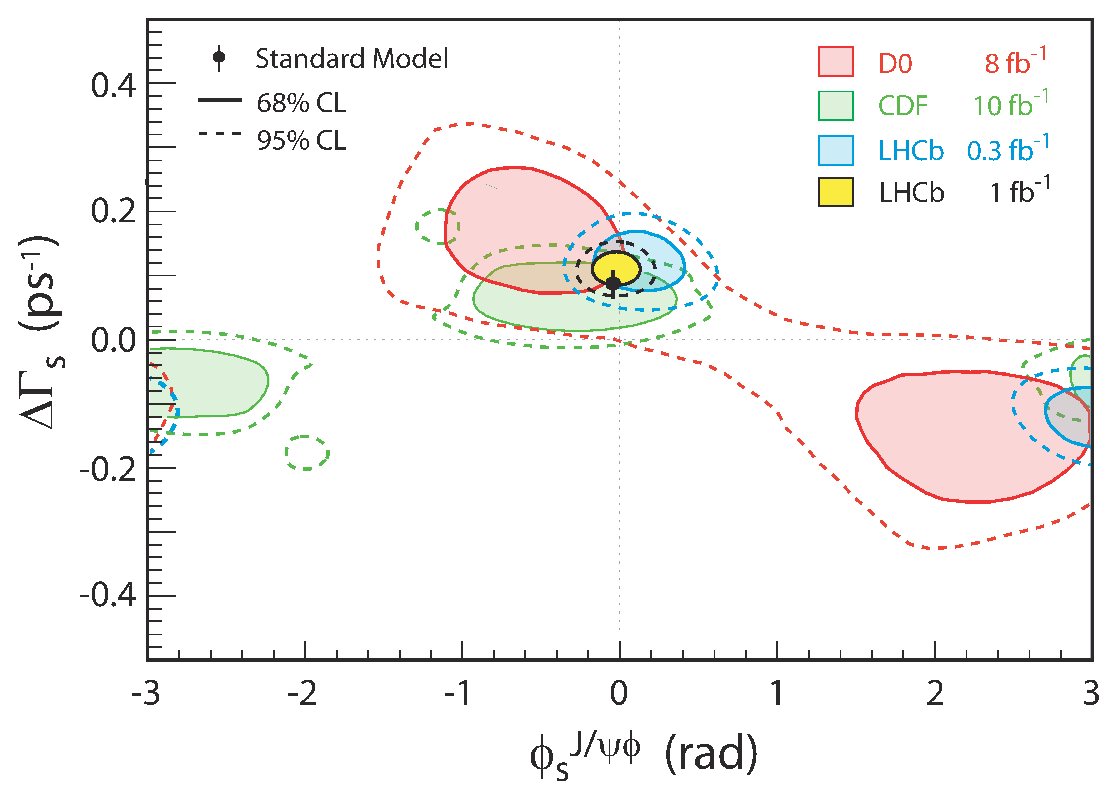
\includegraphics[scale=0.65,bb=50 300 580 700,clip=true]{Roger-plot}
    \vspace*{-1.0cm}
  \end{center}
  \caption{
    \small %captions should be a little bit smaller than main text
    Comparison of our result to those from other experiments.
    Note that the style of this figure differs slightly from that of Figure~\ref{fig:example}}
  \label{fig:roger}
\end{figure}

\clearpage


\addcontentsline{toc}{section}{References}
%\setboolean{inbibliography}{true}
\bibliographystyle{LHCb}
\bibliography{main,standard,LHCb-PAPER,LHCb-CONF,LHCb-DP,LHCb-TDR,local}
 
 
\end{document}
